\documentclass[pdftex,12pt,a4paper]{report}
\usepackage[utf8]{inputenc}
\usepackage[croatian]{babel}
\usepackage{amsmath}
\usepackage{graphicx}
\usepackage{pgf}

\usepackage{natbib}
\usepackage[colorlinks=true,linkcolor=black,unicode]{hyperref}

\usepackage{setspace} 

\usepackage[croatian]{algorithm2e}

\usepackage{tikz}
\usetikzlibrary{arrows}
\usetikzlibrary{shapes}
\usetikzlibrary{shadows}


\usepackage{subfig}
%\usepackage{caption}
\usepackage{float}
\usepackage{subfloat}
%\usepackage{mathptmx}
%\usepackage{courier}

\usepackage[scaled]{helvet}
\usepackage[colorlinks=true,linkcolor=black]{hyperref}
\usepackage{lscape}
\usepackage{titlesec}
\usepackage{fullpage}
\usepackage[parfill]{parskip}
\usepackage{mathtools}

\renewcommand{\labelitemi}{$\bullet$}
\renewcommand{\labelitemii}{$\circ$}
\renewcommand{\bibsection}{}

\titleformat{\chapter}[display]{\Huge\bfseries}{}{10pt}{\Huge\bfseries}
\titlespacing*{\chapter}{0pt}{-70pt}{10pt}


\newcommand{\HRule}{\rule{\linewidth}{0.5mm}}


\usepackage[top=2.5cm, bottom=2.5cm, left=3cm, right=2.5cm]{geometry}

\begin{document}

\begin{spacing}{1.5}

\begin{titlepage}

\begin{center}
	
	{\large SVEUČILIŠTE U ZAGREBU\\FAKULTET ELEKTROTEHNIKE I RAČUNARSTVA}
	
	\vfill

	\textbf{ \large Diplomski rad} \\


	\vspace{20pt}
	\textbf{\huge Ocjena učinkovitosti operatora križanja u genetskom programiranju}
	\vspace{40pt}
	
	\bigskip
	
	\begin{minipage}{1.0\textwidth}
	\begin{center} 
	Maja Kontrec
	\end{center}
	\end{minipage}
	\vfill

	% Bottom of the page
	{\large Zagreb, 2014.}
	
\end{center}

\end{titlepage}

\tableofcontents


\chapter{Uvod}
Genetsko programiranje predstavlja optimizacijsku tehniku iz skupine evolucijskih algoritama. Ono omogućava rješavanje teških optimizacijskih problema za koje, ili ne postoji egzaktna matematička metoda rješavanja, ili su nerješivi u nekom konačnom vremenu. 

Temeljeći se na imitaciji prirodnog evolucijskog procesa, ovaj algoritam djeluje uporabom genetskih operatora križanja, mutacije i selekcije. Genetski operatori u svakoj iteraciji modificiraju trenutnu populaciju potencijalnih rješenja - jedinki. Pri tome, operatori mutacije i križanja služe za pretraživanje samog prostora rješenja, dok selekcija služi kako bi bolje jedinke imale veću vjerojatnost preživljavanja nad onim lošijim. Ovime, genetsko programiranje obuhvaća veći dio prostora pretrage nego srodni algoritmi, koji unutar prostora svih mogućih rješenja pretražuju samo ona koja trenutno susjedna. Još jedna velika prednost genetskog programiranja nad drugim tehnikama optimizacije je ta da je ono neovisno o domeni, odnosno, može se koristiti za rješavanje širokog skupa različitih problema.

Unatoč navedenim prednostima genetskog programiranja, kao i genetskih algoritama općenito, danas još uvijek nije jednoznačan postupak odabira specifičnih podvrsta genetskih operatora, kao ni samog prikaza potencijalnih rješenja. Postupak postavljanja algoritma oslanja se na iskustvo samog postavljača te se temelji na eksperimentiranju. Eksperimentiranjem, potrebno je utvrditi koji su genetski operatori, zajedno s njihovim specifičnim parametrima, dobri za rješavanje problema.

U ovom radu, dan je pregled i opis postojećih genetskih operatora s naglaskom na operatore križanja. Ispitana je učinkovitost algoritma genetskog programiranja s obzirom na odabir operatora križanja za tri najčešće vrste problema koji se rješavaju genetskim programiranjem - simboličku regresiju, pronalazak logičkih funkcija i programe.


\chapter{Genetsko programiranje}
Genetsko programiranje podvrsta je genetskog algoritma. Najveća razlika između genetskog programiranja i genetskog algoritma je ta da je kod genetskog algoritma rješenje, odnosno jedinka, nepromjenjive duljine tijekom čitavog procesa evolucije.

U genetskom algoritmu, jedinka je predstavljena nizom informacija, primjerice nizom znamenki ili znakova, dok je kod genetskog programiranja jedinka predstavljena nekim slobodnijim oblikom, najčešće stablastom strukturom. Stablasta struktura pritom može predstavljati izvršivi program ili pak neki logički ili matematički izraz. Osim najčešće stablaste strukture, jedinka genetskog programiranja također može biti predstavljena i linearno, nizom informacija promjenjive duljine (primjerice, u slučaju da jedinka predstavlja program, može biti predstavljena nizom izvršivih instrukcija).

\section{Tijek algoritma}

Sam algoritam genetskog programiranja oponaša prirodnu evoluciju. Nakon stvaranja, skup jedinki koji čini populaciju algoritma, prolazi kroz proces evolucije pronalazeći rješenje danog problema. Tijek algoritma prikazan je na slici \ref{tijek}.

Algoritam započinje inicijalizacijom početne populacije rješenja, odnosno jedinki. Nakon stvaranje početne populacije, potrebno je evaluirati svaku zasebnu jedinku. Evaluacija se pritom odnosi na izračun dobrote (\textit{eng. fitness}) jedinke; svojstva koje govori o tome koliko je ona kvalitetno rješenje. Pomoću dobrote, jedinke su međusobno usporedive.

Inicijalizacijom populacije započinje prva generacija algoritma. Na početku svake generacije provjerava se da li je zadovoljen kriterij zaustavljanja algoritma. Ukoliko je, algoritam završava sa svojim izvođenjem, a u suprotnom, sljedeći korak algoritma je selekcija jedinki. 
Selekcijom se odabiru jedinke koje će preživjeti i sudjelovati u križanju u ulozi roditelja, te jedinka koja će biti zamijenjena njihovim potomkom.

Nakon dobivanja nove jedinke križanjem, ona se mutira s određenom vjerojatnosti mutacije te se izračunava njena nova dobrota.

Ova tri operatora; selekcija, mutacija i križanje, predstavljaju imitaciju evolucije u samom algoritmu. Isto kao u prirodi, u sljedeću generaciju ulaze samo najjače jedinke čiji se genetski materijal kombinira u nešto novo, pokušavajući naći kombinaciju materijala koja će donijeti poboljšanje.


\begin{figure}[H]
	\centering
	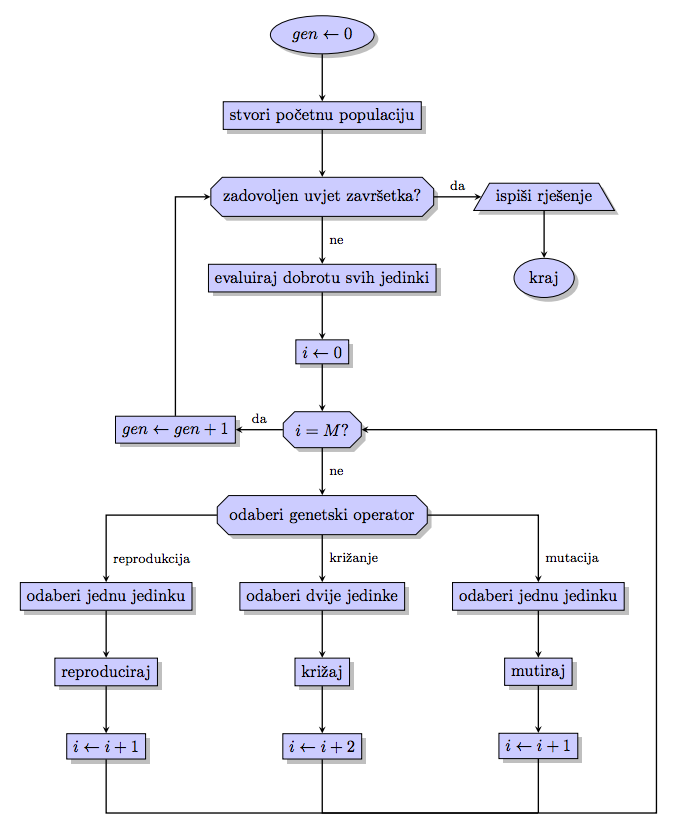
\includegraphics[scale=0.6]{./slike/blokDijagram.png}
	\caption{Tijek izvršavanja algoritma genetskog programiranja (slika preuzeta iz \cite{kokan})}
	\label{tijek}
\end{figure}

\section{Stablasta jedinka}
Najčešći oblik jedinke korišten u genetskom programiranju je stablo. Razlog zašto je tome tako je činjenica da se stablo može interpretirati na više različitih način. Stablo je pogodno za prikaz programskih jedinki, kao i prikaz jedinki koji predstavljaju neki matematički ili logički izraz.


\subsection{Stablo kao program}
Pomoću stabla lako je modelirati neki izvršivi program. Jedan od poznatijih problema rješavanih genetskim programiranjem je problem umjetnog mrava (\textit{eng. Artificial ant problem} \cite{koza}). U ovom slučaju, jedinka predstavlja ponašanje mrava unutar neke okoline. Cilj algoritma je evoluirati ponašanje koje će efikasno pronalaziti hranu unutar te okoline.

 Nezavršni znakovi unutar stabla pritom donose odluke o ponašanju, dok završni znakovi predstavljaju samo ponašanje pojedinog mrava. Na slici \ref{ant} prikazana je jedna takva jedinka. 

\begin{figure}
	\centering

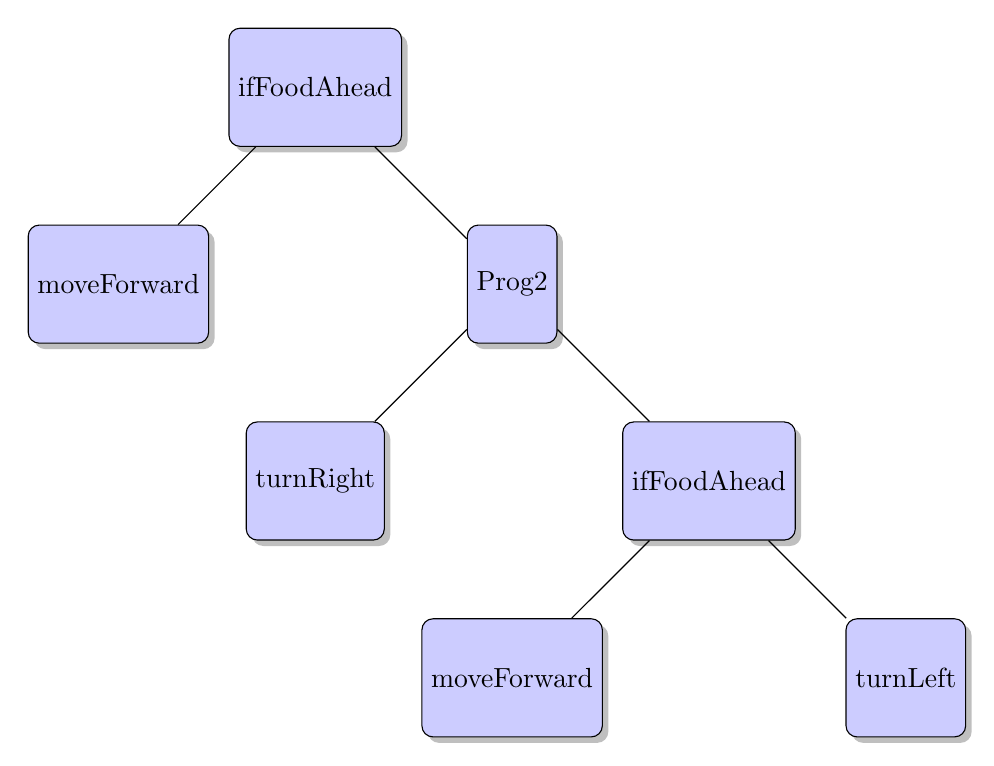
\begin{tikzpicture}
[sibling distance=50mm, level distance=25mm,
every node/.style={fill=blue!20,rectangle, rounded corners,draw,drop shadow, minimum height=1.5cm}]


  \node {ifFoodAhead}
      child {node {moveForward}}
      child {node {Prog2}
        child {node {turnRight}}
        child {node {ifFoodAhead}
        	child{node {moveForward}}
        	child{node {turnLeft}}
        }
      };
\end{tikzpicture}

	\caption{Primjer jedinke programa umjetnog mrava}
	\label{ant}
\end{figure}


Nezavršni znakovi koji grade jednu ovakvu jedinku su:

\begin{enumerate}

  \item \textbf{If food ahead} - provjerava da li se nalazi hrana ispred mrava - ako da izvršava lijevu granu, ako ne, izvršava desnu granu.
  \item \textbf{Prog2} - slijedno izvršava lijevu, te zatim desnu granu.
  \item \textbf{Prog3} - slijedno izvršava (s lijeva na desno) svaku od 3 pridružene grane.

\end{enumerate}

Završni znakovi koji grade ovu jedinku su:
\begin{enumerate}

  \item \textbf{move forward} - pomiče mrava za jedno mjesto unaprijed.
  \item \textbf{turn right} - okreće mrava u desno.
  \item \textbf{turn left} - okreće mrava u lijevo.

\end{enumerate}

Ovakva stabla vrlo je jednostavno za interpretirati - kreće se od vršnog čvora, te se prema pravilima čvorova prolazi kroz stablo i izvršavaju dane instrukcije. Pseudokod koji opisuje stablo prikazano na slici \ref{ant} dan je ispod (\ref{pseudokod}).

\begin{algorithm}
\eIf {food ahead} {
	move forward;
} {
	turn right;\\
	\eIf {food ahead} {
		move forward;
	} {
		turn left;
	}
}

	\caption{Pseudokod jedinke prikazane na slici \ref{ant}}
	\label{pseudokod}
	\centering
\end{algorithm}

\subsection{Stablo kao logički izraz}

Osim programa, stablo može reprezentirati i neki logički izraz. Pri tome, nezavršni čvorovi predstavljaju logičke funkcije, dok završni čvorovi predstavljaju varijable. Logička funkcija predstavljena takvim stablom jednostavno se može izlučiti \textit{in-order} obilaskom stabla. Jedna ovakva jedinka dana je na slici \ref{logTree}. 
\\
\begin{figure}[H]
	\centering
	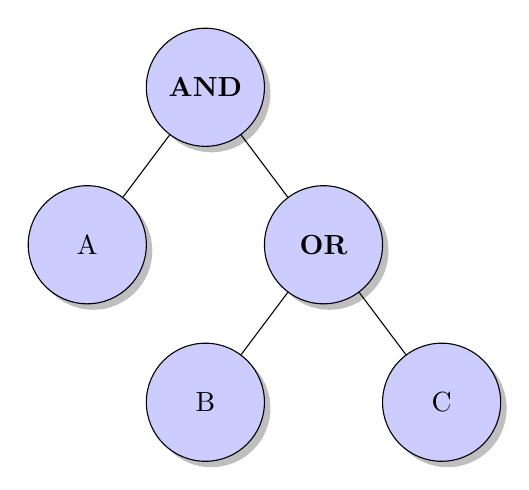
\begin{tikzpicture}
	[sibling distance=30mm, level distance=20mm,
	every node/.style={fill=blue!20,circle,draw,drop shadow, minimum height=1.5cm}]
	\node {\textbf{AND}}
    		child {node {A}}
    		child {node {\textbf{OR}}
        		child {node {B}}
        		child {node {C}}
      		};
	\end{tikzpicture}
	\caption{Stablo koje predstavlja logički izraz $A  \cdot (B + C)$}
	\label{logTree}
\end{figure}


\subsection{Stablo kao matematički izraz}

Jednako kao i logičke izraze, stablo može predstavljati neki matematički izraz. Kao i u prethodnom slučaju, matematički izraz se iz stabla može izlučiti \textit{in-order} obilaskom. Na slici \ref{matTree} prikazana je jedna takva jedinka.

\begin{figure}[H]
	\centering
	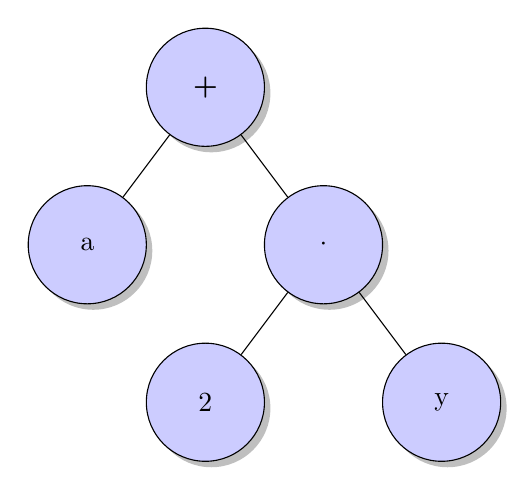
\begin{tikzpicture}
	[sibling distance=30mm, level distance=20mm,
	every node/.style={fill=blue!20,circle,draw,drop shadow, minimum height=1.5cm}]
	\node {\textbf{+}}
    		child {node {a}}
    		child {node {\textbf{$\cdot$}}
        		child {node {2}}
        		child {node {y}}
      		};
	\end{tikzpicture}
	\caption{Stablo koje predstavlja matematički izraz $a + 2 \cdot y$}
	\label{matTree}
\end{figure}

\section{Dobrota jedinke}

Dobrota (\textit{eng. fitness}) jedinke predstavlja njenu kvalitetu - označava koliko dobro ta jedinka rješava dani problem. Dobrota je najčešće predstavljena realnim brojem, te omogućuje mođusobnu usporedivost jedinki. Na osnovi iznosa dobrote pojedine jedinke provodi se selekcija unutar populacije.

Definiranje funkcije dobrote kojom se dobiva sam iznos dobrote jedan je od problema koji se pojavljuje prilikom postavljanja samog algoritma. Funkcija dobrote razlikuje se za svaki pojedini problem.

 Lako je uočljivo kako dobrota uvelike definira smjer napretka algoritma, te je stoga pitanje pronalaska adekvatne funkcije dobrote vrlo važno za kvalitetu samog algoritma. 

\section{Operatori selekcije}
Selekcija u genetskom programiranju osigurava prijenos kvalitetnog genetskog materijala u buduće generacije birajući jedinke koje će sudjelovati u reprodukciji  \cite{nenr}. Operatori selekcije se prema metodi odabira jedinki dijele na:

\begin{itemize}
\item proporcionalne selekcije - odabiru jedinke s vjerojatnošću koja je proporcionalna njihovoj dobroti
\item rangirajuće selekcije - odabiru jedinke s vjerojatnošću koja ovisi o rangu  dobrote jedinke (u usporedbi s dobrotama ostalih jedinki)
\end{itemize}

Ovisno o načinu prenošenja genetskog materijala boljih jedinki u iduću iteraciju načini selekcije se dijele na:

\begin{itemize}
	\item generacijske selekcije - selekcija direktno bira bolje jedinke koje sudjeluju u križanju
	\item eliminacijske selekcije - selekcija bira lošije jedinke za eliminaciju; bolje jedinke 				u ovom slučaju preživljavaju selekciju
\end{itemize}

\subsection{Generacijska selekcija}

Generacijska selekcija direktno odabire dvije jedinke koje će sudjelovati u reprodukciji, kopirajući one bolje jedinke u novu populaciju - nazvanu međupopulacijom. Broj jedinki u međupopulaciji manji je nego onaj u originalnog populaciji. Budući da sve jedinke populacije neće preživjeti selekciju, u međupopulaciju se najčešće stavljaju duplikati preživjelih jedinki. Iz ovoga se vidi očiti problem koji nastaje ovakvom selekcijom - smanjuje se raznovrsnost genetskog materijala koji će sudjelovati u reprodukciji. Posljedično, nedostatak genetske raznovrsnosti doprinosi usporavanju procesa evolucije.

Iz opisanog je vidljivo kako generacijska selekcija stvara čvrstu granicu između generacija - svaka jedinka postoji točno jednu generaciju.


\subsection{Eliminacijska selekcija}

Za razliku od generacijske selekcije, kod koje postoji čvrsta granica između generacija, u eliminacijskoj selekciji dobre jedinke preživljavaju više generacija. Eliminacijska selekcija nadomješta \textit{M} jedinki novim jedinkama koje su nastale reprodukcijom onih boljih. Pri tome, parametar \textit{M} se naziva mortalitetom.

Eliminacijska selekcija svojim djelovanjem ne stvara duplikate jedinki čime se otklanja osnovni problem generacijske selekcije.

\section{Operatori križanja}

Operatori križanja obavljaju rekombinaciju genetskog materijala, stvarajući jednu novu jedinku koja nastaje kombinacijom neke druge dvije, roditeljske jedinke. U slučaju genetskog programiranja gdje je jedinka predstavljena u obliku stabla, križanje se svodi na spajanje dvaju podstabla roditelja u novo stablo djeteta (slika \ref{crx}). Zasebni operatori križanja detaljno će biti opisani u idućem poglavlju.

\begin{figure}[H]
 	\centering


	\begin{tikzpicture}
	[sibling distance=25mm, level distance=15mm,
	every node/.style={fill=blue!20,circle,draw,drop shadow, minimum height=1cm}]
	\node {\textbf{+}}
    		child {node {a}}
    		child {node {\textbf{$\cdot$}}
        		child {node {2}}
        		child {node {y}}
      		};
	};

\begin{scope}[xshift=7cm]
	\node {\textbf{+}}
    		child {node {a}
        		child {node {2}}
        		child {node {y}}
      		}
    		child {node {\textbf{$sin$}}
			child {node {x}}};
	};
\end{scope}

\begin{scope}[xshift=11.5cm]

	\node  {\textbf{+}}
    		child {node {a}}
    		child {node {\textbf{$sin$}}
        		child {node {x}}
      		};
	};

\end{scope}
	\end{tikzpicture}


	\caption{Primjer jednostavnog križanja stabala}
	\label{crx}
\end{figure}


\section{Operatori mutacije}

Mutacija je operator koji djeluje direktno na pojedinu jedinku. Kao i u prirodi, mijenja jedan dio jedinke. Jedinka mutira s određenom vjerojatnošću, koji je uobičajeno broj reda veličine 0.1. Na slici \ref{mutSimple} prikazana je jednostavna mutacija koja nasumično mijenja jedan čvor stabla. 

Uobičajene metode mutacije uključuju:

\begin{itemize}
	\item zamjena nasumično odabranog podstabla novim, također nasumično generiranim stablom
	\item zamjena nasumično odabranog čvora njegovim komplementom
	\item zamjena slučajno odabranog čvora čvorom istog tipa
	\item zamjena slučajno odabranog podstabla završnim čvorom
\end{itemize}
\begin{figure}[H]
 	\centering


\begin{tikzpicture}
	[sibling distance=25mm, level distance=15mm,
	every node/.style={fill=blue!20,circle,draw,drop shadow, minimum height=1cm}]

\begin{scope}[xshift=0cm]
	\node   {\textbf{+}}
    		child {node {$cos$}
    			child {node {-}
    				child {node {x}}
    				child {node {y}}
    			}
    		}
    		child {node {\textbf{$/$}}
			child {node  {x}}
			child {node  {y}}	
		};
	};
\end{scope}

\begin{scope}[xshift=7cm]
	\node   {\textbf{+}}
    		child {node [fill=red!20] {$sin$}
    			child {node {-}
    				child {node {x}}
    				child {node {y}}
    			}
    		}
    		child {node {\textbf{$/$}}
			child {node  {x}}
			child {node  {y}}	
		};
	};
\end{scope}

\end{tikzpicture}


	\caption{Primjer jednostavne mutacije. Desno: jedinka prije mutacije, lijevo: jedinka nakon mutacije}
	\label{mutSimple}
\end{figure}

Mutacija je vrlo korisna u slučaju kada jedinka zapne u nekom od lokalnih minimuma. Naime, mutacija može značajno promijeniti jedinku, te ju tako dosta udaljiti od trenutnog prostora pretraživanja. 


\chapter{Operatori križanja}
Utjecaj operatora križanja već je neko vrijeme jedna od zanimljivijih tema genetskog programiranja. Često se postavlja pitanje je li uopće algoritam učinkovitiji kada se koriste operatori križanja ili je jednostavnije i bolje jednostavno odbaciti takav način i okrenuti se nekim drugim pristupima koji posjeduju veću razinu determinizma.

Na ovu temu, provedeno je nekoliko istraživanja. John R. Koza u \cite{koza} je uključio jednostavnu usporedbu algoritama genetskog programiranja sa i bez operatora križanja (koristeći mutaciju u oba slučaja), te pokazao da postojanje operatora križanja uvelike doprinosi kvaliteti konačnog rješenja. Međutim, istraživanje nije detaljno opisao niti je spomenuo da je koristio neke statističke metodi pri tome. Luke i Spector \cite{luke} objavili su usporedbu operatora križanja i mutacije na četiri različita problema. Nisu našli nikakve važnije razlike između isključivog korištenja mutacije ili križanja. White i Poulding \cite{rigo} zaključili su da operator križanja nema preveliku prednost pred operatorom mutacije. 

U sljedećim poglavljima, detaljno će biti opisani različiti operatori križanja u genetskom programiranju, te će biti opisana do sada provedena istraživanja sa spomenutim operatorima. Ova istraživanja, osim predstavljanja pojedinog operatora, uključuju i njegovu usporedbu s ostalim operatorima križanja. U kasnijim poglavljima biti će predstavljena istraživanja, zajedno s njihovim zaključcima, provedena u sklopu izrade ovoga rada.

\section{Jednostavno križanje}
Jednostavno križanje (\textit{eng. subtree crossover}) predstavljeno je u \cite{crxSimple}. Ovo križanje ujedno je i najjednostavnije i najkorištenije križanje u genetskom programiranju.

Nova jedinka nastaje spajanjem dvaju nasumično odabranih podstabala roditelja. U svakom roditelju odabire se po jedna točka prekida koja označava mjesta na kojima će se dogoditi križanje.

Često, odabir točaka prekida ne odvija se uniformno. Naime, tipični čvorovi stabala imaju prosječni faktor grananja \footnote{broj djece pojedinog čvora} (\textit{eng. branching factor}) jednak barem 2, što uzrokuje da je većina čvorova nekog stabla u stvari list, odnosno, završni znak. Posljedično, ukoliko bi ovo križanje biralo točke prekida na uniforman način, došlo bi do vrlo male količine razmijenjenog genetskog materijala: nerijetko bi se dogodilo da križanjem nastane nova jedinka koja je gotovo identična jednom od roditelja - od tog roditelja, razlikovala bi se u samo jednom listu koji pripada onom drugom roditelju. Kako bi se razriješio ovaj problem, Koza \cite{koza} je predložio kasnije često korišten pristup - prilikom odabira točke prekida, postavlja se vjerojatnost odabira nezavršnog čvora na 0.9, a vjerojatnost odabira lista stabla kao točke prekida na 0.1.

Ovakvim križanjem, dobivaju se dvije različite, nove jedinke. Iako neke implementacije ovog operatora uzimaju oba dva djeteta u novu generaciju, češće je slučaj da se uzima samo jedno dijete. Na slici \ref{crxSimple} prikazan je primjer jednostavnog križanja.

\begin{figure}[H]
 	\centering


\begin{tikzpicture}
	[sibling distance=25mm, level distance=15mm,
	every node/.style={fill=blue!20,circle,draw,drop shadow, minimum height=1cm}]
	
	
	\node  {\textbf{+}}
    		child {node {a}}
    		child {node [fill=green!20]  {\textbf{$sin$}}
        		child {node  {x}}
      		};
	};

\begin{scope}[xshift=7cm, yshift=0cm]
	\node {\textbf{+}}
    		child {node {$cos$}
        		child {node {y}}
      		}
     		child {node [fill=yellow!20]  {\textbf{$\cdot$}}
        		child {node {2}}
        		child {node {y}}
      		};
	};
\end{scope}

\begin{scope}[xshift=0cm, yshift=5cm]

	\node {\textbf{+}}
    		child {node {a}}
    		child {node [fill=yellow!20]  {\textbf{$\cdot$}}
        		child {node {2}}
        		child {node {y}}
      		};
	};
\end{scope}

\begin{scope}[xshift=7cm, yshift=5cm]
	\node {\textbf{+}}
    		child {node {$cos$}
        		child {node {y}}
      		}
    		child {node [fill=green!20] {\textbf{$sin$}}
			child {node {x}}};
	};
\end{scope}

\end{tikzpicture}


	\caption{Primjer jednostavnog križanja stabala}
	\label{crxSimple}
\end{figure}

Na prvom roditelju (gornji lijevi kut) odabrana točka prekida označena je žutom bojom, a na drugom roditelju zelenom bojom. Na donjem dijelu slike vidljivi su rezultati križanja - dva moguća potomka nastala križanjem ova dva roditelja. Lijevo dijete nastalo je spajanjem podstabla prvom roditelja koje se nalazilo iznad točke prekida i podstabla drugog roditelja koje se nalazilo ispod njegove točke prekida. Desno dijete nastalo je suprotnom kombinacijom - spojeno je podstablo ispod točke prekida prvog roditelja i podstablo iznad točke prekida drugog roditelja.

Budući da je ovaj operator križanja najstariji operator, u daljnjem tekstu uglavnom će služiti kao osnovna usporedba učinkovitosti. Za očekivati je da će svaki drugi operator predstavljen u idućim poglavljima donijeti poboljšanja u odnosu na ovaj operator.

\section{Križanje s jednom točkom prekida}
Tijekom biološke reprodukcije, genetski materijal roditelja rekombinira se na takav način da se određeni geni prenose na otprilike jednako mjesto unutar kromosoma kao što su bili smješteni unutar onog roditeljskog. Ovo se konceptualno razlikuje od načina jednostavnog križanja, gdje je moguće pomicanje podstabala na potpuno drugačiju poziciju od one izvorišne.

Operatori križanja koji čuvaju poziciju genetskog materijala nazivaju se homolognima. Ovaj operator predstavlja jednu inačicu homolognog križanja i razlikuje se od kasnije spomenutog homolognog operatora križanja. Ovakvi operatori češće su korišteni u linearnom genetskom programiranju gdje je pojam homologije puno intuitivniji i uočljiviji, za razliku od stabala gdje se homolognost može interpretirati na više različitih načina. Posljedično višestrukoj interpretaciji homologije unutar stabala postoji i više vrsta homolognih operatora križanja. 

\begin{figure}[H]
 	\centering


\begin{tikzpicture}
	[sibling distance=25mm, level distance=15mm,
	every node/.style={fill=blue!20,circle,draw,drop shadow, minimum height=1cm}]

\begin{scope}[xshift=0cm]

	\node  [fill=yellow!20]  {\textbf{+}}
    		child {node [fill=yellow!20]  {$cos$}
    			child {node  [fill=yellow!20] {-}
    				child {node{x}}
    				child {node{y}}
    			}
    		}
    		child {node [fill=yellow!20]  {\textbf{$\cdot$}}
        		child {node [fill=yellow!20]  {2}}
        		child {node [fill=yellow!20]  {y}}
      		};
	};
\end{scope}

\begin{scope}[xshift=7cm]
	\node  [fill=yellow!20]  {\textbf{+}}
    		child {node  [fill=yellow!20] {$sin$}
        		child {node  [fill=yellow!20] {y}}
      		}
    		child {node [fill=yellow!20] {\textbf{$/$}}
			child {node [fill=yellow!20]  {x}}
			child {node [fill=yellow!20]  {y}}	
		};
	};
\end{scope}

\end{tikzpicture}


	\caption{Zajedničko područje dva roditelja}
	\label{crxOnePointCommon}
\end{figure}

Križanje s jednom točkom prekida predstavljeno je u \cite{crxOnePoint}, te je prvo križanje koje uzima u obzir homologiju gena. Temelji se na odabiru zajedničke točke križanja unutar roditelja. Pri tome, zajednička točka križanja može se odabrati samo unutar zajedničkih područja roditelja - područja u kojima podstabla oba roditelja imaju potpuno jednak oblik. Primjer zajedničkih područja dan je na slici \ref{crxOnePointCommon}, gdje je zajedničko područje dva roditelja označen žutom bojom. Zajednička područja odgovaraju homologiji u smislu da je velika vjerojatnost da podstabla jednakih oblika obavljaju jednaku ili sličnu funkciju. Također, budući da su podstabla jednakog oblika, pozicija određenog gena je intuitivna i jednoznačna.

Na slici \ref{crxOnePoint} prikazan je rezultat križanja roditelja sa slike \ref{crxOnePointCommon}, gdje je za točku prekida odabran čvor $cos$ unutar prvog, odnosno $sin$ unutar drugog roditelja. 

\begin{figure}[H]
 	\centering


\begin{tikzpicture}
	[sibling distance=25mm, level distance=15mm,
	every node/.style={fill=blue!20,circle,draw,drop shadow, minimum height=1cm}]

\begin{scope}[xshift=0cm]

	\node {\textbf{+}}
    		child {node [fill=red!20]  {$sin$}
    				child {node [fill=red!20]{y}}
    		}
    		child {node {\textbf{$\cdot$}}
        		child {node{2}}
        		child {node {y}}
      		};
	};
\end{scope}

\begin{scope}[xshift=7cm]
	\node   {\textbf{+}}
    		child {node [fill=red!20] {$cos$}
    			child {node [fill=red!20]{-}
    				child {node [fill=red!20]{x}}
    				child {node [fill=red!20]{y}}
    			}
    		}
    		child {node {\textbf{$/$}}
			child {node  {x}}
			child {node  {y}}	
		};
	};
\end{scope}

\end{tikzpicture}


	\caption{Rezultat križanja roditelja sa slike \ref{crxOnePointCommon}}
	\label{crxOnePoint}
\end{figure}

\subsection{Dosadašnji rezultati}

U \cite{onePointExp} provedeno je istraživanje o učinkovitosti ovog operatora nad $n$-paritetnim problemom \footnote{rješenje ovog problema je pronaći funkciju $n$ varijabli koja je za parni broj istinitih varijabli istinita}, za $n$ = 3, 4. Na slici \ref{even3par} prikazani su rezultati za rješavanje 3-paritetnog problema. Ovdje, stupac \textit{Depth } označava dubinu dobivenog rješenja, \textit{$p_m$}  vjerojatnost mutacije, te je u ostalim stupcima prikazan napor uložen u izgradnju točnog rješenja s veličinom jedinke u zagradi. Analogno ovome u \ref{even4par} prikazan je jednak scenarij za 4-paritetni problem.

Na slikama je vidljivo kako ovo križanje u prosjeku daje dosta manja rješenja od jednostavnog križanja, no da je do takvih rješenja nešto teže doći. Ovime se može reći kako ovo križanje ima prednost nad jednostavnim križanjem - brzina pronalaska konačnog rješenja u genetskom programiranju ionako nije jedan od bitnih faktora koji ukazuje na uspješnost samog algoritma.

 \begin{figure}[H]
	\centering
	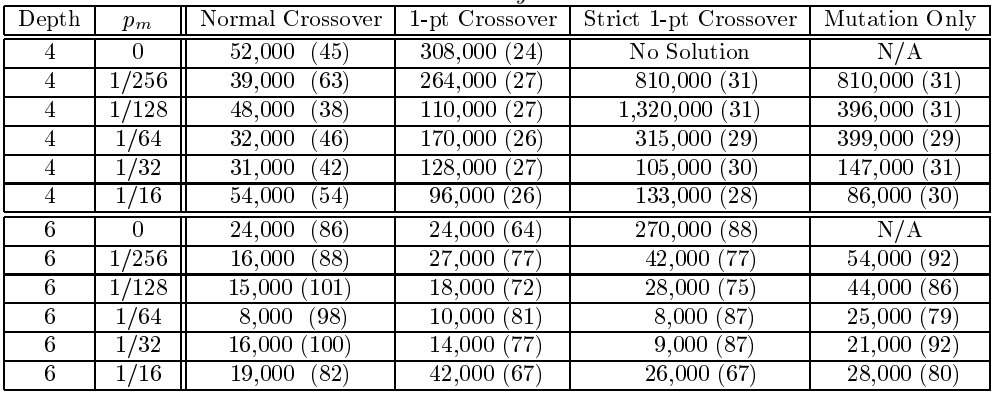
\includegraphics[scale=0.4]{./slike/even3par.png}
	\caption{Rezultati rješavanja 3-paritetnog problema}
	\label{even3par}
\end{figure}

 \begin{figure}[H]
	\centering
	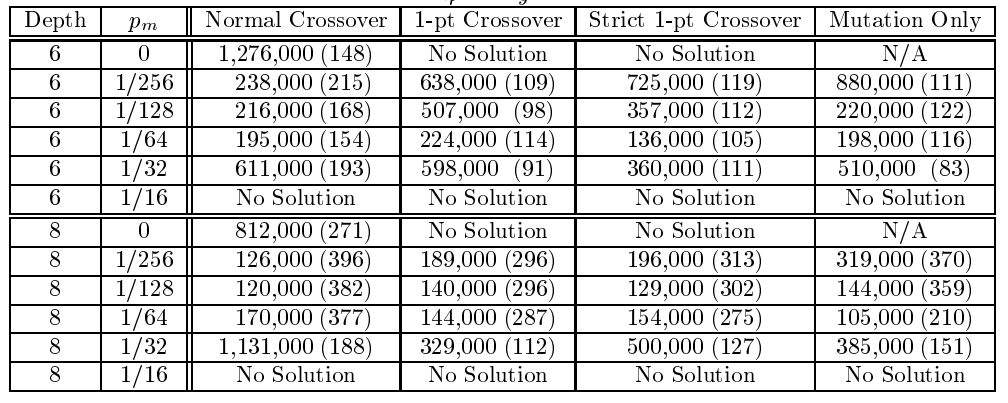
\includegraphics[scale=0.4]{./slike/even4par.png}
	\caption{Rezultati rješavanja 4-paritetnog problema}
	\label{even4par}
\end{figure}


\section{Križanje s očuvanjem konteksta}
Križanje s očuvanjem konteksta \cite{crxContext} također križa dvije jedinke na mjestu točke prekida. Ovaj operator u stablo uvodi koordinate svakog pojedinog čvora. Koordinate označavaju put unutar stabla kojim se dolazi do određenog čvora. Primjer koordinata čvorova stabla dan je na slici \ref{crxContextCoordinates}. Ovakve koordinate jednostavno i jednoznačno opisuju poziciju određenog čvora unutar stabla. Primjerice, čvor s koordinatama (1,1,2) nalazi se u drugoj grani podstabla koje se nalazi u prvoj grani prvog podstabla.

\begin{figure}[H]
 	\centering
\begin{tikzpicture}
	[sibling distance=45mm, level distance=25mm,
	every node/.style={fill=blue!20,circle,draw,drop shadow, minimum height=1.5cm}]
	\node   {-}
    		child {node  {1}
    			child {node {1,1}
    				child {node{1,1,1}}
    				child {node{1,1,2}}
    			}
    		}
    		child {node {2}
        		child {node  {2,1}}
        		child {node {2,2}}
      		};
	};

\end{tikzpicture}


	\caption{Koordinate čvorova stabla}
	\label{crxContextCoordinates}
\end{figure}

\subsection{Križanje s jakim očuvanjem konteksta}
Križanje s jakim očuvanjem konteksta (\textit{eng. strong context preserved crossover - SCPC}) dopušta križanje samo onih podstabala koja imaju potpuno jednake koordinate korijena. Ovakav operator postavlja vrlo stroga ograničenja na proces križanja. U \cite{crxContext} pokazano je kako koristeći ovakav operator, postoji velika vjerojatnost da podstablo generirano na određenoj razini na određenom mjestu stabla nikada ne uspije prijeći u potomke. Ovo bi kroz generacije prouzročilo smanjivanje genetske raznolikosti, što je u potpunoj suprotnosti ulozi operatora križanja. Kako bi se ublažio ovakav utjecaj operatora križanja s jakim očuvanjem konteksta, on se nikada ne koristi ekskluzivno, već u kombinaciji s nekim drugim operatorima križanja.

\subsection{Križanje sa slabim očuvanjem konteksta}
Kako bi se ublažila rigoroznost križanja s jakim očuvanjem konteksta, D'haeseleer \cite{crxContext} je također predložio blažu inačicu ovog križanja - križanje sa slabim očuvanjem konteksta (\textit{eng. weak context preserved crossover - WCPC}). Ova inačica kontekstnog križanja predstavlja pojednostavljenje križanja s jakim očuvanjem konteksta. Korijen podstabla prvog roditelja koje će sudjelovati u križanju odabire se između skupa čvorova za koje postoji odgovarajući čvor u drugom roditelju (jednako kao i kod križanja s jakim očuvanjem konteksta). Podstablo u drugom roditelju koje će sudjelovati u križanju odabire se tako da mu vršni čvor odgovara vršnom čvoru odabranog podstabla prvog roditelja. Drugim riječima, ako su $T1$ i $T2$ važeći odabiri podstabala za križanje s jakim očuvanjem konteksta, tada su $T1$ i $T2' \subseteq T2$ važeći odabiri podstabala za križanje sa slabim očuvanjem konteksta.

\subsection{Dosadašnji rezultati}
U \cite{crxContext} obavljena su četiri različita eksperimenta koja pokazuju učinkovitost ovih operatora križanja. U nastavku su opisani ti eksperimenti.

\subsubsection{Robot sa sposobnosti izmicanja preprekama}
Cilj ovog problema je evoluirati robota koji pi prešao što veću površinu zadanog prostora, zaobilazeći pritom prepreke koje mu se nađu na putu. Pri tome, broj pokreta robota je ograničen na neki fiksni broj $n$. 

Rezultati ovog eksperimenta pokazali su kako ovo križanje nije dobro za evoluciju rješenja danog problema. Budući da evoluirani robot samo jednom izvršava svoj program predstavljen stablom, to stablo bi trebalo biti veliko i opisivati svaki korak robota. Budući da ova križanja, a pogotovo križanje s jakim očuvanjem konteksta ne potiče prijenos krajnjih podstabala rješenja, dobiven rezultat bio je i za očekivati. Na slici \ref{robot} dana je usporedba učinkovitosti uobičajenog (jednostavnog) operatora križanja, kombinacije jednostavnog i križanja s jakim očuvanjem konteksta (u omjeru 1:1) i križanja s jakim očuvanjem konteksta. Vidljivo je kako je jednostavno križanje superiorno nad kontekstnim križanjima za rješavanje ovog problema.

\begin{figure}[H]
	\centering
	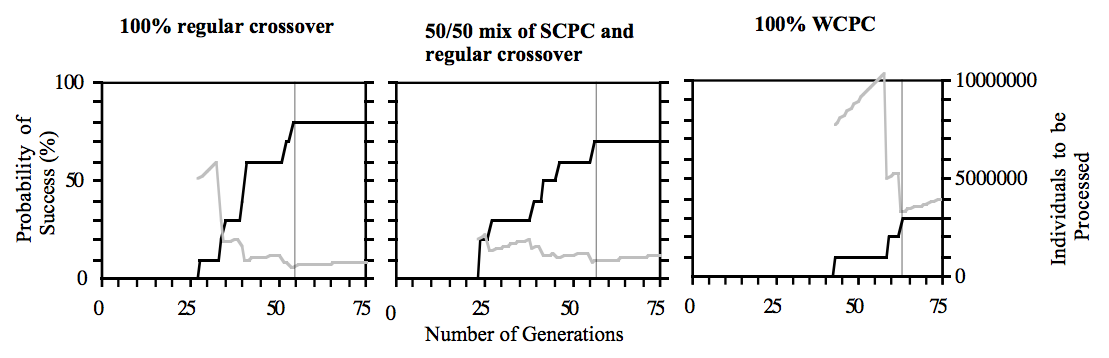
\includegraphics[scale=0.4]{./slike/robot.png}
	\caption{Učinkovitost različitih operatora križanja za problem robota sa sposobnošću izmicanja prepreka. lijevo: jednostavno križanje, sredina: kombinacija jednostavnog i križanja sa slabim očuvanjem konteksta, desno:  križanje s jakim očuvanjem konteksta}
	\label{robot}
\end{figure}


\subsubsection{Iterirana inačica robota sa sposobnosti izmicanja preprekama}
Za razliku od prethodno opisanog problema, gdje se program predstavljen stablom izvršava samo jedan put, u ovom problemu unutar dopuštenog broja koraka dopušteno je izvoditi program po nekoliko puta. Ovakvo ponašanje u stvari je i prirodnije od jednostrukog izvršavanja stabla, i očekivano je da će u ovom slučaju kontekstni operatori djelovati efikasnije nego kod rješavanja prethodnog problema. Na slici \ref{robotIt} prikazana je usporedba učinkovitosti operatora križanja za ovaj problem. Vidljivo je kako je kombinacija jednostavnog i križanja s jakim očuvanjem konteksta (u omjeru 1:3) djelovala najbolje pri rješavanju ovog problema.

\begin{figure}[H]
	\centering
	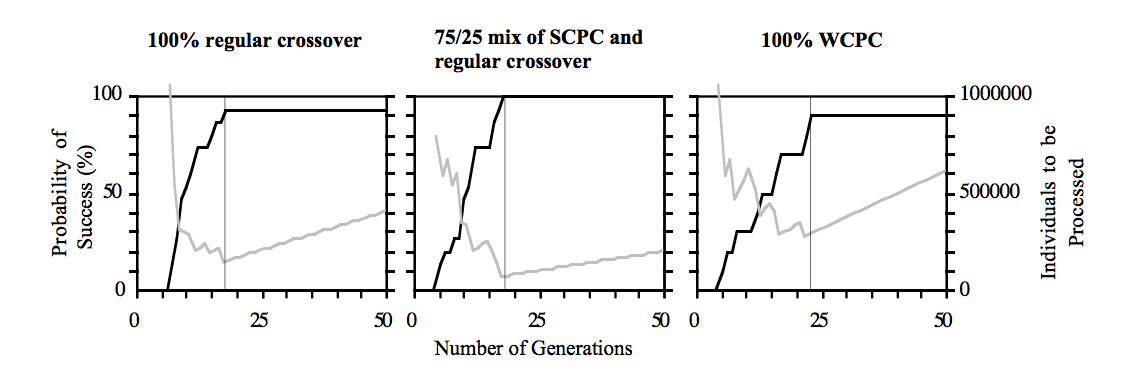
\includegraphics[scale=0.4]{./slike/robotIt.png}
	\caption{Učinkovitost različitih operatora križanja za iterativni problem robota sa sposobnošću izmicanja prepreka. lijevo: jednostavno križanje, sredina: kombinacija jednostavnog i križanja sa slabim očuvanjem konteksta, desno:  križanje s jakim očuvanjem konteksta}
	\label{robotIt}
\end{figure}



\subsubsection{11 - multipleksor}
Cilj boolean 11 - multipleksor problema je pronaći logičku funkciju koja za 3 predana adresna bita daje podatak veličine 8 bita. U ovom problemu, kombinacija jednostavnog i križanja s jakim očuvanjem konteksta (u omjeru 1:1) pokazala se daleko boljim odabirom za operator križanja nego jednostavno križanje. Križanje sa slabim očuvanjem konteksta se i u ovom eksperimentu pokazalo prilično inferiorno ostalim dvama operatorima. Na slici \ref{mux} prikazana je usporedba učinkovitosti različitih operatora križanja na ovaj problem.

\begin{figure}[H]
	\centering
	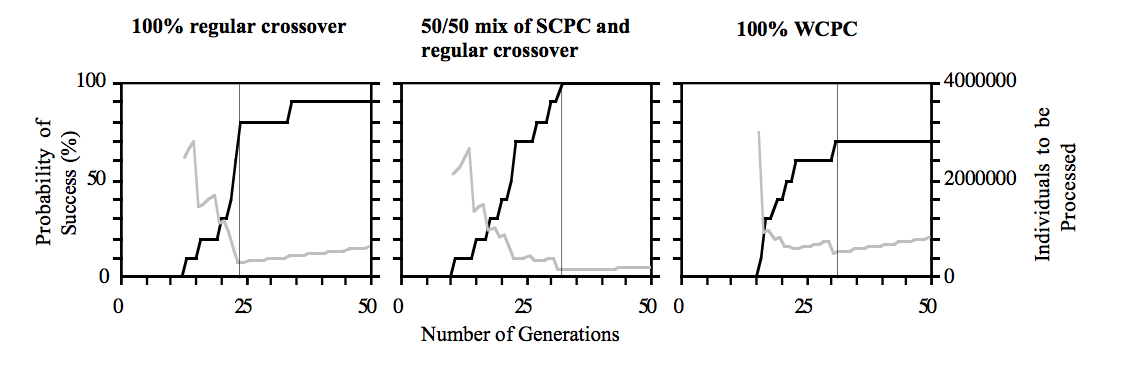
\includegraphics[scale=0.4]{./slike/mux.png}
	\caption{Učinkovitost različitih operatora križanja za problem boolean 11 - multipleksora. lijevo: jednostavno križanje, sredina: kombinacija jednostavnog i križanja sa slabim očuvanjem konteksta, desno:  križanje s jakim očuvanjem konteksta}
	\label{mux}
\end{figure}



\subsubsection{Centralno sakupljalište hrane}
Efikasno rješenje ovog problema je evoluirani program koji, kada je pokrenut nad svakim umjetnim mravom kolonije, prouzrokuje transport sve hrane s danog područja na jedno, centralno mjesto. Dobro rješenje ovog problema mora uključivati i interakciju i kooperaciju između mrava. Radi toga, evoluirani program najčešće su kratki, sadržavajući samo nekoliko koraka u svakoj iteraciji izvođenja. Ovo upućuje na činjenicu da bi kontekstno križanje moglo biti vrlo korisno za evoluciju takvog, efikasnog rješenja. Na slici \ref{ants}, jednako kao i za prethodne eksperimente, prikazana je usporedba učinkovitosti različitih operatora križanja na ovaj problem.

\begin{figure}[H]
	\centering
	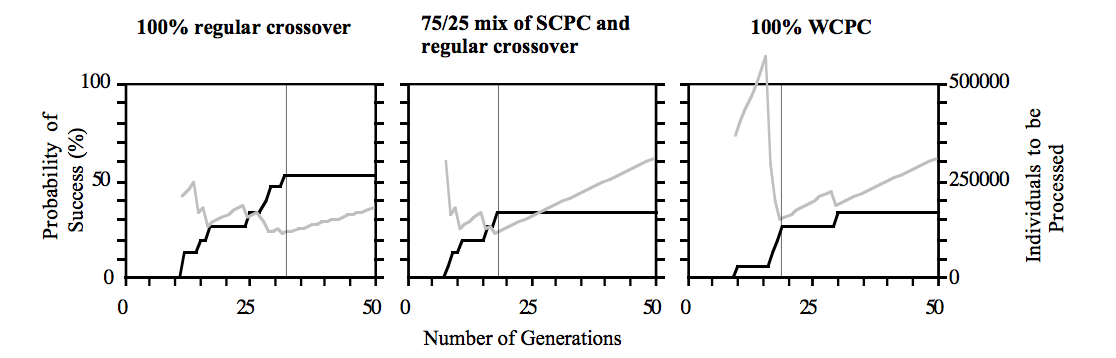
\includegraphics[scale=0.4]{./slike/ants.png}
	\caption{Učinkovitost različitih operatora križanja za problem centralnog sakupljališta hrane. lijevo: jednostavno križanje, sredina: kombinacija jednostavnog i križanja sa slabim očuvanjem konteksta, desno:  križanje s jakim očuvanjem konteksta}
	\label{ants}
\end{figure}



Ova istraživanja pokazala su kako križanje s očuvanjem konteksta nije učinkovito kada je upotrebljeno samo, već je efikasnije u kombinaciji s nekim drugim operatorom. Kombinacija jednostavnog križanja i križanja s jakim očuvanjem konteksta pokazala se kao vrlo učinkovit operator za iterirane programe koji predstavljaju neovisnu jedinku i za pronalazak logičkih funkcija.



\section{Križanje pravedno s obzirom na veličinu}
Česta pojava u genetskom programiranju je prekomjeran rast jedinki kako teku generacije (\textit{eng. bloat}). Postoji više načina rješavanja ili sprječavanja ovog problema. Jedan od načina kako riješiti ovaj problem nad već generiranim jedinkama je podrezivanje (\textit{eng. pruning}), odnosno odstranjivanje onih dijelova stabla koji su izvan dopuštene dubine. Drugi način je da se rezultat operatora križanja odbacuje sve dok je stablo producirano takvim križanjem veće dubine nego što je dopušteno. Moguće je i kažnjavati predugačka rješenja umanjivanjem njihove dobrote. Ovaj operator taj problem rješava u samom postupku križanja. Naime, kontrolirajući veličinu podstabala koja ulaze u križanje, direktno kontrolira veličinu novogeneriranog potomka.

Nakon što je algoritam dosegnuo stagnaciju u napredovanju, uobičajeni operatori križanja pokušat će proširiti prostor pretrage. No, radi pojave prekomjernog rasta, ova potraga više će se protezati u prostoru duljine samog rješenja nego u prostoru različitih rješenja. Kod ovakvog pristupa, postoji veća vjerojatnost za preživljavanjem dijelova rješenja koji nisu štetni, ali nisu ni korisni - podržavajući tako daljnji rast jedinki. Kod križanja pravednog s obzirom na veličinu, to nije slučaj - nakon dosegnutog platoa, ono će istraživati različita rješenja, čisto iz razloga što je jedinka dobivena ovakvim križanjem otprilike jednake veličine kao i svoji roditelji.

U \cite{crxSizeFair} predstavljeno je križanje pravedno s obzirom na veličinu. Odabir točke prekida u prvom roditelju koji sudjeluje u križanju obavlja se nasumično. Pri tome, pristranost odabiru nezavršnog čvora stabla nad odabirom lista stabla iznosi 0.9. Ono po čemu se ovo križanje razlikuje od jednostavnog križanja je odabir točke prekida u drugom roditelju. Kako bi se pronašla druga točka prekida, izračunava se veličina stabla koje će biti obrisano u kopiji prvog roditelja. Nakon toga, u drugom stablu pronalaze se podstabla veličine ne veće od $1+2 \cdot |veličina\_obrisanog\_podstabla|$. Ovime se osigurava da novostvorena jedinka neće biti veća od $veličina\_prvog\_roditelja + |veličina\_obrisanog\_podstabla| + 1$.



\subsection{Dosadašnji rezultati}
U \cite{crxSizeFair}  provedeno je istraživanje nad četiri različita problema; po dva za simboličku regresiju (polinomi petog i šestog stupnja) i po dva za logičke funkcije (6 i 11 - multipleksor). Pokazano je kako je ovaj operator križanja kroz generacije proizvodio značajno, pa čak i do deset puta manje jedinke nego jednostavni operator križanja. Uočeno je da je u slučaju kada se početna populacija sastoji od jedinki koje su puno manje nego što je potrebno, jednostavno križanje i dalje superiornije pri pronalasku rješenja. Ovo se može pokazati kao značajan nedostatak ukoliko se na početku algoritma ne poznaje okvirna veličina dobrog rješenja. Dokazano je da ovaj operator značajno smanjuje prekomjeran rast jedinki. Za usporedbu, prosječan rast jedinki tijekom generacija za jednostavno križanje je linearno, dok je prosječan rast jedinki za ovo križanje subkvadratno.

\section{Uniformno križanje}
Uniformno križanje predstavljeno je u \cite{crxUniform}. Inspirirano je uniformnim križanjem nestablastih struktura u genetskom algoritmu. U genetskom algoritmu, ovo križanje (budući da su sve jedinke jednakih dužina) prolazi kroz oba roditelja te na svakoj poziciji nasumično odabire gen iz prvog ili drugog roditelja te ga ugrađuje u dijete. Kada bi u genetskom programiranju sve jedinke bile potpuno jednakog oblika, ovo križanje funkcioniralo bi potpuno jednako. No, budući da je to vrlo rijedak slučaj, potrebno je, kao i u križanju s jednom točkom prekida, pronaći zajedničko područje dva roditelja. Nakon što je to područje pronađeno, s lakoćom se smiju izmjenjivati čvorovi roditeljskih stabala - no pritom je potrebno paziti na broj djece koji taj čvor posjeduje. Na slici \ref{crxUni} prikazan je primjer jednog mogućeg rezultata uniformnog križanja.

\begin{figure}[H]
 	\centering


\begin{tikzpicture}
	[sibling distance=25mm, level distance=15mm,
	every node/.style={fill=blue!20,circle,draw,drop shadow, minimum height=1cm}]

\begin{scope}[xshift=0cm]

	\node  [fill=yellow!20]  {\textbf{+}}
    		child {node [fill=yellow!20]  {$cos$}
    			child {node  [fill=yellow!20] {-}
    				child {node{x}}
    				child {node{y}}
    			}
    		}
    		child {node [fill=yellow!20]  {\textbf{$\cdot$}}
        		child {node [fill=yellow!20]  {2}}
        		child {node [fill=yellow!20]  {y}}
      		};
	};
\end{scope}

\begin{scope}[xshift=7cm]
	\node  [fill=yellow!20]  {\textbf{+}}
    		child {node  [fill=yellow!20] {$sin$}
        		child {node  [fill=yellow!20] {y}}
      		}
    		child {node [fill=yellow!20] {\textbf{$/$}}
			child {node [fill=yellow!20]  {x}}
			child {node [fill=yellow!20]  {y}}	
		};
	};
\end{scope}

\end{tikzpicture}


	\caption{Zajedničko područje dva roditelja}
	\label{crxOnePointCommon}
\end{figure}

\begin{figure}[H]
 	\centering


\begin{tikzpicture}
	[sibling distance=25mm, level distance=15mm,
	every node/.style={fill=blue!20,circle,draw,drop shadow, minimum height=1cm}]

\begin{scope}[xshift=0cm]

	\node {\textbf{+}}
    		child {node [fill=red!20]  {$sin$}
    				child {node{-}
    					child {node {x}}
    					child {node {y}}
    			}
    		}
    		child {node  [fill=red!20] {\textbf{$/$}}
        		child {node [fill=red!20]  {x}}
        		child {node {y}}
      		};
	};
\end{scope}

\begin{scope}[xshift=7cm]
	\node   {\textbf{+}}
    		child {node  [fill=red!20] {$sin$}
        		child {node  [fill=red!20] {y}}
      		}
    		child {node  [fill=red!20]  {\textbf{$\cdot$}}
			child {node  {x}}
			child {node  {y}}	
		};
	};
\end{scope}

\end{tikzpicture}


	\caption{Mogući rezultati križanja roditelja sa slike \ref{crxOnePointCommon}}
	\label{crxUni}
\end{figure}

Velika prednost ovog križanja je velika stopa razmjene genetskog materijala. Budući da se čvorovi koji će završiti u djetetu biraju uniformno, s omjerima vjerojatnosti 1:1, velika je vjerojatnost da će dijete sadržavati 50\% genetskog materijala prvog roditelja i 50\% genetskog materijala drugog roditelja. Ovo je vrlo pogodno za brzo napredovanje algoritma.

\subsection{Dosadašnji rezultati}
Autor ovog križanja proveo je eksperimente nad paritetnim problemom 4 varijable. Cilj ovog problema je pronaći logičku funkciju koja je istinita za parni broj istinitih varijabli. Tablica istinitosti za ovaj problem prikazana je na tablici ispod (\ref{truthTable}).

\begin{table}[H]
\centering

\begin{tabular} {a b c d | p}
A & B & C & D & P \\
\hline
0 & 0 & 0 & 0 & 1 \\
0 & 0 & 0 & 1 & 0 \\
0 & 0 & 1 & 0 & 0 \\
0 & 0 & 1 & 1 & 1 \\
0 & 1 & 0 & 0 & 0 \\
0 & 1 & 0 & 1 & 1 \\
0 & 1 & 1 & 0 & 1 \\
0 & 1 & 1 & 1 & 0 \\
1 & 0 & 0 & 0 & 0 \\
1 & 0 & 0 & 1 & 1 \\
1 & 0 & 1 & 0 & 1 \\
1 & 0 & 1 & 1 & 0 \\
1 & 1 & 0 & 0 & 1 \\
1 & 1 & 0 & 1 & 0 \\
1 & 1 & 1 & 0 & 0 \\
1 & 1 & 1 & 1 & 1 \\
\hline
\end{tabular}

	\caption{Tablica istinitosti za paritetni problem 4 varijable}
	\label{truthTable}
\end{table}

Eksperimentima je dokazano kako za razliku od jednostavnog križanja i križanja s jednom točkom prekida, u kojima je prosječna stopa razmjene genetskog materijala oko 5\%, ovo križanje uistinu ima konstantnu stopu razmjene genetskog materijala od oko 50\%.

Pokazano je kako jednostavno križanje pretragu prostora rješenja odvija lokalno, nasljeđujući većinu genetskog materijala od jednog roditelja. Jednostavno križanje nije idealno za brzo pretraživanje prostora - bolje je za fino ugođavanje prilično dobrog rješenja. Osim toga, jednostavno križanje vrlo lako zapne u nekom od lokalnih optimuma. 

Križanje s jednom točkom prekida bolje se nosi s veličinom prostora pretrage, no nakon nekog vremena počinje sagledavati sve manji dio prostora - lokalizirajući tako pretragu s povećanjem vjerojatnosti zapinjanja u lokalnom optimumu.

Uniformno križanje prelazi preko ovih problema. Za razliku od jednostavnog križanja, ono nije pristrano na križanje listova ili podstabala. Ovime omogućuje slobodniju i raznolikiju izmjenu genetskog materijala između roditelja, ubrzavajući tako konvergenciju rješenja u globalni optimum. Također, pokazano je kako nakon nekog vremena, sve jednike populacije budu otprilike jednake veličine, što kod upotrebe jednostavnog križanja i križanja s jednom točkom prekida nije slučaj. Osim navedenih svojstava, nije uočena prevelika razlika u samoj uspješnosti križanja da pronađe dobro rješenje problema - rad se pretežito fokusirao na razliku u količini izmijenjenog genetskog materijala.



\section{Homologno križanje}
Homologno križanje \cite{crxSizeFair} temelji se na prirodnom svojstvu križanja, homologiji. Homologija u prirodi osigurava da se križanje uvijek događa između organizama koji imaju uglavnom identične sekvence gena unutar kromosoma. Ovime se podupire nedestruktivno križanje - kombiniraju se geni koji rade točno određenu ulogu, gdje je uloga uvjetovana pozicijom samog gena.

Homologno križanje, u smislu križanja u genetskom programiranju, koristi pozicijsku homologiju. Pozicijska homologija potiče izmjenu genetskog materijala samo ako se ono događa na istoj, ili dovoljno bliskoj poziciji unutar dva genoma.

Uobičajeni operatori križanja, prilikom odabira podstabala ili čvorova koji sudjeluju u križanju uglavnom ne uzimaju u obzir njihovu poziciju. Ne uzimajući to u obzir, nerijetko dolazi do naglog rasta jedinki svakom novom generacijom (\textit{eng. bloat}). Budući da ovi operatori najčešće ne uzimaju u obzir prekomjeran rast jedinki koje proizvode, potrebno je modificirati sam algoritam tako da se prevelike jedinke kažnjavaju manjom dobrotom. Time, iako možda novonastala jedinka izvrsno rješava zadan problem, može se dogoditi da bude odbačena zbog svoje veličine. Iz razloga što se ne uzimaju u obzir pozicije niti veličine podstabala koja sudjeluju u križanju, mala je šansa da će novonastala jedinka biti u okviru željene veličine, povećavajući šansu da će u budućnosti zbog te veličine i izumrijeti. Drugi razlog zbog kojega prekomjeran rast jedinke nije dobar, a usko je povezan s prethodnim, je taj da, u prevelikoj jedinci vjerojatno postoji puno nepotrebnog ponašanja - ponašanje koje nije potrebno, a kroz generacije je preživjelo samo zato što ne donosi nikakvu štetu.

Drugi problem koji se javlja kod uobičajenih operatora križanja je taj da ti operatori potpuno nasumično prenose dijelove programa u novu jedinku. Budući da je taj fragment jedinke preživio proces selekcije, za pretpostaviti je da postoji velika šansa da on predstavlja relevantan dio za put do konačnog rješenja. Također, velika je šansa da korisnost istog fragmenta uvelike ovisi i o kontekstu u kojem se on izvršava. Stavljajući takav fragment na nasumično mjesto u novu jedinku donosi šansu da će taj kontekst biti uništen.

Kako bi se ovi problemi riješili prilikom samog križanja, a time se i povećale šanse za kvalitetu i nastavak života potomaka, homologni operator križanja prilikom samog križanja uzima u obzir i veličinu i poziciju podstabala roditelja koja će se iskrižati. Ovime se u samoj srži operatora sprječava prekomjeran rast potomaka i s većom vjerojatnošću nego inače, podržava prijenos konteksta pojedinih fragmenata rješenja u ono novonastalo.

Ovo križanje u stvari je inačica križanja pravednog s obzirom na veličinu. Odabir potencijalnih podstabala drugog roditelja potpuno je jednak u ovom križanju kao i kod križanja pravednog s obzirom na veličinu. Razlika u tome je ta da se, između svih potencijalnih podstabala drugog roditelja koji bi mogli sudjelovati u križanju, odabire ono podstablo koje je najbliže točki prekida prvog roditelja. Na slici \ref{crxHomo} prikazan je jedan takav primjer križanja - od dva potencijalna podstabala drugog roditelja, za križanje je odabrano ono koje je bliže točki prekida u prvom roditelju.

\begin{figure}[H]
	\centering
	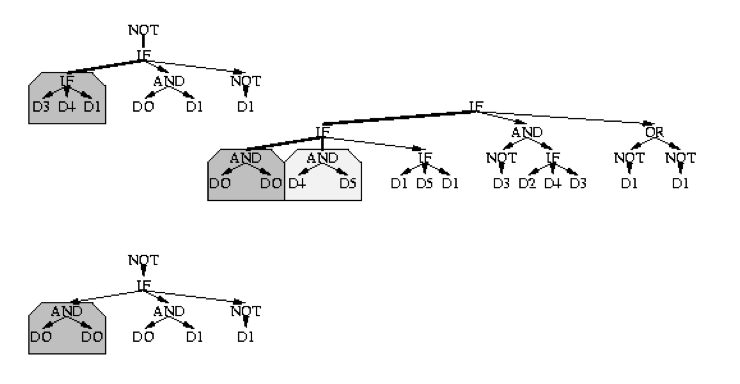
\includegraphics[scale=0.6]{./slike/crxHomo.png}
	\caption{Primjer homolognog križanja (preuzeto iz  \cite{crxSizeFair})}
	\label{crxHomo}
\end{figure}

\subsection{Dosadašnji rezultati}
U \cite{crxSizeFair}  provedeno je istraživanje nad četiri različita problema; po dva za simboličku regresiju (polinomi petog i šestog stupnja) i po dva za logičke funkcije (6 i 11 - multipleksor). Pokazano je kako homologno križanje po sposobnosti pronalaska rješenja danih problema nije značajno bolje od križanja pravednog s obzirom na veličinu. No, kao i kod križanja pravednog s obzirom na veličinu, pokazano je kako je ovo križanje vrlo učinkovito prilikom sprječavanja pojave prekomjernog rasta jedinki.

Razlog sličnosti u rezultatima s križanjem pravednim s obzirom na veličini može biti prouzrokovano različitim razlozima. Jedan od razloga je mogućnost da kod ovog operatora u nekim slučajevima nije postojao izbor podstabla koji bi bio u skladu s homologijom, te bi operator bio primoran odabrati podstablo koje ne odgovara u potpunosti načelu odabira. Postojanje ovog slučaja pokazano je u spomenutom radu.



\section{Determinističko križanje}
Determinističko križanje (\textit{eng. deterministic functional crossover}), opisano u \cite{crxDeter}, ostvaruje križanje dvije jedinke na osnovi funkcijske sličnosti. Ovaj operator primjenjiv je samo na probleme simboličke regresije.

Kako bi se funkcijska sličnost dva gena, odnosno čvorova stabla koji izgrađuju jedinku, mogla odrediti, za svaki gen zapisuje se minimalna i maksimalna vrijednost koju može poprimiti za podatke iz skupa za učenje. Funkcijska sličnost (u radu nazvana funkcijskom udaljenošću) između dva gena i i j, računa se kao:

\begin{equation} 
\label{udaljenost}
 \large{ d_{i,j} = \frac{1}{2} (|max_i - max_j| + |min_i - min_j|) }
\end{equation}
\\
U radu je opisan glavni nedostatak ovog križanja - postoji velika vjerojatnost da križanje koje se dogodi pod utjecajem ovog operatora bude neutralno, odnosno, da se novonastala jedinka uopće ne razlikuje od jednog od roditelja. Ovaj slučaj dogodi se kada se u prvom roditelju izabere podstablo koje je strukturno jednako odabranom podstablu drugog roditelja (može biti interpretirano na jednak način nakon što se izraz predstavljen podstablom simplificira). Križanjem takvih podstabala, originalno ponašanje se uopće ne mijenja te je rezultantna jedinka potpuno jednaka svome roditelju. Pojava neutralnog križanja to je češća što jedinke sve više i više rastu (čime se povećava vjerojatnost odabira strukturno jednakog podstabla). Kako bi se riješio ovaj problem, u istom radu predloženo je probabilističko križanje, koje je opisano u idućem poglavlju.

\subsection{Dosadašnji rezultati}
Na slici \ref{deto} prikazani su grafovi usporedbe učinkovitost determinističkog križanja u usporedbi s jednostavnim i probabilističkim križanjem i slučaja kada nije upotrijebljen niti jedan operator križanja. Pri tome, grafovi na lijevoj strani pokazuju performanse dobivenih rješenja na skupu za učenje, a oni na desnoj strani, performanse na skupu za testiranje. Eksperimenti su bili provedeni na primjerima simboličke regresije. Na desnoj strani slike, vidljivo je kako ne postoji prevelika razlika između učinkovitosti danih operatora. 


\begin{figure}[H]
	\centering
	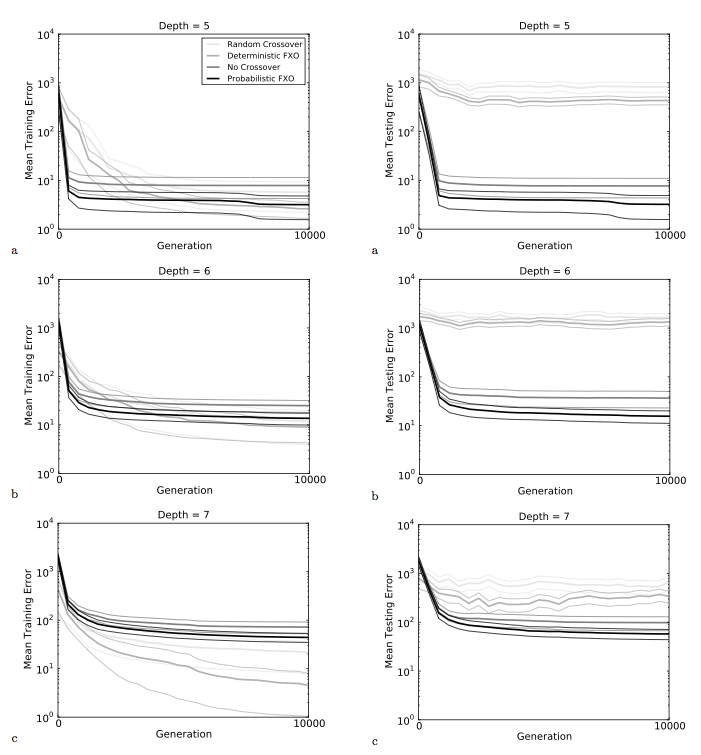
\includegraphics[scale=0.65]{./slike/deto.png}
	\caption{Usporedba učinkovitosti determinističkog, jednostavnog i probabilističkog križanja i slučaja kada nije upotrijebljen niti jedan operator križanja (preuzeto iz \cite{crxDeter})}
	\label{deto}
\end{figure}

Također, vidljivo je kako je ovo križanje dalo superiorno rješenje na skupu za učenje naspram ostalima za slučaj kada je dubina stabla jednaka 7. U suprotnosti, odnosno, posljedično tome, na skupu za testiranje isti slučaj dao je značajno slabije rezultate što upućuje na prenaučavanje jedinki.

Također, pokazano je da ovo križanje ne podržava prekomjeran rast jedinki tijekom generacije. Dapače, dana rješenja često su ispala nešto manja od onog ciljanog.




\section{Probabilističko križanje}

Kako bi se riješio problem neutralnog križanja koji se pojavio kod determinističkog križanja, u \cite{crxDeter} je predloženo probabilističko križanje (\textit{eng. probabilistic functional crossover}). Jednako kao i kod determinističkog križanja, za svaki čvor u stablu zapisuje se minimalna i maksimalna vrijednost čvora za podatke iz skupa za učenje (izraz \ref{udaljenost}).

Prilikom križanja, nakon što se u prvom stablu nasumično odabere točka križanja izračunava se funkcionalna udaljenost između njega i svakog čvora unutar drugog roditelja (jednako kao i kod determinističkog križanja). Nakon što su dobivene sve moguće udaljenosti, one se normaliziraju prema \ref{norm}:

\begin{equation} 
\label{norm}
 \large{ d '_{i,j} = \frac{d_{i,j}}{\sum_{k=1}^{s} d_{i,k}} }
\end{equation}
 
Normalizacija je pogodna iz razloga što se s najvećom vjerojatnošću želi odabrati funkcionalno najbliži čvor. Ovako dobivene normalizirane udaljenosti potom se invertiraju i ponovno normaliziraju u odnosu na te invertirane vrijednosti prema \ref{prob}:
 
 \begin{equation} 
\label{prob}
 \large{ p_{i,j} = \frac{1 - d '_{i,j}}{\sum_{k=1}^{s} (1 - d '_{i,k})} }
\end{equation}

Time dobivamo to veću vjerojatnost što je udaljenost između dva čvora manja. Nakon ovih operacija, nasumično, ali s izračunatim vjerojatnostima, odabire se podstablo unutar drugog roditelja koje će se iskoristiti za križanje. Pokazano je kako ovakvo križanje pridonosi većem postotku korisnog križanja, a time i bržoj konvergenciji nego uobičajeni operatori, iako je priznato kako je ovakav izračun udaljenosti prilično gruba aproksimacija funkcionalne udaljenosti.

\subsection{Dosadašnji rezultati}
Jednako kao i za determinističko križanje, provedeni eksperimenti za ovo križanje uključuju usporedbu probabilističkog, determinističkog i jednostavnog križanja i slučaja kada nije upotrijebljen niti jedan operator križanja. Rezultati su prikazani su na slici \ref{deto}. Vidljivo je kako probabilističko križanje konstantno bolje djeluje od jednostavnog križanja i slučaja kada se ne koristi niti jedan operator križanja.

Osim toga, dokazano je kako je korisnost križanja \footnote{križanje se smatra korisnim ukoliko producira jedinku koja ima dobrotu bolju od oba roditelja}, kada se koristi probabilistički operator križanja, puno veća nego u ostalim slučajevima. Pokazano je kako se ovim križanjem dobivaju jedinke koje su značajno veće od točnog rješenja. Naravno, pitanje je kako interpretirati ovu pojavu, budući da se izraz koji predstavlja jedinka gotovo uvijek može pojednostavniti čime bi stablo bilo puno manje.

Uočena je korelacija između veličine roditelja i događanja korisnog križanja. No, to je i za očekivati iz razloga što je omjer broja listova na prema unutarnjim čvorovima to veći što je samo stablo veće. Radi toga, vjerojatnost odabira lista za ulazak u križanje se povećava, čime se i smanjuje mogućnost za destruktivnim križanjem. 

\section{Semantičko križanje}
Suprotstavljeno tradicionalnim operatorima križanja u genetskom programiranju koji ignoriraju semantiku samog programa, u \cite{crxSem} opisano je semantičko križanje. 
Ovo križanje razlikuje nekoliko inačica, od kojih je svaka primjenjiva na određenu vrstu problema. Semantičko križanje različito je definirano za situacije kada stablo jedinke predstavlja logičku ili realnu funkciju, ili ako je jedinka program.

Ukoliko jedinka predstavlja logičku funkciju, semantičko križanje definirano je kao:
 \begin{equation} 
\label{log}
 \large{ (T1 \land T2) \vee   (\overline{TR} \land T2) },
\end{equation}
gdje T1 i T2 predstavljaju roditelje koji sudjeluju u križanju, a TR predstavlja nasumično generirano stablo. Na slici \ref{semBool} prikazana je shema semantičkog križanja za logičke funckije.

 \begin{figure}[H]
	\centering
	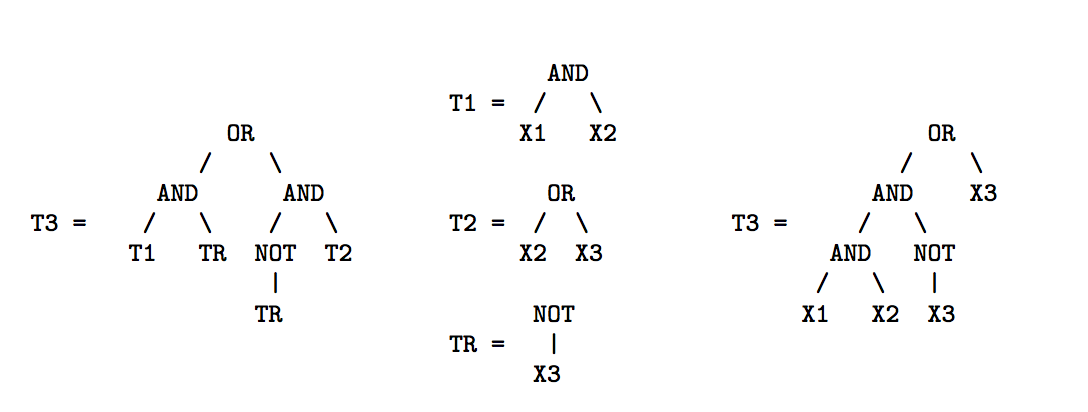
\includegraphics[scale=0.4]{./slike/semBool1.png}
	\caption{Lijevo: shema semantičkog križanja za logičke funkcije; sredina: roditelji i nasumično generirana jedinka; desno: rezultat križanja roditelja prikazanih u sredini }
	\label{semBool}
\end{figure}
  
   
     Analogno ovome, za realne funkcije, odnosno, simboličku regresiju, semantičko križanje predstavljeno je sljedećim izrazom:
 \begin{equation} 
\label{log}
 \large{ (T1 \cdot T2) +   ((1-TR) \cdot T2) }.
\end{equation}
Za slučaj kada jedinka predstavlja program, semantičko križanje definira se kao:
 \begin{equation} 
\label{log}
 \large{ \textbf{IF}(CONDR) \textbf{THEN} (T1) \textbf{ELSE} (T2)},
\end{equation}
gdje je CONDR nasumično generiran program čiji je izlaz interpretiran kao logička vrijednost.

Iz ovoga je jasno vidljiv najveći nedostatak ovog operatora - prekomjeran rast novonastalih jedinki. Naime, prilikom svakog križanja stablo će se sigurno uvećati po dubini za barem jednu razinu. Ovo može postati znatan problem iz razloga što je rast vrlo brz, te se često nakon nekog vremena dogodi to da za novodobiveno stablo ne postoji prostor za pohranu. Radi ovoga, nakon svakog križanja, potrebno je pojednostavniti novonastalu jedinku. Ovo pojednostavljenje naravno mora osigurati da je funkcionalnost jedinke nakon pojednostavljenja ostala nepromijenjena.

Glavna prednost ovog semantičkog operatora je činjenica da je, za razliku od nekih drugih predloženih semantičkih operatora, primjenjiv na širok skup problema.

\subsection{Dosadašnji rezultati}

Eksperimenti u \cite{crxSem} provedeni su nad sve tri vrste problema za koje je ovaj operator definiran; logičke funkcije, simboličku regresiju i programe. Ovo istraživanje je usporedilo genetsko programiranje (\texit{GP}) sa semantičkim genetskim programiranjem (\textit{eng. semantic genetic programming - SGP}) i semantičkim stohastičkim planinskim penjačem (\textit{semantic stochastic hill climber - SSHC}). Također, napravljena je usporedba s algoritmom genetskog programiranja koje se vrti jednako dugo kao i SGP i SSHC za pojedini problem (\textit{GPt}). U nastavku su opisani dobiveni rezultati za pojedinu vrstu problema.

\subsubsection{Logičke funkcije}

Učinkovitost logičkog semantičkog operatora križanja provedena je na 5 različita problema, zajedno s nekoliko inačica za svaki problem. Problemi su redom: $n$ -komparator (6, 8 i 10), $n$ -multipleksor (6 i 11), $n$ -paritet (5, 6, 7, 8, 9 i 10), nasumično generirana funkcija $n$ varijabli (5, 6, 7, 8, 9, 10 i 11) i $n$-istinita funkcija \footnote{$n$-istinita funkcija je funkcija $n$ varijabli koja je za svaku kombinaciju varijabli istinita} (5, 6, 7 i 8). Dobrota je računata kao Hammingova udaljenost vrijednosti stvarne funkcije i dobivenog rješenja. Na slici \ref{semBoolTable} prikazana je tablica rezultata. 

Stupac \textit{Hits \%} predstavlja postotak uspješnosti nad skupom za učenje za najbolju jedinku u populaciji, za 30 pokretanja algoritma. Pri tome \textit{avg} predstavlja prosjek, a \textit{sd} standardnu devijaciju. U stupcu \textit{Length} prikazani su logaritmi po bazi 10 veličine dobivenih rješenja. Valja napomenuti da je nakon upotrebe semantičkog križanja primijenjena simplifikacija dobivenog rješenja, iz razloga što bi veličina rješenja eksponencijalno rasla u suprotnom. Vidljivo je kako SSHC i SGP konstantno pronalaze bolja rješenja od GP-a sa semantičkim križanjem, no GP proizvodi manje jedinke (čemu je glavni razlog pojednostavljenje izraza koje se u ostalim algoritmima ne obavlja - što umanjuje relevantnost ovog zaključka).  Vidljivo je kako GPt pokazuje bolje performanse od GP-a, no još uvijek se pokazuje lošijim od SGP-a i SSHC-a.

 \begin{figure}[H]
	\centering
	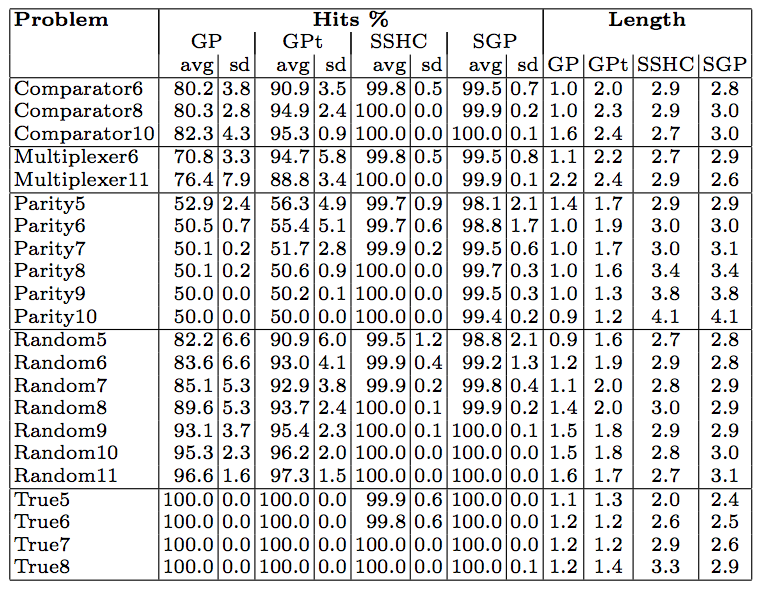
\includegraphics[scale=0.5]{./slike/semBoolTable.png}
	\caption{Usporedba učinkovitosti GP-a i GPt-a sa SGP-om i SSHC-om}
	\label{semBoolTable}
\end{figure}

\subsubsection{Simbolička regresija}

Za ocjenu učinkovitosti ovog operatora na simboličkoj regresiji korišteni su različiti polinomi, od trećeg do desetog stupnja, s koeficijentima realnih vrijednosti iz intervala $[-1, 1]$. Funkcija dobrote računata je kao euklidska udaljenost stvarne funkcije i pronađenog rješenja. Na slici \ref{semSymbTable} prikazane su dobivene statistike provedenih eksperimenata.

 \begin{figure}[H]
	\centering
	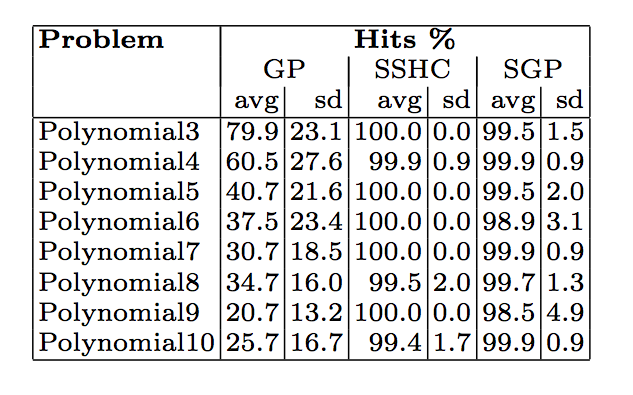
\includegraphics[scale=0.4]{./slike/semSymbTable.png}
	\caption{Usporedba učinkovitosti GP-a i GPt-a sa SGP-om i SSHC-om}
	\label{semSymbTable}
\end{figure}

Vidljivo je kako je GP kao i u prethodnom slučaju, gori od SSHC-a i SGP-a, te da je standardna devijacija dosta veća nego kod ostalih.

\subsubsection{Programi}

Kako bi se pokazala učinkovitost semantičkog križanja nad programskim jedinkama, korišten je problem klasifikacije u jednu klasu na osnovu dvije značajke ($(n_c, n_v) \to n_ {cl}$). Na slici \ref{semProg} prikazani su rezultati eksperimenata. Ovdje je ponovno pokazana inferiornost GP-a naprema SSHC-u i SGP-u.

 \begin{figure}[H]
	\centering
	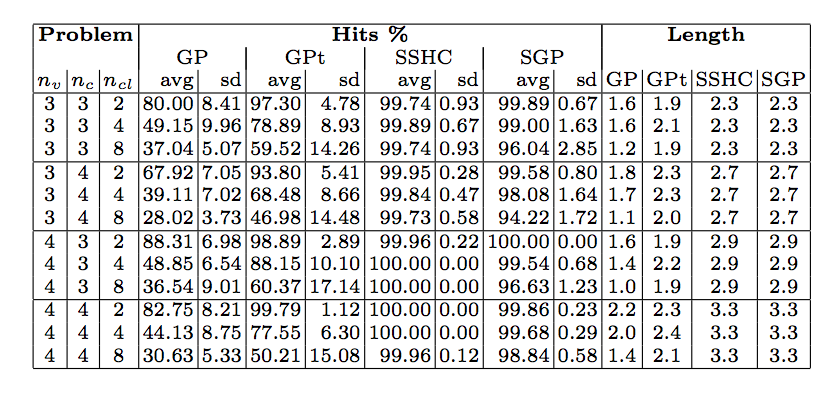
\includegraphics[scale=0.5]{./slike/semProg.png}
	\caption{Usporedba učinkovitosti GP-a i GPt-a sa SGP-om i SSHC-om}
	\label{semProg}
\end{figure}

Unatoč prikazanim rezultatima, autori \cite{crxSem} tvrde da ovaj operator križanja djeluje bolje od uobičajenih operatora u genetskom programiranju. No, za to nisu priložili nikakav dokaz. U sklopu ovog rada implementirano je ovakvo križanje, te će u kasnijim poglavljima biti prikazana usporedba učinkovitosti ovog operatora s onim operatorima koji su opisani u prethodnim poglavljima.

\section{Tablica primjenjivosti operatora na različite vrste problema}
U tablici \ref{crxtable} prikazana je primjenjivost operatora na različite vrste problema genetskog programiranja. 

\begin{table}[H]
 	\centering

    \caption{Tablica primjenjivosti operatora na različite vrste problema}
    \begin{tabular}{| l | l | l | l |}
    \hline
    \textbf{operator - primjenjiv na} & \textbf{logičke funkcije} & \textbf{simbolička regresija} & \textbf{programi}\\ \hline
    jednostavno & da & da & da\\ \hline
    s jednom točkom prekida & da & da & da\\ \hline
    s očuvanjem konteksta  & da & da & da\\ \hline
    pravedno s obzirom na veličinu  & da & da & da\\ \hline
    uniformno  & da & da & da\\\hline
    homologno  & da & da & da\\ \hline
    determinističko & ne & da & ne\\ \hline
    probabilističko  & ne & da & ne\\ \hline
    semantičko  & da & da & da\\ \hline
    \end{tabular}
    \label{crxtable}
\end{table}

\chapter{Ispitivanja}
U ovom poglavlju biti će opisana istraživanja provedena u sklopu ovog rada. Za istraživanja je korišteno radno okruženje ECF (\textit{eng. Evolutionary Computation Framework}) koje je za potrebe ovog rada nadograđeno potrebnim, nedostajućim  operatorima križanja.

\section{ECF}
ECF \cite{ecf} (\textit{eng. Evolutionary Computation Framework}) predstavlja okruženje napisano u jeziku C++ za rješavanje različitih problema evolucijskog računanja. Za potrebe ovog rada, najznačajnije korišten dio ECF-a uključuje stablasti genotip (\textit{eng. tree}), zajedno s njegovim operatorima križanja i mutacije. Dio koji je nedostajao ovom okruženju za provedbu kasnije opisanih eksperimenata uključuje implementaciju homolognog, determinističkog, probabilističkog i semantičkog križanja. Iz tog razloga, kao praktičan dio ovog rada, ECF je nadograđen sa spomenutim operatorima križanja.

\section{Problemi za ispitivanje}

Kako bi se pokazala učinkovitost različitih operatora križanja nad različitim vrstama problema, ispitivanja su provedena nad različitim problemima simboličke regresije i logičke i programske domene. U nastavku je za svaku vrstu problema opisan specifičan problem koji je kasnije korišten za provedbu istraživanja. Nakon toga dana je detaljna analiza dobivenih rezultata, koja sadrži međusobnu usporedbu učinkovitosti različitih operatora križanja za svaki pojedini problem.

\subsection{Logičke funkcije}

\subsubsection{Multipleksor problem}
Kako bi se ispitala učinkovitost operatora križanja nad evolucijom logičkih funkcija, provedeni su eksperimenti nad 6 - multipleksor i 11 - multipleksor problemu \cite{koza}. Općenito, cilj $n$ - multipleksor problema je pronaći logičku funkciju koja za danih $n$ bitova (od kojih je određen broj adresnih i podatkovnih bitova) generira odgovarajući ulaz. Na slici \ref{muxPicture} prikazan je 6 - multipleksor, koji za 2 adresna bita na izlaz propušta jedan od 4 podatkovna bita.

\begin{figure}[H]
\centering

\begin{tikzpicture}
  % Inputs
  \draw[|-o] (-2,3.5) node[anchor=east] {$d_0$} -- (0.5,3.5);
  \draw[|-o] (-2,2.5) node[anchor=east] {$d_1$} -- (0.5,2.5);
  \draw[|-o] (-2,1.5) node[anchor=east] {$d_2$} -- (0.5,1.5);
  \draw[|-o] (-2,0.5) node[anchor=east] {$d_3$} -- (0.5,0.5);

  % Output
  \draw[o-|] (2.75,2) -- (5.25,2) node[anchor=west] {$y$};

  % Select
  \draw[|-o] (1,6) node[anchor=south] {$a_0$} -- (1,3.5);
  \draw[|-o] (2,6) node[anchor=south] {$a_1$} -- (2,3.5);

  % Rectangle
  \draw (0,0) rectangle node {Multipleksor} (3,4);

\end{tikzpicture}

\caption{6 - multipleksor}
  \label{muxPicture}
\end{figure}

Primjerice, za adresne bitove $a_0=1$ i $a_1=0$, na izlaz bi se pustio drugi po redu podatkovni bit (01 binarno = 1 decimalno), odnosno $d_1$.

U tablici \ref{muxTable} prikazani su korišteni parametri za predstavljene 6 i 11 - multipleksor probleme.

\begin{table}[H]
 	\centering
    \caption{Parametri $n$ multipleksor problema}
    \begin{tabular}{| l | l | l |}
    \hline
   problem & 6 - multipleksor & 11 - multipleksor \\ \hline
   skup završnih znakova & $\{a_0, a_1, d_0, d_1, d_2, d_3 \}$ & $\{a_0, a_1, a_2, d_0, d_1, d_2, d_3, d_4, d_5, d_6, d_7 \}$\\ \hline
   skup nezavršnih znakova & $\{ AND, OR, NOT, IF \}$  & $\{ AND, OR, NOT, IF \}$ \\ \hline
   funkcija dobrote & broj netočnih izlaza & broj netočnih izlaza \\ \hline
    \end{tabular}
    

    \label{muxTable}
\end{table}

\subsubsection{Evolucija kriptografski sigurnih logičkih funkcija}
Za ispitivanje učinkovitosti operatora nad logičkim funkcijama također je korišten problem evolucije kriptografski sigurnih logičkih funkcija \cite{bool}. Cilj je pronaći neku logičku funkciju koja će imati dobra kriptografska svojstva. Svojstva koja posjeduje dobra kriptografska logička funkcija uključuju:

\begin{itemize}
\item{balansiranost - funkcija je balansirana ako ima jednak broj istinitih i lažnih vrijednosti}
\item{visoku nelinearnost - linearnost logičke funkcije definira se kao postojanje $a_0,a_1,...,a_n \in \{0, 1\}$ tako da je $f(b_1,...,b_n) =  a_0 \oplus (a_1 \wedge b_1) \oplus ... \oplus (a_n \wedge b_n)$ za sve $b_1,....,b_n \in \{0, 1\}$}
\item{visok algebarski stupanj - algebarski stupanj logičke funkcije jednak je broju varijabli izraza s najvećim brojem varijabli u algebarskom normalnom obliku funkcije}
\item{visok algebarski imunitet - algebarski imunitet definiran je kao minimalni broj ne-nul funkcija $g$ takvih da su $fg = 0$ ili $(f\oplus 1)g=0$}
\item{visok korelacijski imunitet - korelacijski imunitet funkcije $f$ je maksimalna vrijednost $m$ takva da $| F\^(\omega) |= 0$ za sve vrijednosti Hammingove težine $\omega \leq m$ }
\end{itemize}

Budući da je nemoguće stvoriti logičku funkciju koja posjeduje sva ova svojstva, algoritmu se postavlja zadatak pronalaska dobre kombinacije nekih od ovih svojstava.

\subsection{Simbolička regresija}

\subsubsection{Klasična simbolička regresija}
Simbolička regresija je postupak pronalaženja matematičkog izraza iz danih empirijskih podataka. Za potrebe ovih mjerenja korištena je stablasta jedinka koja predstavlja jedan matematički izraz. Taj izraz se iz jedinke može jednostavno iščitati \textit{in-order} obilaskom stabla. Na slici \ref{symbTree} prikazana je jedinka koja predstavlja matematički izraz $cos(x-y) + (x / y)$.

\begin{figure}[H]
 	\centering

\begin{tikzpicture}
	[sibling distance=25mm, level distance=15mm,
	every node/.style={fill=blue!20,circle,draw,drop shadow, minimum height=1cm}]

	\node   {\textbf{+}}
    		child {node {$cos$}
    			child {node {-}
    				child {node {x}}
    				child {node {y}}
    			}
    		}
    		child {node {\textbf{$/$}}
			child {node  {x}}
			child {node  {y}}	
		};
	};

\end{tikzpicture}


	\caption{Primjer jedinke koja rješava problem simboličke regresije koja predstavlja izraz $cos(x-y) + (x / y)$}
	\label{symbTree}
\end{figure}

U tablici \ref{bla} \footnote{mse označava kvadratnu sumu odstupanja (\textit{eng. mean square error})} su dani izrazi koji su bili ciljna funkcija u provedenim istraživanjima, zajedno s njihovim intervalom domene i oznakama koje su kasnije korištene za jednostavnije referenciranje.

\begin{table}[H]
 	\centering
 \caption{Popis problema simboličke regresije}
    \begin{tabular}{| l | l | l | l |}
    \hline
    oznaka & izraz & interval domene & funkcija dobrote\\ \hline
    symb1 & $log(x+1)+log(x^2+1)$ & $x \in [0, 20]$ & $mse$ \\ \hline
    symb2 & $sin(x) + sin(y^2)$ & $x, y \in [-10, 10]$ & $mse$\\ \hline
    symb3 & $2 \cdot sin(x) \cdot cos(y)$ & $x, y \in [-10, 10]$ & $mse$\\ \hline
    symb4 & $x \cdot y + sin((x+1) \cdot (y-1))$ & $x, y \in [-10, 10]$ & $mse$\\ \hline
    symb5 & \Large{ $\frac{8}{2 + x^2 + y^2}$ }& $x, y \in [-10, 10]$ & $mse$\\ \hline
    symb6 & $\frac{x^3}{5} + \frac{y^3}{2} - x - y$ & $x, y \in [-10, 10]$ & $mse$\\ \hline
    \end{tabular}
    
   
    \label{bla}
\end{table}

\subsubsection{Evolucija funkcije prioriteta za uporabu unutar pravila raspoređivanja}
Cilj ovog problema jest pronaći funkciju prioriteta koja će se upotrijebiti unutar pravila raspoređivanja \cite{jakobovic}. Pritom, pravila već imaju predefiniranu globalnu strukturu, dok se pojedini dijelovi evoluiraju genetskim programiranjem. Postupak raspoređivanja kojega algoritmi koriste je prioritetno raspoređivanje (\textit{engl. priority scheduling}), pri kojemu se zadano trenutno stanje sustava preslikava u sljedeće stanje. Prijelaz iz jednoga u drugo stanje definiran je pridruživanjem određene aktivnosti nekome sredstvu, a odabir aktivnosti i sredstva obavlja se računanjem prioriteta svakog raspoloživog sredstva i aktivnosti, ovisno o dotičnom okruženju. Ovisno o kriteriju raspoređivanja, funkcija prioriteta se pronalazi automatski, uz pomoć genetskog programiranja.


\subsection{Programi}
Programski problem korišten za evaluaciju operatora križanja bio je problem umjetnog mrava (\textit{eng. Artificial Ant Problem}). Rješenje ovog problema jest evoluirati program koji opisuje ponašanje mrava u nekoj okolini koja sadrži hranu. Dobar program bi trebao biti sposoban pronaći i pojesti što više hrane iz okoline. Jedinka je u ovom slučaju također predstavljena kao stablo. Primjer jedinke prikazan je na slici \ref{ant}. Dobrota jedne ovakve jedinke jednaka je broju pojedene hrane u ispitnoj, prilikom učenja neviđenoj okolini.

\begin{figure}[H]
	\centering

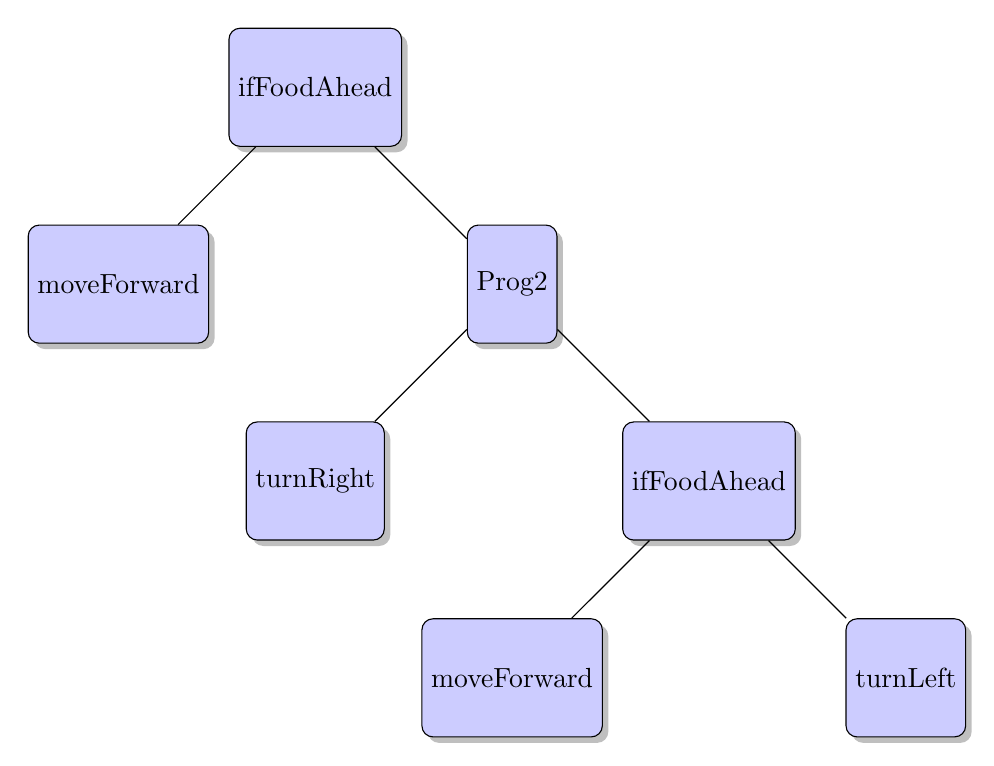
\begin{tikzpicture}
[sibling distance=50mm, level distance=25mm,
every node/.style={fill=blue!20,rectangle, rounded corners,draw,drop shadow, minimum height=1.5cm}]


  \node {ifFoodAhead}
      child {node {moveForward}}
      child {node {Prog2}
        child {node {turnRight}}
        child {node {ifFoodAhead}
        	child{node {moveForward}}
        	child{node {turnLeft}}
        }
      };
\end{tikzpicture}

	\caption{Primjer jedinke programa umjetnog mrava}
	\label{ant}
\end{figure}

Nezavršni znakovi koji grade jednu ovakvu jedinku su:

\begin{enumerate}

  \item \textbf{If food ahead} - provjerava da li se nalazi hrana ispred mrava - ako da izvršava lijevu granu, ako ne, izvršava desnu granu.
  \item \textbf{Prog2} - slijedno izvršava lijevu, te zatim desnu granu.
  \item \textbf{Prog3} - slijedno izvršava (s lijeva na desno) svaku od 3 pridružene grane.

\end{enumerate}

Završni znakovi koji grade ovu jedinku su:
\begin{enumerate}

  \item \textbf{move forward} - pomiče mrava za jedno mjesto unaprijed.
  \item \textbf{turn right} - okreće mrava u desno.
  \item \textbf{turn left} - okreće mrava u lijevo.

\end{enumerate}


\section{Rezultati}

U ovom poglavlju dan je pregled provedenih eksperimenata u sklopu ovog rada. Za svaki problem dani su parametri izvođenja pojedinog eksperimenta, te su grafički i opisno prikazani njegovi rezultati. Za sve eksperimente, jednaka su dva parametra - selekcija je turnirska s veličinom turnira 3, a korištena mutacija je mutacija podstabala (\textit{eng. subtree mutation}) kod koje se nasumično odabrano podstablo jedinke mijenja nasumično generiranim, novim podstablom. Svaki eksperiment, ukoliko nije drugačije naznačeno, proveden je 30 puta.

Valja napomenuti kako se semantičko križanje koristilo u kombinaciji s jednostavnim križanjem s omjerom vjerojatnosti semantičko križanje : jednostavno križanje = 1 : 9. Razlog ovome je to što se nakon izvršavanja semantičkog križanja nije provodilo pojednostavljivanje stabala što je dovodilo do eksponencijalnog rasta stabala jedinki.

\subsection{Usporedba učinkovitosti pojedinačnih operatora križanja}

Ovo potpoglavlje prikazuje razliku učinkovitosti operatora u slučaju isključivog korištenja jednog operatora. Svaki eksperiment podrazumijevao je da su svi parametri osim operatora križanja nepromjenjivi za svaku iteraciju.

\subsubsection{Logičke funkcije}

Za logičke funkcije, provedeni su eksperimenti koji su međusobno usporedili jednostavno križanje, križanje s jednom točkom prekida, križanje s očuvanjem konteksta, križanje pravedno s obzirom na veličinu, uniformno, homologno i semantičko križanje.

\textbf{6 - multipleksor}

Na slici \ref{muxbox} i u tablici \ref{mux6table} prikazani su rezultati usporedbe operatora nad problemom 6 - multipleksor. Za ovaj eksperiment korišteni su konstanti parametri:
\begin{itemize}
\item{veličina populacije = 400}
\item{broj generacija = 15}
\item{faktor mutacije = 0.4}
\item{nezavršni znakovi: \textit{AND, OR, NOT, IF}}
\item{završni znakovi: \textit{$a_0, a_1, d_0, d_1, d_2, d_3$}}
\end{itemize}


Razlog uporabe ovako malog broja generacije jest činjenica da je ovaj problem donekle jednostavan, te za veći broj generacija u većini slučajeva svaki operator uspije pronaći točno rješenje ovog problema. Kako bi usporedba učinkovitosti operatora bila moguća, evolucija je prekinuta na petnaestoj generaciji.

\begin{table}[H]
 	\centering
\caption{Medijani broja pogrešaka dobivene usporedbom operatora nad problemom 6 - multipleksor}
    \begin{tabular}{| l | l | l |}
    \hline
    \textbf{operator}  & \textbf{medijan broja pogrešaka} & \textbf{rang}\\ \hline
    simple & 4 & 1\\ \hline
    one point & 6 & 6\\ \hline
    context preserved & 4 & 1\\ \hline
    size fair & 4 & 1\\ \hline
    uniform & 4 & 1\\ \hline
    homologous & 4 & 1\\ \hline
    semantic & 14.5 & 7\\ \hline
    \end{tabular}
    
    
    \label{mux6table}
\end{table}

Iz rezultata je uočljivo kako je kombinacija semantičkog i jednostavnog križanja u omjeru 1:9 daleko sporije konvergirala točnom rješenju nego ostali operatori. Razlog ovome je vjerojatno činjenica što ovaj operator spaja dvije roditeljske jedinke u novu, čime se u biti ne modificira ponašanje dobre jedinke, već udvostručava donekle dobro ponašanje dvije dobre jedinke.

\begin{figure}[H]
	\centering
	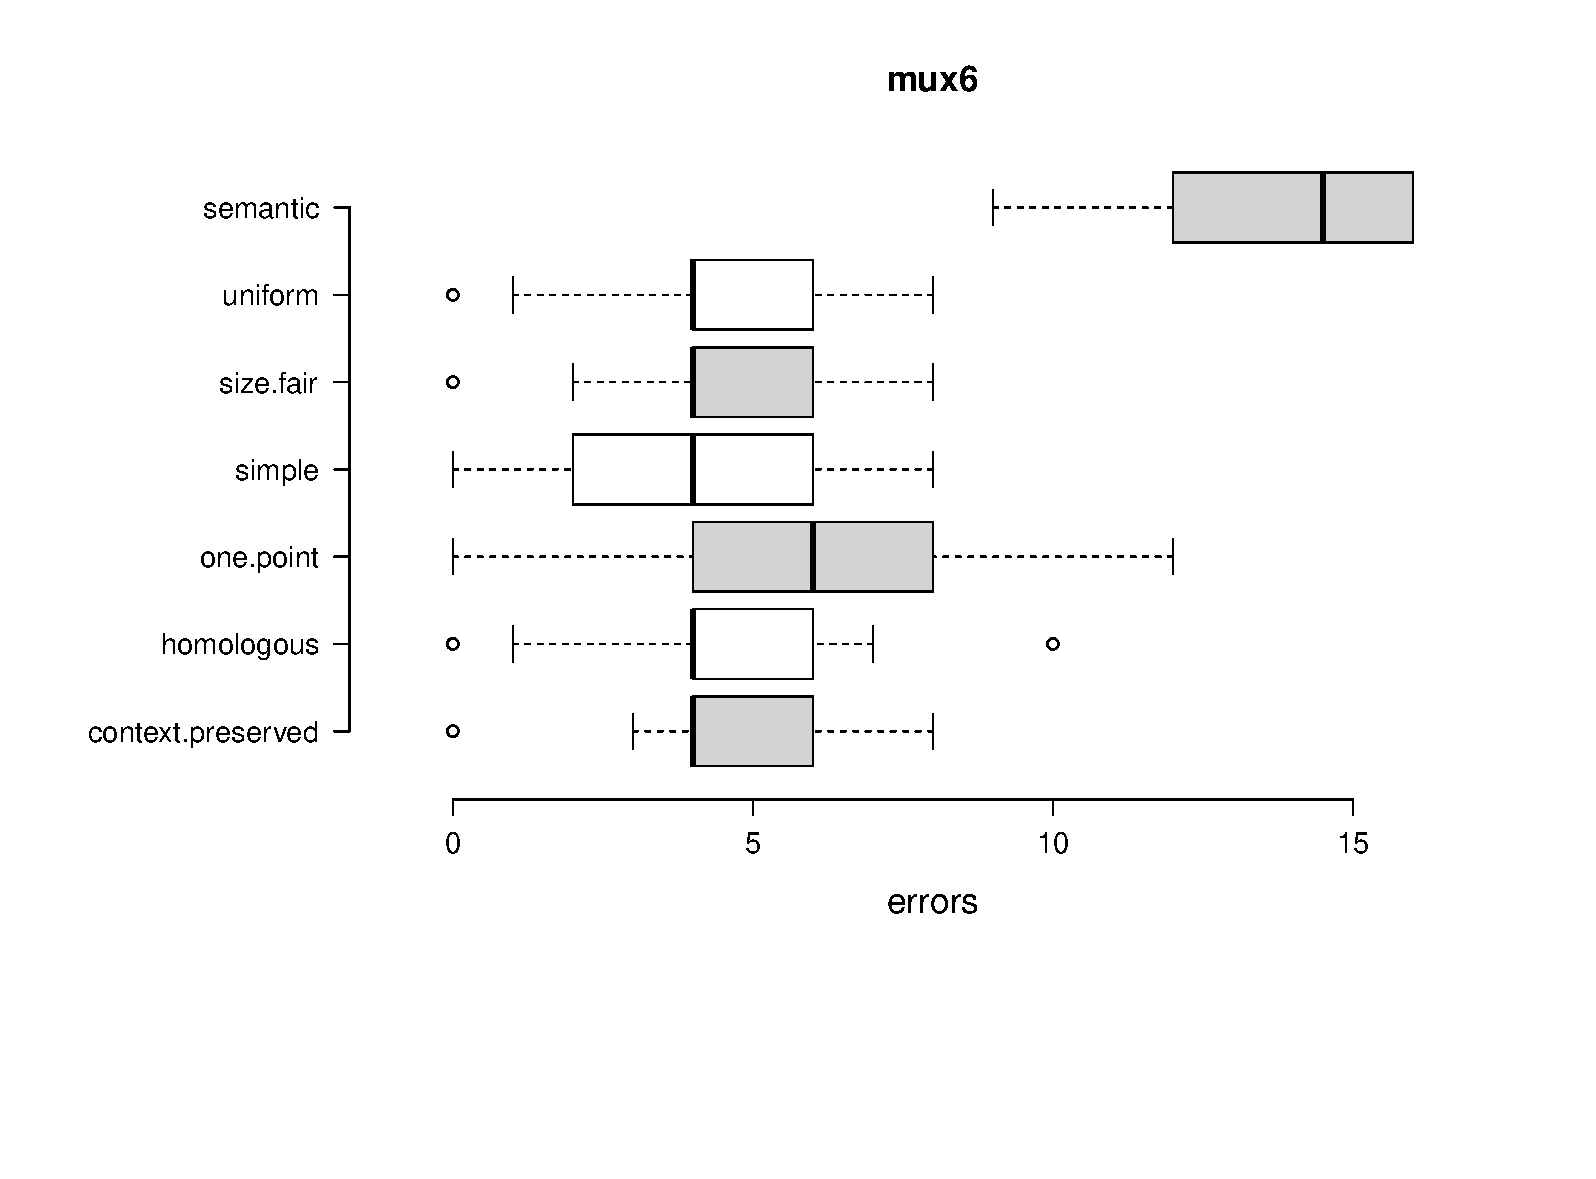
\includegraphics[trim=0cm 4cm 0cm 0cm, scale=0.6]{./slike/boxPlots/mux6.eps}
	\caption{Usporedba učinkovitosti pojedinačnih operatora križanja na problem 6 - multipleksora}
	\label{muxbox}
\end{figure}

\textbf{11 - multipleksor}

Na slici \ref{mux11box} i u tablici \ref{mux11table} prikazani su rezultati usporedbe operatora nad problemom 11 - multipleksor. Za ovaj eksperiment korišteni su konstanti parametri:
\begin{itemize}
\item{veličina populacije = 200}
\item{broj evaluacija = 8000}
\item{faktor mutacije = 0.3}
\item{nezavršni znakovi: \textit{AND, OR, NOT, IF}}
\item{završni znakovi: \textit{$a_0, a_1, a_2, d_0, d_1, d_2, d_3, d_4, d_5, d_6, d_7$}}
\end{itemize}

Iz rezultata je vidljivo kako se u ovom slučaju kao najbolje križanje pokazalo jednostavno. Jednako kao i za prethodni 6 - multipleksor problem, semantičko križanje je postiglo daleko najgore rezultate. Iz ovoga se može zaključiti kako semantičko križanje zasigurno nije odgovarajuće križanje za evoluiranje funkcije multipleksora. Ostali operatori postigli su sasvim zadovoljavajuće rezultate, s prosječnim brojem pogrešaka koje značajnije ne odstupaju od onog kod jednostavnog križanja.

\begin{table}[H]
 	\centering
  \caption{Medijani broja pogrešaka dobivene usporedbom operatora nad problemom 11 - multipleksor}
    \begin{tabular}{| l | l | l |}
    \hline
    \textbf{operator} & \textbf{medijan broj pogrešaka} & \textbf{rang}\\ \hline
    simple & 416 &1\\ \hline
    one point & 480 & 6\\ \hline
    context preserved & 456 & 3\\ \hline
    size fair & 432 & 2\\ \hline
    uniform & 470 & 4\\ \hline
    homologous & 476 & 5\\ \hline
    semantic & 736 & 7\\ \hline
    \end{tabular}
    
  
    \label{mux11table}
\end{table}

\begin{figure}[H]
	\centering
	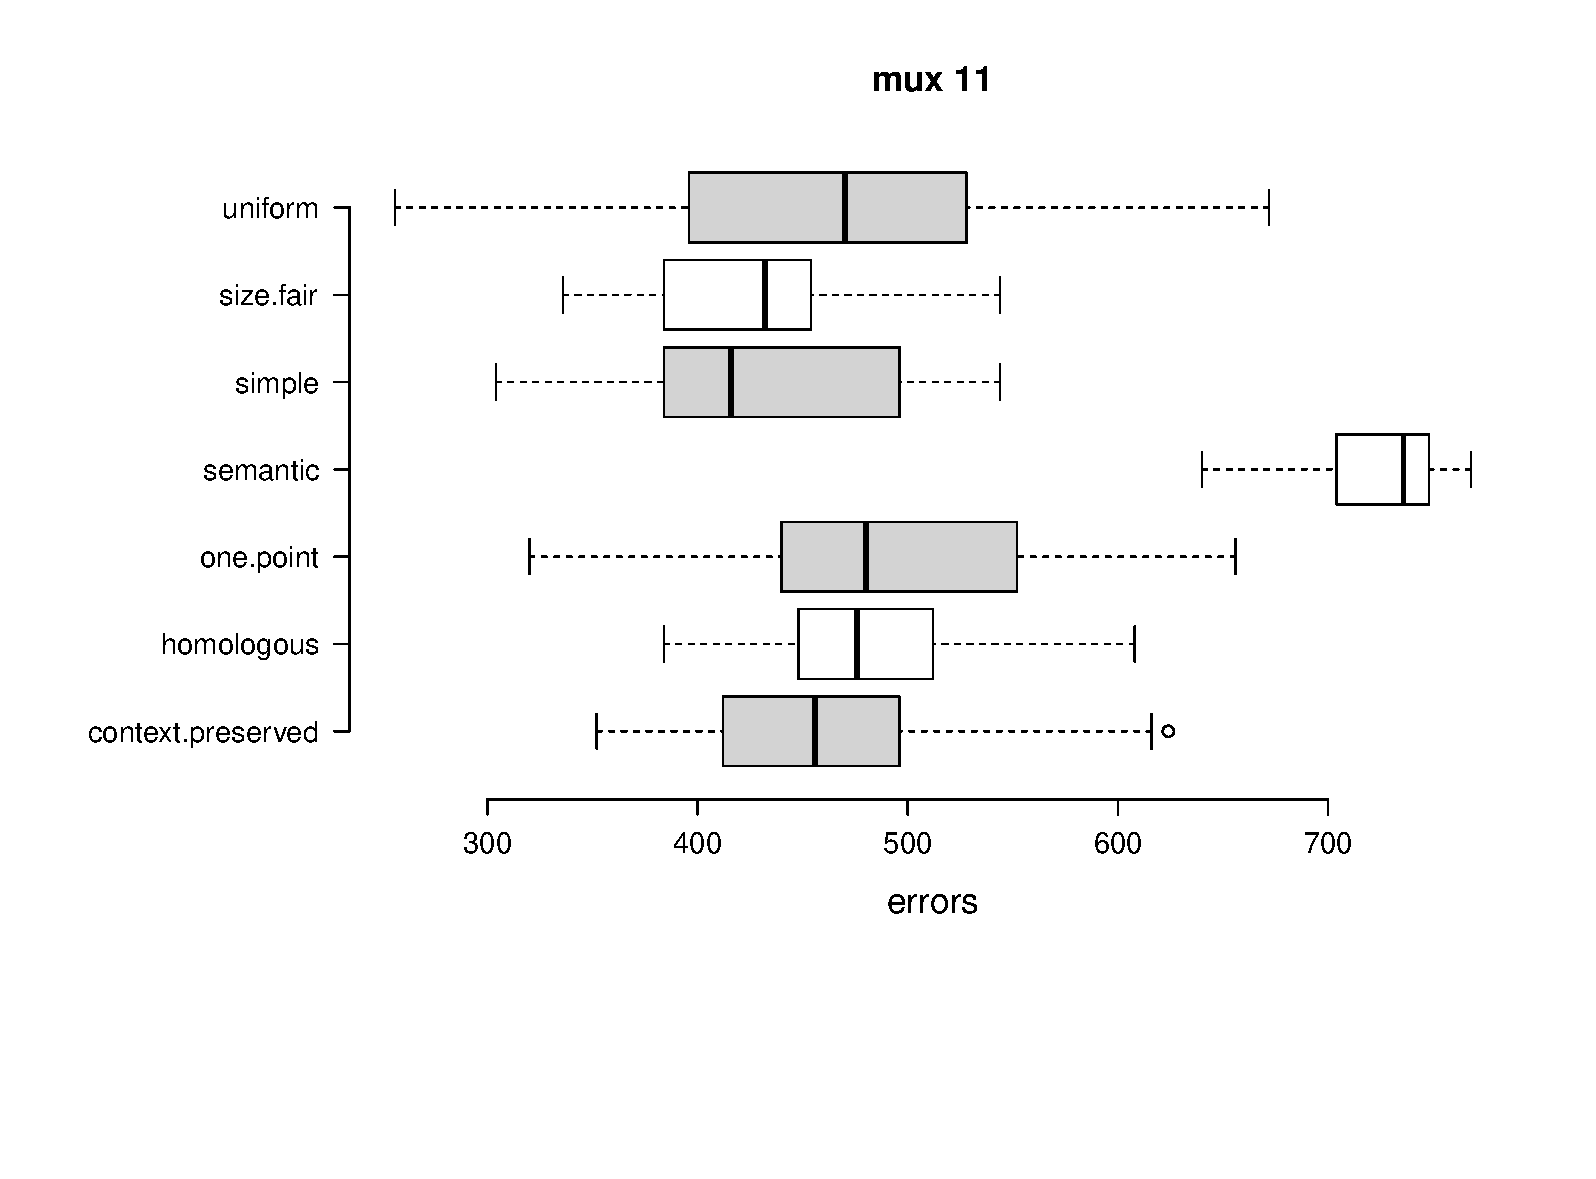
\includegraphics[trim=0cm 4cm 0cm 0cm, scale=0.6]{./slike/boxPlots/mux11.eps}
	\caption{Usporedba učinkovitosti pojedinačnih operatora križanja na problem 11 - multipleksora}
	\label{mux11box}
\end{figure}

\textbf{Evolucija kriptografski sigurnih logičkih funkcija - inačica 1}

Inačice ovog eksperimenta razlikuju se u izračunu funkcije dobrote - u ovom slučaju, funkcija dobrote u obzir uzima balans i nelinearnost evoluirane funkcije. Radi duljine izvršavanja evolucije ovakvih funkcija, za svaki operator, eksperiment je pokrenut 20 puta. Za ovaj eksperiment korišteni su konstanti parametri:
\begin{itemize}
\item{veličina populacije = 250}
\item{broj evaluacija = 3750}
\item{faktor mutacije = 0.3}
\item{nezavršni znakovi: \textit{AND OR NOT IF XOR}}
\item{završni znakovi: \textit{$v_0, v_1, v_2, v_3, v_4, v_5, v_6, v_7$}}
\end{itemize}

Na slici \ref{bool1box} i u tablici \ref{bool1table} prikazani su rezultati provedenog eksperimenta. Vidljivo je kako je najbolje rezultate postiglo semantičko križanje, odnosno njegova kombinacija s jednostavnim križanjem u omjeru 1:9.

\begin{table}[H]
 	\centering
\caption{Medijani dobrote dobivene usporedbom operatora nad problemom evolucije sigurnih logičkih funkcija inačice 1}
    \begin{tabular}{| l | l | l |}
    \hline
    \textbf{operator} & \textbf{medijan dobrote} & \textbf{rang}\\ \hline
    simple & 111.061 & 3\\ \hline
    one point & 110.0645 & 6\\ \hline
    context preserved & 111.06 & 5\\ \hline
    size fair & 111.061 & 3\\ \hline
    uniform & 109.071 & 7\\ \hline
    homologous & 111.062 & 2\\ \hline
    semantic & 113.031& 1\\ \hline
    \end{tabular}
    
    
    \label{bool1table}
\end{table}

\begin{figure}[H]
	\centering
	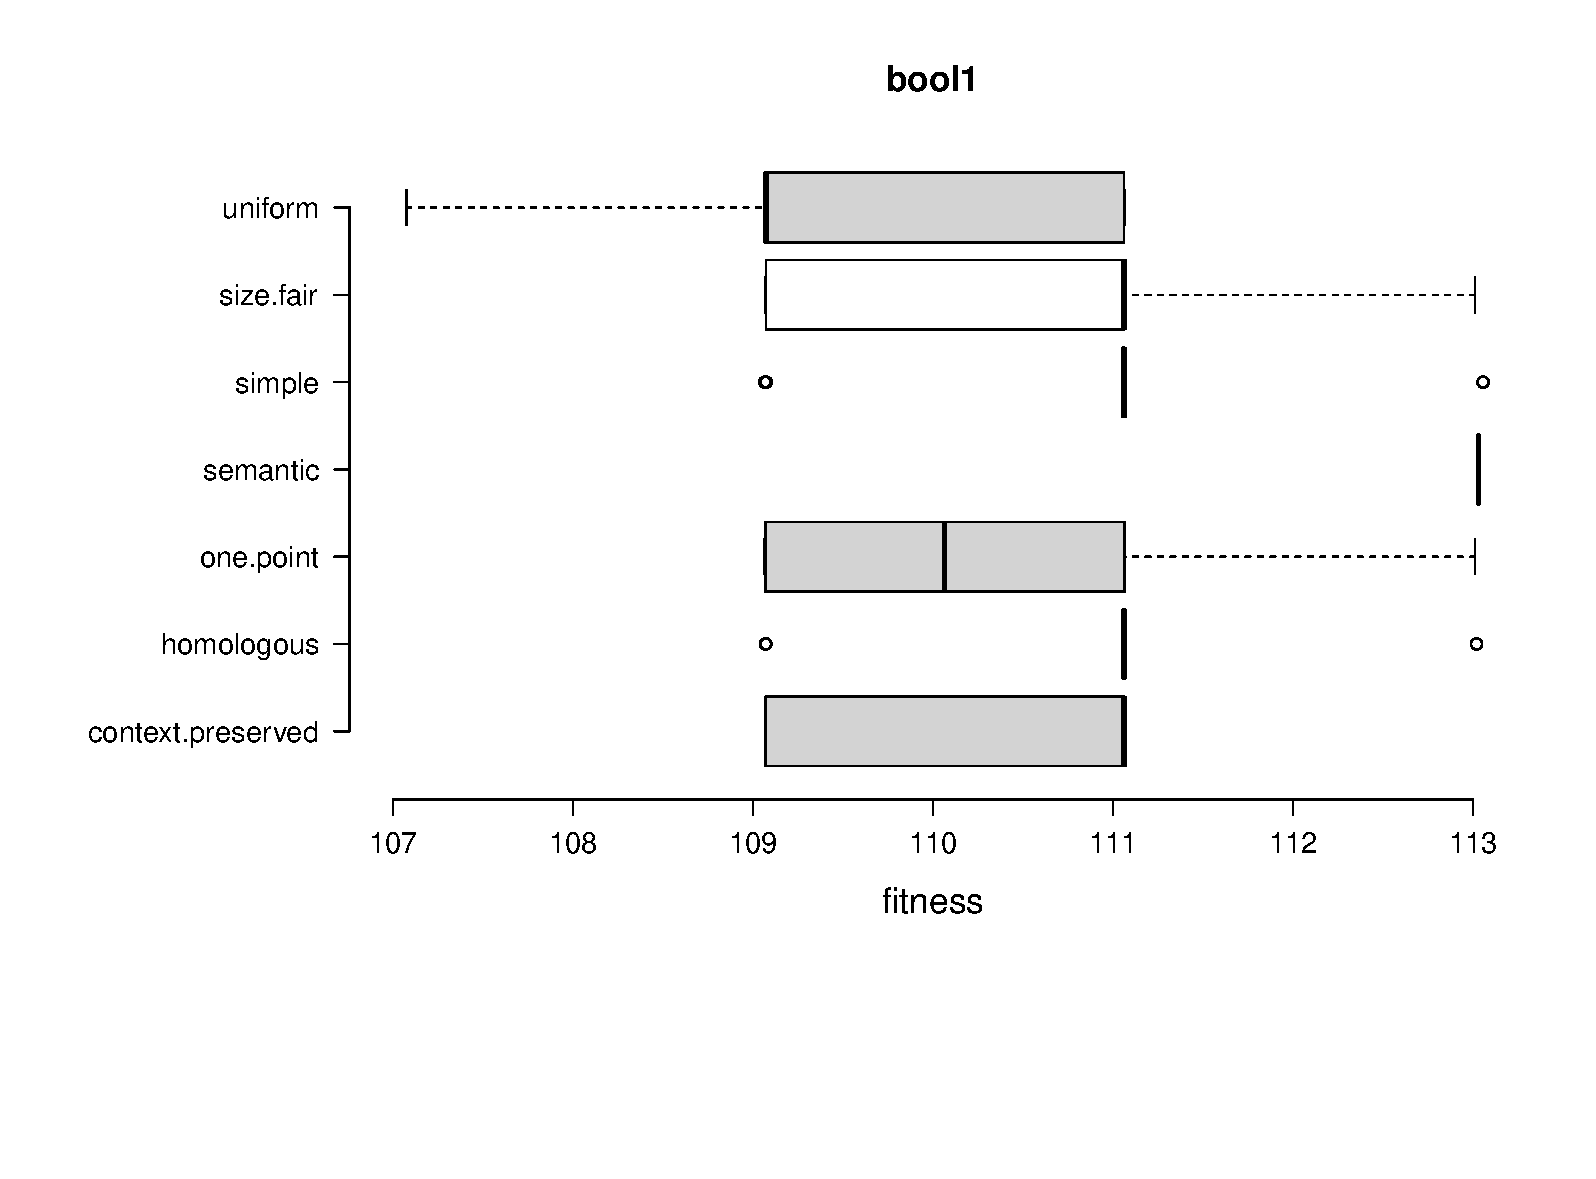
\includegraphics[trim=0cm 4cm 0cm 0cm, scale=0.5]{./slike/boxPlots/bool1.eps}
	\caption{Usporedba učinkovitosti pojedinačnih operatora križanja na problem evolucije kriptografski sigurnih logičkih funkcija inačice 1}
	\label{bool1box}
\end{figure}


\textbf{Evolucija kriptografski sigurnih logičkih funkcija - inačica 4}

U izračunu dobrote ove inačice eksperimenta, funkcija dobrote u obzir uzima transparentnost i balansiranost evoluirane funkcije. Jednako kao i za prethodnu inačicu, svaki eksperiment za ovaj problem proveden je 20 puta. Osim toga, za  ovaj eksperiment također su korišteni konstanti parametri:
\begin{itemize}
\item{veličina populacije = 250}
\item{broj evaluacija = 3750}
\item{faktor mutacije = 0.3}
\item{nezavršni znakovi: \textit{AND, OR, NOT, IF, XOR}}
\item{završni znakovi: \textit{$v_0, v_1, v_2, v_3, v_4, v_5, v_6, v_7$}}
\end{itemize}

Na slici \ref{bool4box} i u tablici \ref{bool4table} prikazani su rezultati provedenog eksperimenta. Vidljivo je kako je najbolje rezultate postiglo semantičko križanje, odnosno njegova kombinacija s jednostavnim križanjem u omjeru 1:9.

\begin{table}[H]
 	\centering
 \caption{Medijani dobrote dobivene usporedbom operatora nad problemom evolucije sigurnih logičkih funkcija inačice 4}
    \begin{tabular}{| l | l | l |}
    \hline
    \textbf{operator} & \textbf{medijan dobrote} & \textbf{rang}\\ \hline
    simple & 1.16581 & 2\\ \hline
    one point & 1.11728 & 6\\ \hline
    context preserved & 1.12635 & 5\\ \hline
    size fair & 1.14657 & 3\\ \hline
    uniform & 1.130145 & 4\\ \hline
    homologous & 1.1163 & 7\\ \hline
    semantic & 1.185785 & 1\\ \hline
    \end{tabular}
    
   
    \label{bool4table}
\end{table}


Iz prethodna dva eksperimenta može se zaključiti kako je za evoluciju kriptografski sigurnih funkcija najučinkovitije semantičko križanje u kombinaciji s jednostavnim u omjeru od 1:9.

\begin{figure}[H]
	\centering
	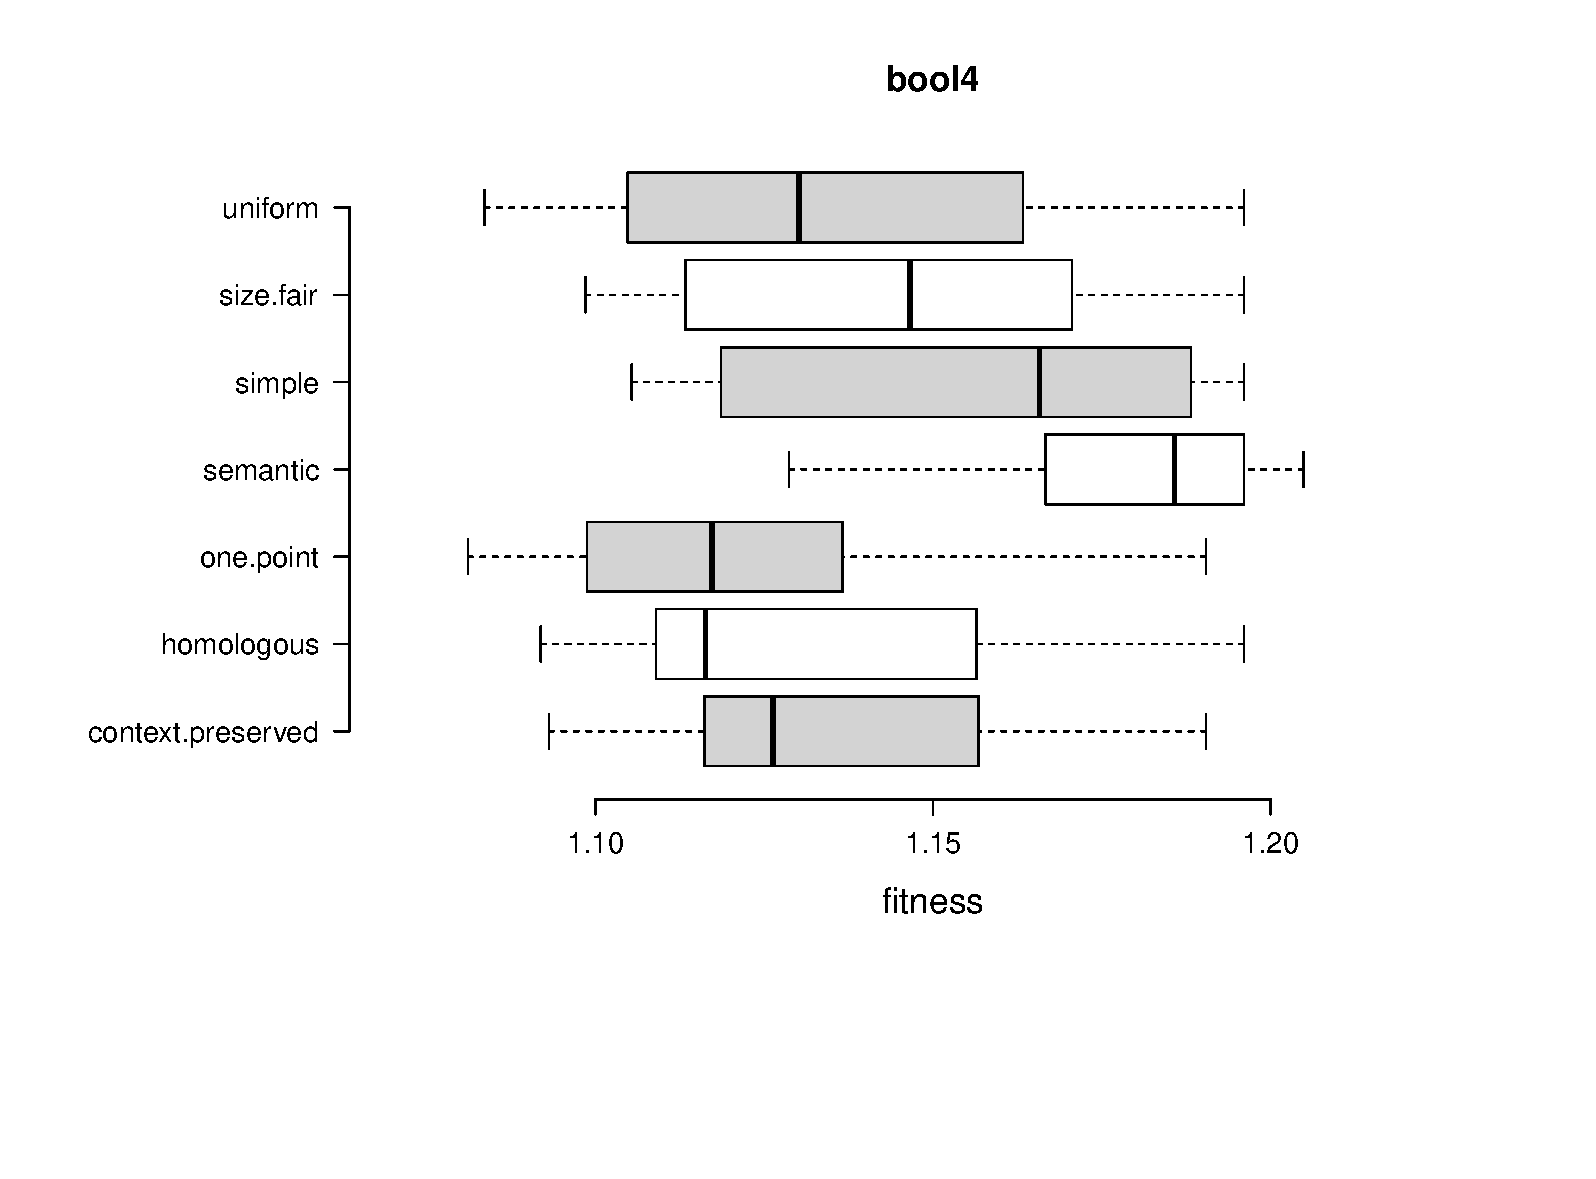
\includegraphics[trim=0cm 4cm 0cm 0cm, scale=0.6]{./slike/boxPlots/bool4.eps}
	\caption{Usporedba učinkovitosti pojedinačnih operatora križanja na problem evolucije kriptografski sigurnih logičkih funkcija inačice 4}
	\label{bool4box}
\end{figure}


\subsubsection{Simbolička regresija}

Za probleme simboličke regresije, provedeni su eksperimenti koji su međusobno usporedili jednostavno križanje, križanje s jednom točkom prekida, križanje s očuvanjem konteksta, križanje pravedno s obzirom na veličinu, uniformno, homologno, semantičko, determinističko i probabilističko križanje.

\textbf{Klasična simbolička regresija}


Na grafovima u nastavku prikazana je učinkovitost pojedinih operatora križanja na probleme klasične simboličke regresije predstavljene na početku poglavlja. U ovom slučaju, potrebno je minimizirati funkciju dobrote koja se računa kao srednja kvadratna pogreška. U svim slučajevima, probabilističko križanje pokazalo se kao daleko najlošije - dobrota jedinki dobivenih ovim križanjem redovito je odskakala od ostalih za jedan red veličine. Radi toga, na grafovima u nastavku nije uključeno to križanje iz razloga što bi pokvarilo njihovu razlučivost.

Na slici \ref{symb1box} i u tablici \ref{symb1table} prikazana je učinkovitost operatora križanja prilikom rješavanja prvog problema simboličke regresije (symb1). Za ovaj eksperiment korišteni su konstanti parametri:
\begin{itemize}
\item{veličina populacije = 400}
\item{broj generacija = 200}
\item{faktor mutacije = 0.5}
\item{nezavršni znakovi: \textit{log, +, -, *}}
\item{završni znakovi: \textit{x, 1}}
\end{itemize}

Vidljivo je kako je za ovaj problem daleko najučinkovitiji bio operator semantičkog križanja, odnosno kombinacije semantičkog i jednostavnog križanja u omjeru 1:9. 


\begin{table}[H]
 	\centering
 \caption{Medijani srednje kvadratne pogreške dobivene usporedbom operatora nad problemom simboličke regresije symb1}
    \begin{tabular}{| l | l | l |}
    \hline
    \textbf{operator} & \textbf{medijan mse-a} & \textbf{rang}\\ \hline
    simple & 0.8796885 & 3\\ \hline
    one point & 1.06746 & 6\\ \hline
    context preserved & 0.8924265 & 4\\ \hline
    size fair & 0.7988625 & 2\\ \hline
    uniform & 1.038325 & 5\\ \hline
    homologous & 1.25174 & 8\\ \hline
    deterministic & 1.120405 & 7\\ \hline
    probabilistic & 18.16455 & 9\\ \hline
    semantic & 0.1364575 & 1\\ \hline
    \end{tabular}
    
   
    \label{symb1table}
\end{table}

\begin{figure}[H]
	\centering
	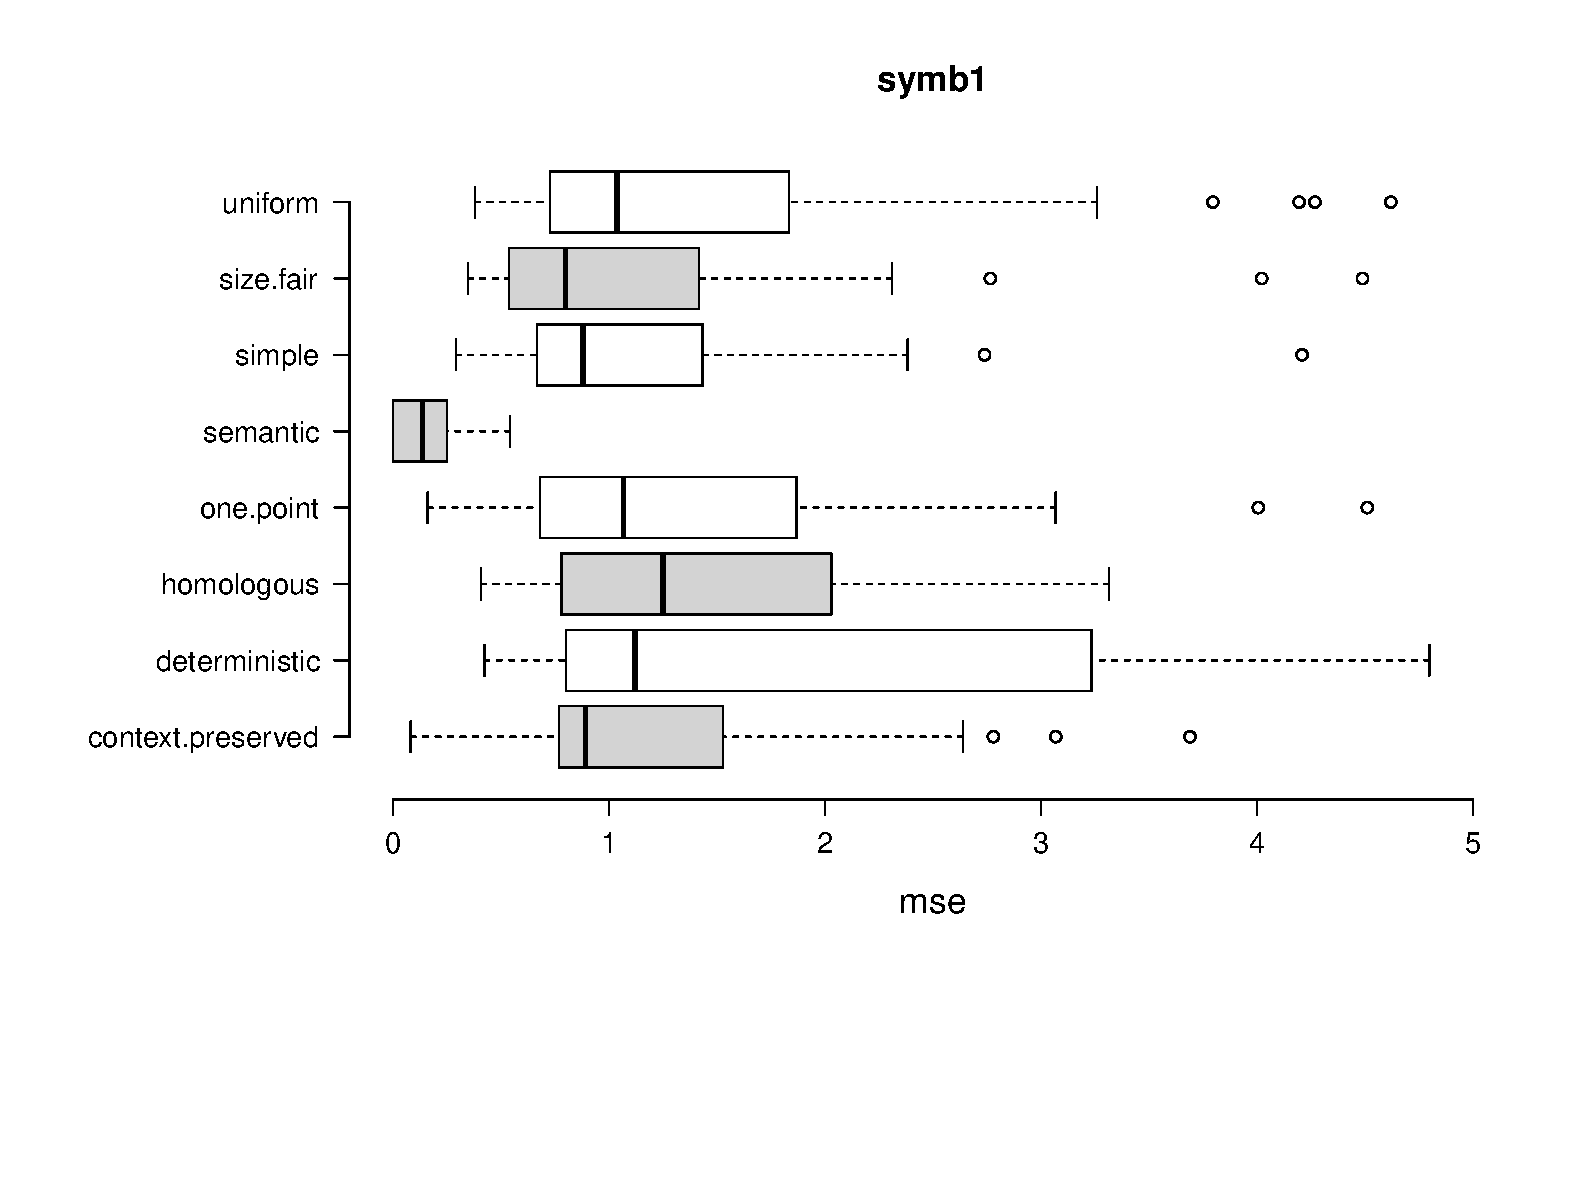
\includegraphics[trim=0cm 4cm 0cm 0cm, scale=0.6]{./slike/boxPlots/symb1.eps}
	\caption{Usporedba učinkovitosti pojedinačnih operatora križanja na problem simboličke regresije symb1}
	\label{symb1box}
\end{figure}



Na slici \ref{symb2box} prikazana je usporedba učinkovitosti operatora na problemu simboličke regresije symb2. Za ovaj eksperiment korišteni su konstanti parametri:
\begin{itemize}
\item{veličina populacije = 100}
\item{broj generacija = 50}
\item{faktor mutacije = 0.2}
\item{nezavršni znakovi: \textit{sin, *, +, -, /}}
\item{završni znakovi: \textit{x, y}}
\end{itemize} 

Na slici \ref{symb2box} i u tablici \ref{symb2table} jednostavno križanje, križanje pravedno s obzirom na veličinu i kombinacija semantičkog i jednostavnog križanja postigli su najbolje rezultate. Ostali operatori su se pokazali kao znatno lošiji prilikom rješavanja ovog problema.

\begin{table}[H]
 	\centering
 \caption{Medijani srednje kvadratne pogreške dobivene usporedbom operatora nad problemom simboličke regresije symb2}
    \begin{tabular}{| l | l | l |}
    \hline
    \textbf{operator} & \textbf{medijan mse-a}  & \textbf{rang}\\ \hline
    simple & 0 & 1\\ \hline
    one point & 8.07678 & 8\\ \hline
    context preserved & 4.02037 & 5\\ \hline
    size fair & 0 & 1\\ \hline
    uniform & 4.6308 & 7\\ \hline
    homologous & 4.02037 & 5\\ \hline
    deterministic &2.66101 & 4\\ \hline
    probabilistic & 12.3481 & 9\\ \hline
    semantic & 0 & 1\\ \hline
    \end{tabular}
    
   
    \label{symb2table}
\end{table}

\begin{figure}[H]
	\centering
	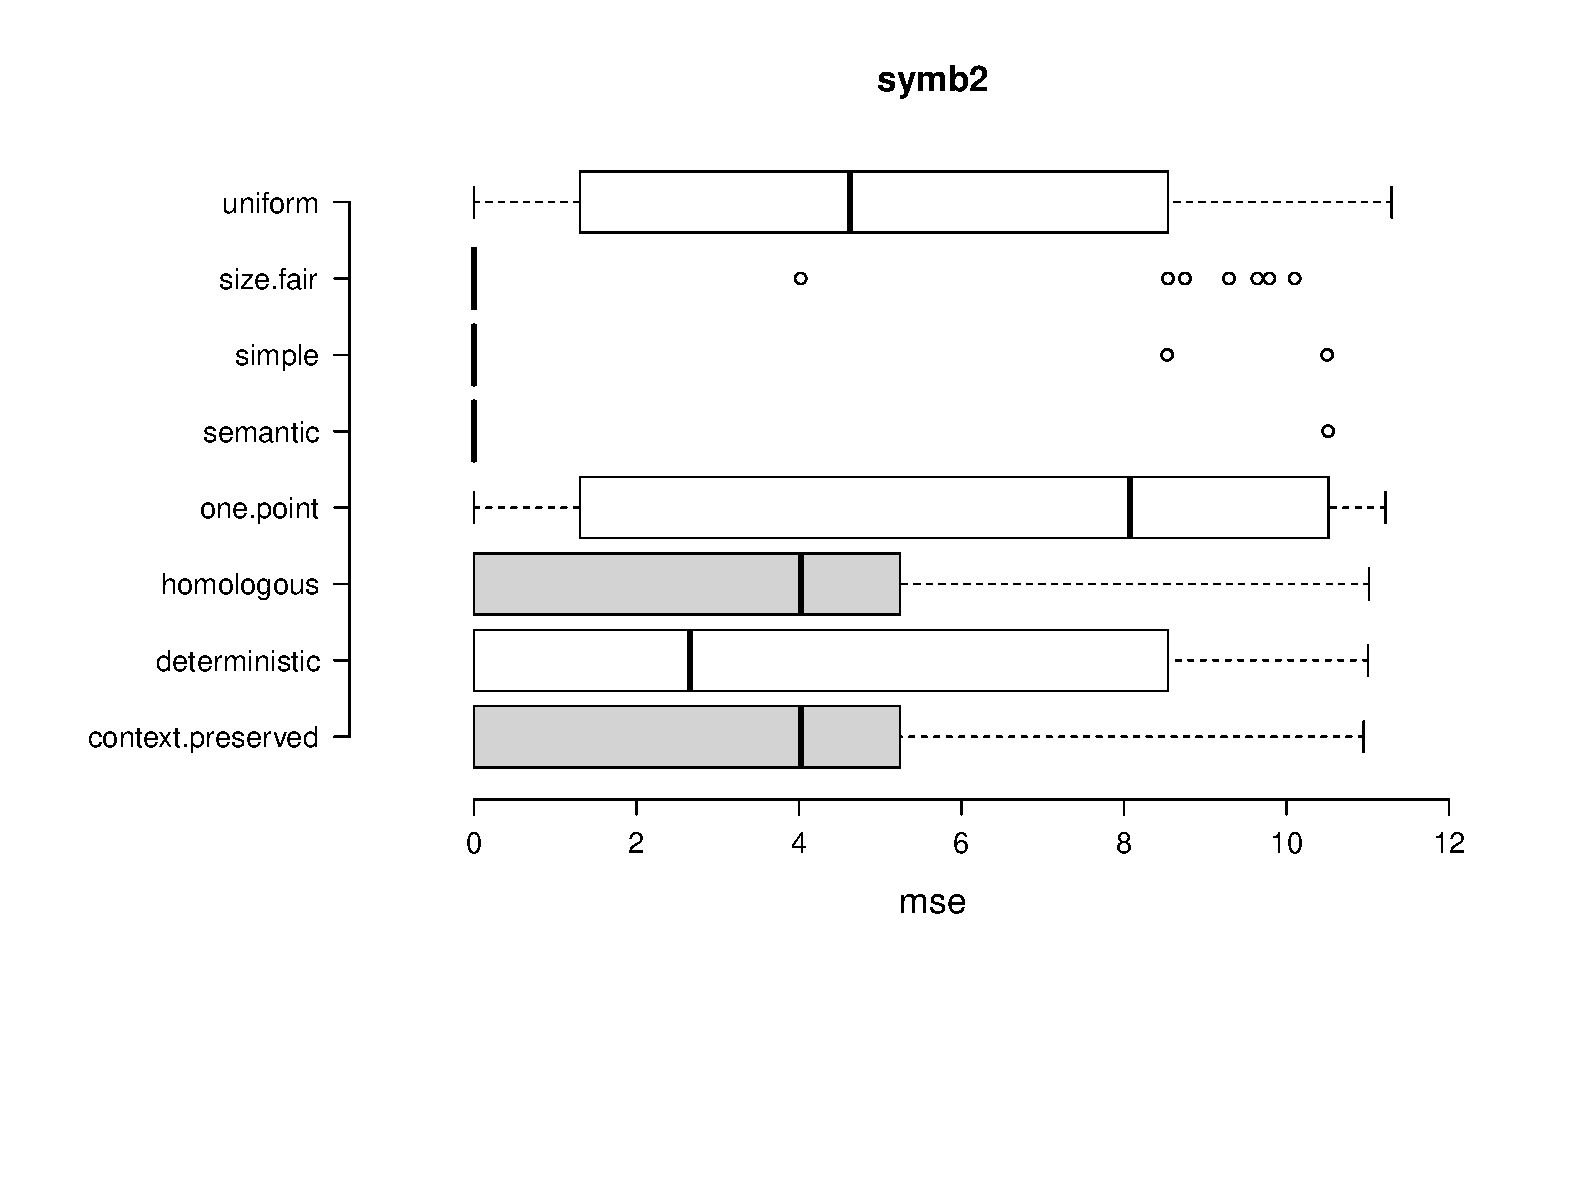
\includegraphics[trim=0cm 4cm 0cm 0cm, scale=0.6]{./slike/boxPlots/symb2.eps}
	\caption{Usporedba učinkovitosti pojedinačnih operatora križanja na problem simboličke regresije symb2}
	\label{symb2box}
\end{figure}

\begin{table}[H]
 	\centering

    \caption{Medijani srednje kvadratne pogreške dobivene usporedbom operatora nad problemom simboličke regresije symb3}
    \begin{tabular}{| l | l | l |}
    \hline
    \textbf{operator} & \textbf{medijan mse-a} & \textbf{rang}\\ \hline
    simple & $7.77 \cdot 10^{-16}$ & 1\\ \hline
    one point & $7.77 \cdot 10^{-16}$ & 1\\ \hline
    context preserved &$7.77 \cdot 10^{-16}$& 1 \\ \hline
    size fair & $7.77 \cdot 10^{-16}$ & 1\\ \hline
    uniform & $7.77 \cdot 10^{-16}$ & 1\\ \hline
    homologous & $7.77 \cdot 10^{-16}$ & 1\\ \hline
    deterministic & $7.77 \cdot 10^{-16}$ & 1\\ \hline
    probabilistic & $7.77 \cdot 10^{-16}$ & 1\\ \hline
    semantic & $1.39 \cdot 10^{-15}$ & 9\\ \hline
    \end{tabular}
    
    \label{symb3table}
\end{table}

\begin{figure}[H]
	\centering
	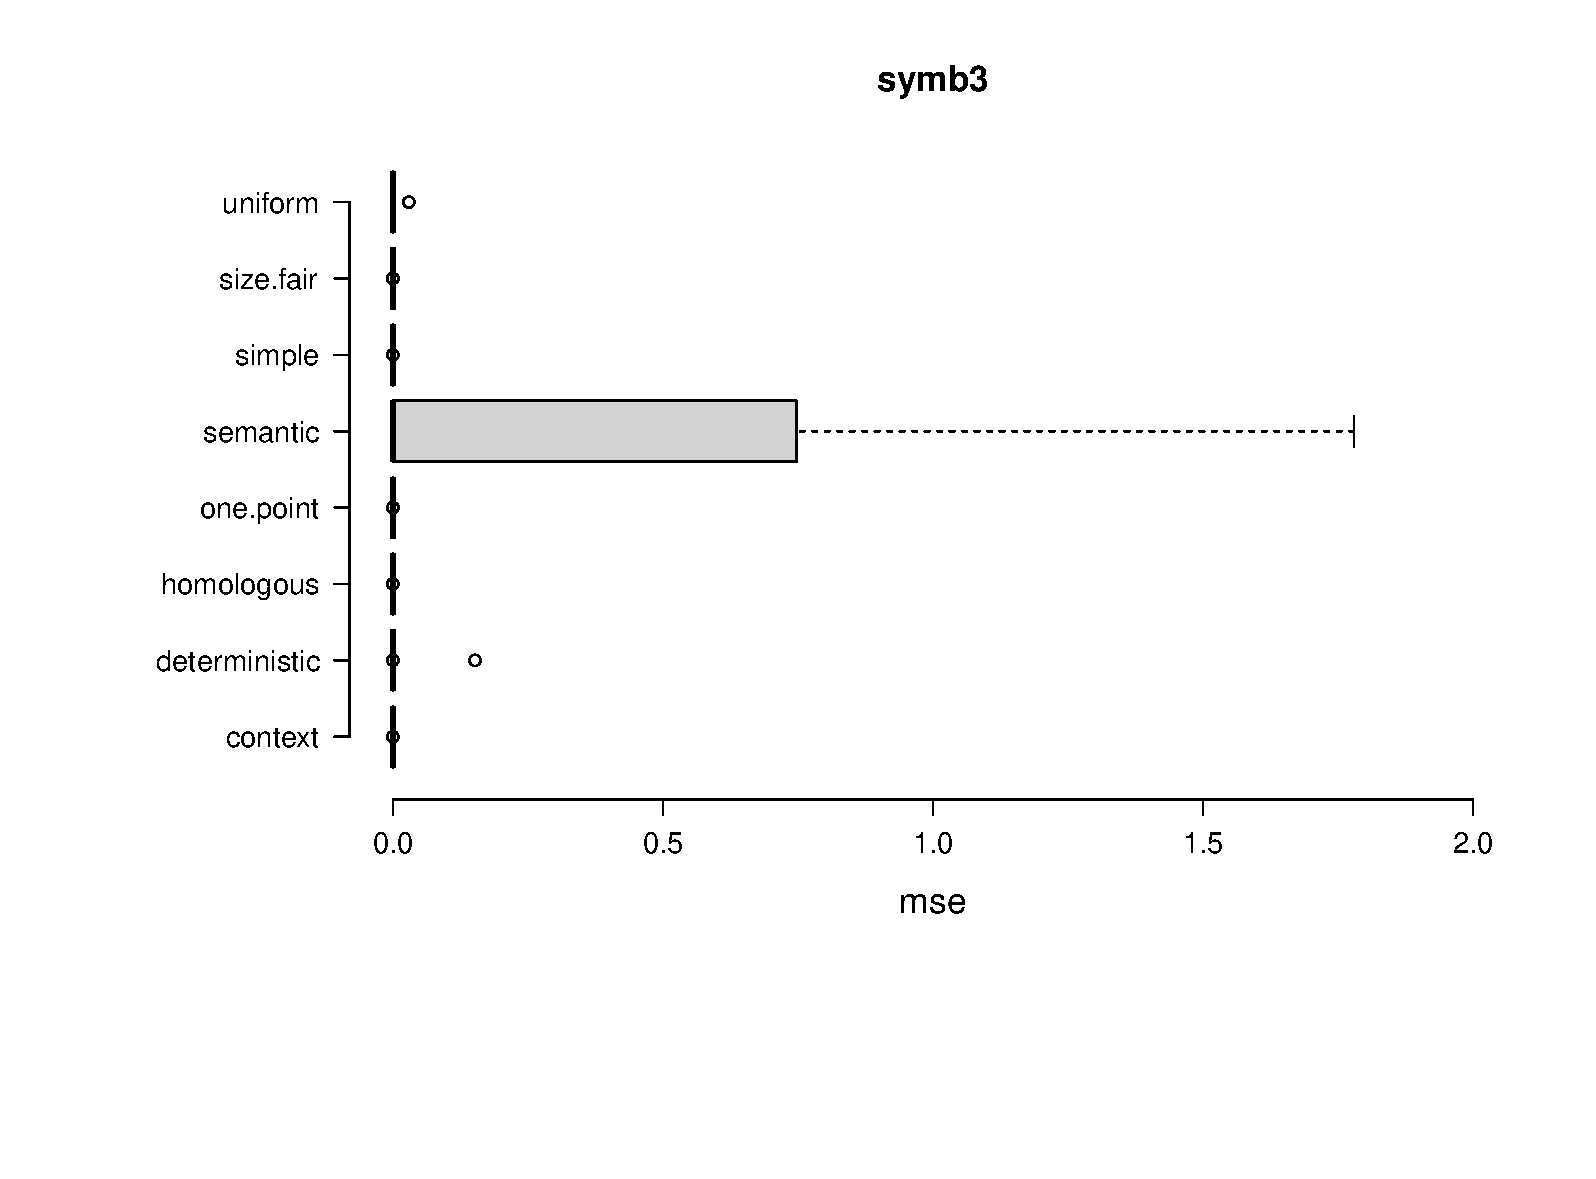
\includegraphics[trim=0cm 4cm 0cm 0cm, scale=0.6]{./slike/boxPlots/symb3.eps}
	\caption{Usporedba učinkovitosti pojedinačnih operatora križanja na problem simboličke regresije symb3}
	\label{symb3box}
\end{figure}

Na slici \ref{symb3box} i u tablici \ref{symb3table} prikazana je usporedba učinkovitosti operatora na problemu simboličke regresije symb3. Za ovaj eksperiment korišteni su konstanti parametri:
\begin{itemize}
\item{veličina populacije = 400}
\item{broj generacija = 50}
\item{faktor mutacije = 0.3}
\item{nezavršni znakovi: \textit{sin, cos, *, +, -, /}}
\item{završni znakovi: \textit{x, y, 2}}
\end{itemize} 

Vidljivo je kako je ovaj problem ispao prilično lagan za sve operatore - jedini operator koji je bio nešto neučinkovitiji bio je semantički operator križanja (odnosno, njegova kombinacija s jednostavnim križanjem u omjeru 1:9) koji u nekoliko pokretanja nije uspio pronaći točno rješenje. Također, u ovom slučaju zanimljivo je primijetiti kako je probabilističko križanje postiglo medijan dobrote vrlo blizu nuli - što uvelike odskače od dosadašnjih rezultata ovog operatora koji su bili iznenađujuće loši. Moguć razlog ovom rezultatu jest činjenica da se ovaj problem pokazao prilično jednostavan i za sve ostale operatore.
\\

Na slici \ref{symb4box} i u tablici \ref{symb4table} prikazana je usporedba učinkovitosti operatora na problemu simboličke regresije symb4. Za ovaj eksperiment korišteni su konstanti parametri:
\begin{itemize}
\item{veličina populacije = 500}
\item{broj generacija = 200}
\item{faktor mutacije = 0.2}
\item{nezavršni znakovi: \textit{sin, *, +, -, /}}
\item{završni znakovi: \textit{x, y, 1}}
\end{itemize} 

Iz rezultata je vidljivo kako su jednostavni i semantički operator križanja postigli izvrsne rezultate, dok su ostali operatori nešto lošije riješili problem. Razlog efikasnosti kombinacije semantičkog s jednostavnim križanjem u omjeru 1:9 vjerojatno leži u tome da se semantičko križanje vrši u svega 10\% slučajeva križanja.


\begin{table}[H]
 	\centering
\caption{Medijani srednje kvadratne pogreške dobivene usporedbom operatora nad problemom simboličke regresije symb4}
    \begin{tabular}{| l | l | l |}
    \hline
    \textbf{operator} & \textbf{medijan mse-a} & \textbf{rang}\\ \hline
    simple & 0 & 1\\ \hline
    one point & 6.284285 & 5\\ \hline
    context preserved & 4.151965 & 3\\ \hline
    size fair & 5.709685 & 4\\ \hline
    uniform & 9.716085 & 8\\ \hline
    homologous & 7.300545 & 7\\ \hline
    deterministic & 7.22765 & 6\\ \hline
    probabilistic & 12.7275 & 9\\ \hline
    semantic & 0 & 1\\ \hline
    \end{tabular}
    
    
    \label{symb4table}
\end{table}

\begin{figure}[H]
	\centering
	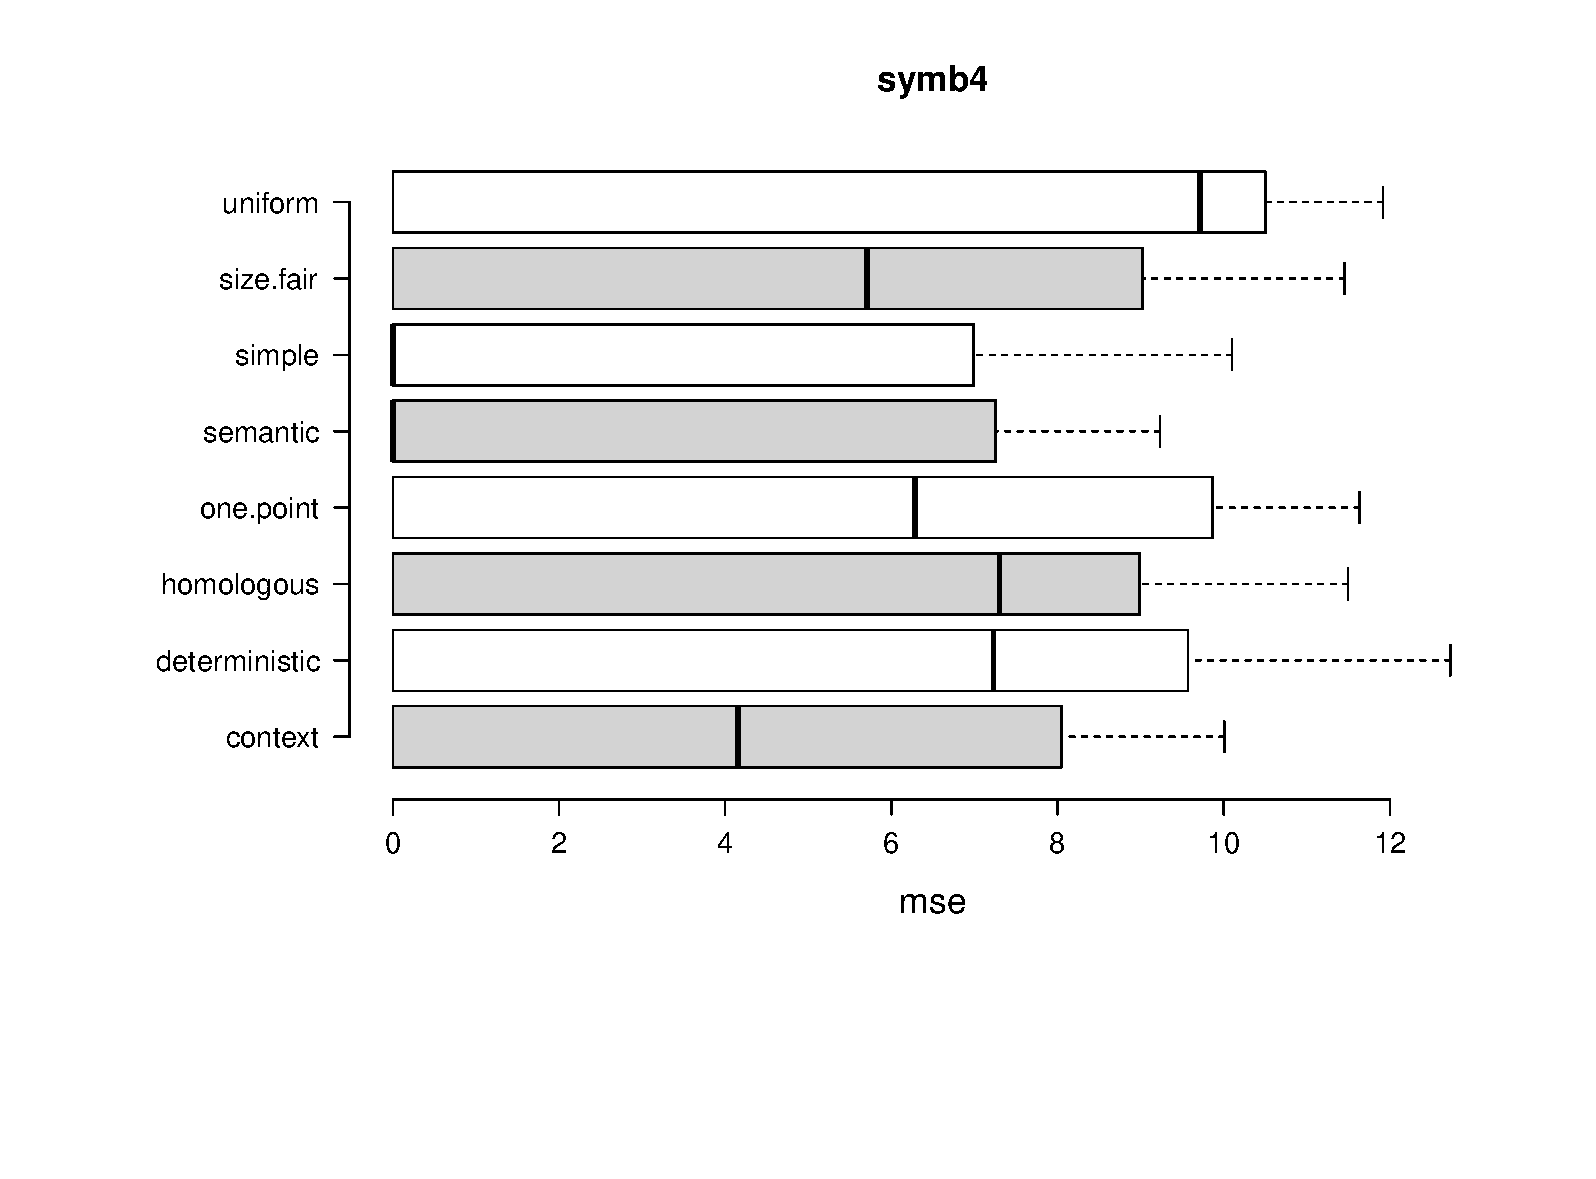
\includegraphics[trim=0cm 4cm 0cm 0cm, scale=0.6]{./slike/boxPlots/symb4.eps}
	\caption{Usporedba učinkovitosti pojedinačnih operatora križanja na problem simboličke regresije symb4}
	\label{symb4box}
\end{figure}


\begin{table}[H]
 	\centering
 \caption{Medijani srednje kvadratne pogreške dobivene usporedbom operatora nad problemom simboličke regresije symb5}
 
    \begin{tabular}{| l | l | l |}
    \hline
    \textbf{operator} & \textbf{medijan mse-a} & \textbf{rang}\\ \hline
    simple & 0 & 1\\ \hline
    one point & 0 & 1\\ \hline
    context preserved & $2.22 \cdot 10^{-16}$& 8\\ \hline
    size fair & 0 & 1\\ \hline
    uniform & 0 & 1\\ \hline
    homologous & 0 & 1\\ \hline
    deterministic & 0 & 1\\ \hline
    probabilistic & 7.45469 & 9\\ \hline
    semantic & 0 & 1\\ \hline
    \end{tabular}
    
   
    \label{symb5table}
\end{table}

\begin{figure}[H]
	\centering
	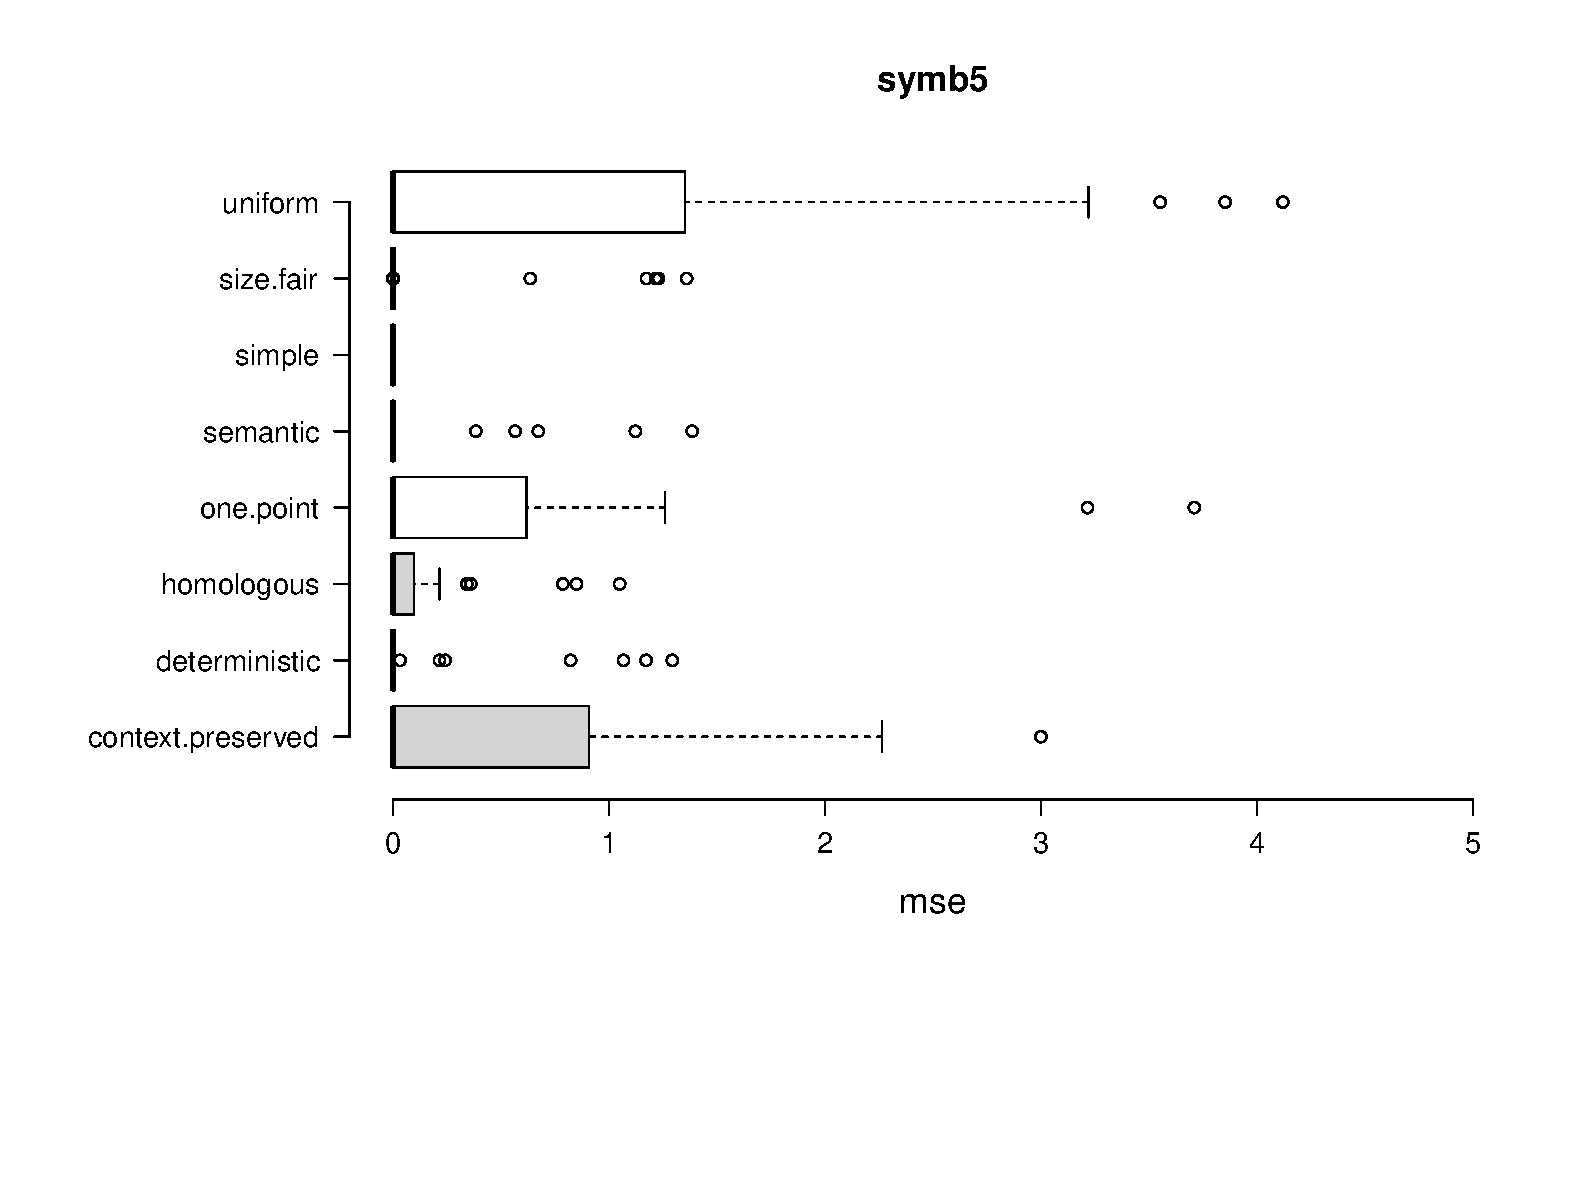
\includegraphics[trim=0cm 4cm 0cm 0cm, scale=0.6]{./slike/boxPlots/symb5.eps}
	\caption{Usporedba učinkovitosti pojedinačnih operatora križanja na problem simboličke regresije symb5}
	\label{symb5box}
\end{figure}


Na slici \ref{symb5box} i u tablici \ref{symb5table} prikazana je usporedba učinkovitosti operatora na problemu simboličke regresije symb5. Za ovaj eksperiment korišteni su konstanti parametri:
\begin{itemize}
\item{veličina populacije = 500}
\item{broj generacija = 200}
\item{faktor mutacije = 0.4}
\item{nezavršni znakovi: \textit{+, -, *, /}}
\item{završni znakovi: \textit{x, y, 2, 8}}
\end{itemize} 

U prosjeku, rješenje ovog problema uspješno su pronašli svi operatori. Po običaju, probabilističko križanje dalo je dosta lošije rješenje od ostalih, dok je križanje s očuvanjem konteksta pronašlo prilično dobro rješenje. 

\begin{table}[H]
 	\centering
    \caption{Medijani srednje kvadratne pogreške pogrešaka dobivene usporedbom operatora nad problemom simboličke regresije symb6}
    
    \begin{tabular}{| l | l | l |}
    \hline
    \textbf{operator} & \textbf{medijan mse-a} & \textbf{rang}\\ \hline
    simple & 20.1 & 4\\ \hline
    one point & 43.6 & 7\\ \hline
    context preserved & 52.9 & 8\\ \hline
    size fair & 2.13 & 2\\ \hline
    uniform & 25 & 5\\ \hline
    homologous & 32.9 & 6\\ \hline
    deterministic & 16.7 & 3\\ \hline
    probabilistic & 1080 & 9\\ \hline
    semantic & $1.18 \cdot 10^{-13}$ & 1\\ \hline
    \end{tabular}
    

    \label{symb6table}
\end{table}

\begin{figure}[H]
	\centering
	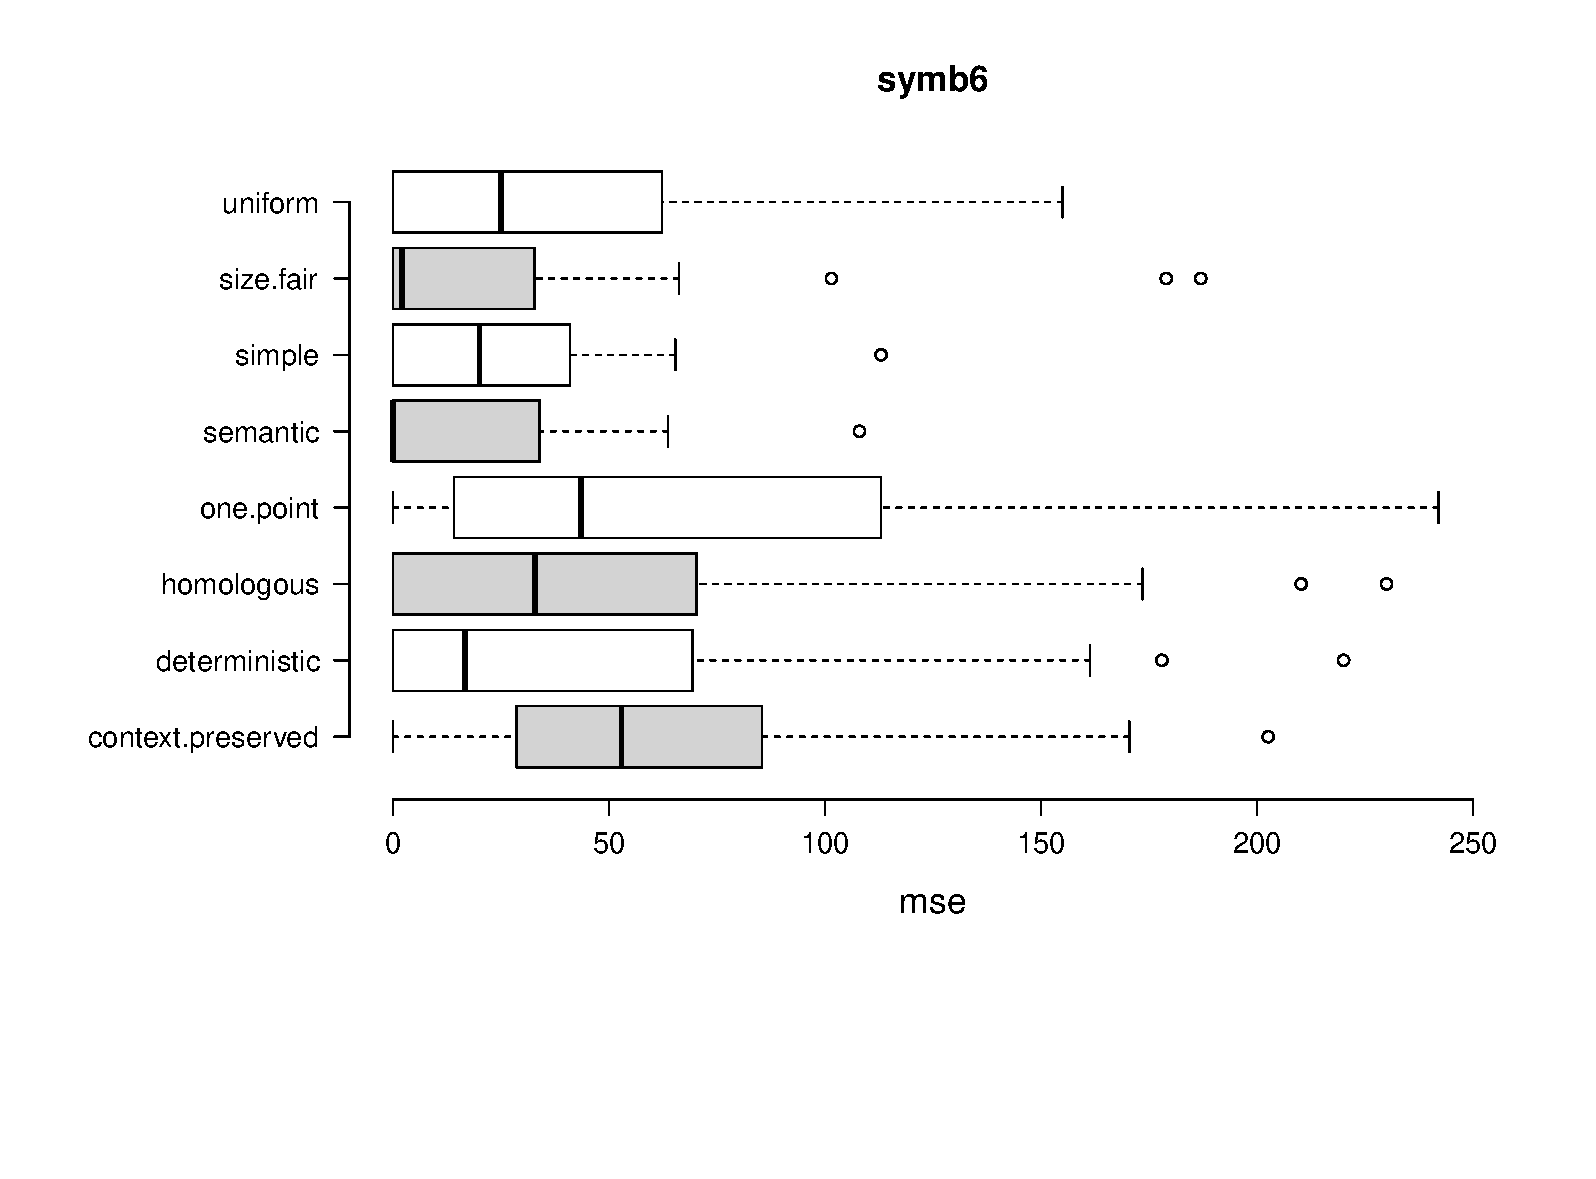
\includegraphics[trim=0cm 4cm 0cm 0cm, scale=0.5]{./slike/boxPlots/symb6.eps}
	\caption{Usporedba učinkovitosti pojedinačnih operatora križanja na problem simboličke regresije symb6}
	\label{symb6box}
\end{figure}


Na slici \ref{symb6box} i u tablici \ref{symb6table} prikazana je usporedba učinkovitosti operatora na problemu simboličke regresije symb6. Za ovaj eksperiment korišteni su konstanti parametri:
\begin{itemize}
\item{veličina populacije = 300}
\item{broj generacija = 200}
\item{faktor mutacije = 0.4}
\item{nezavršni znakovi: \textit{ +, -, *, /}}
\item{završni znakovi: \textit{x, y, 2, 5}}
\end{itemize} 

Za ovaj problem, najbolje se pokazalo semantičko križanje u kombinaciji s jednostavnim križanjem, koje je u prosjeku uvijek našlo točno rješenje.


U svim prethodno prikazanim rezultatima, najčešće se kao najučinkovitiji operator pokazao jednostavni operator križanja. Za njim slijedi kombinacija semantičkog križanja s jednostavnim križanjem, koje je u nekim slučajevima znala pronaći i bolje rješenje nego čisto jednostavno križanje. Iako bi se moglo zaključiti kako je ova kombinacija operatora učinkovita iz razloga što će u većini slučajeva upotrijebiti jednostavno križanje (koje se pokazalo kao najbolje križanje za rješavanje problema simboličke regresije) u jednom slučaju (konkretno, symb6) bilo je bolje od čistog jednostavnog križanja. To dokazuje kako je semantička komponenta te kombinacije nezanemariva i korisna.



\textbf{Evolucija funkcije prioriteta za uporabu unutar pravila raspoređivanja}

Na slici \ref{iprojektBox} u tablici \ref{iprojekttable} prikazani su rezultati usporedbe operatora na pronalaženje funkcije prioriteta za uporabu unutar pravila raspoređivanja. Za ovaj eksperiment korišteni su konstanti parametri:
\begin{itemize}
\item{veličina populacije = 500}
\item{broj generacija = 30}
\item{faktor mutacije = 0.3}
\item{nezavršni znakovi: \textit{+, -, *, /, pos}}
\item{završni znakovi: \textit{pt, dd, w, SL, pmin, pavg, PAT, MR, age}}
\end{itemize} 

\begin{table}[H]
 	\centering

    \caption{Medijani dobrote dobivene usporedbom operatora nad problemom pronalaska funkcije prioriteta za uporabu unutar pravila raspoređivanja}
    \begin{tabular}{| l | l | l |}
    \hline
    \textbf{operator} & \textbf{medijan dobrote} & \textbf{rang}\\ \hline
    simple & 16.2982 & 6\\ \hline
    one point & 16.2566 & 7\\ \hline
    context preserved & 16.1039 & 1\\ \hline
    size fair & 16.16284 & 4\\ \hline
    uniform & 16.2794 & 5\\ \hline
    homologous & 16.1527 & 3\\ \hline
    deterministic & 16.4313 & 8\\ \hline
    probabilistic & 21.30655 & 9\\ \hline
    semantic & 16.13225 & 2\\ \hline
    \end{tabular}
    
    \label{iprojekttable}
\end{table}

\begin{figure}[H]
	\centering
	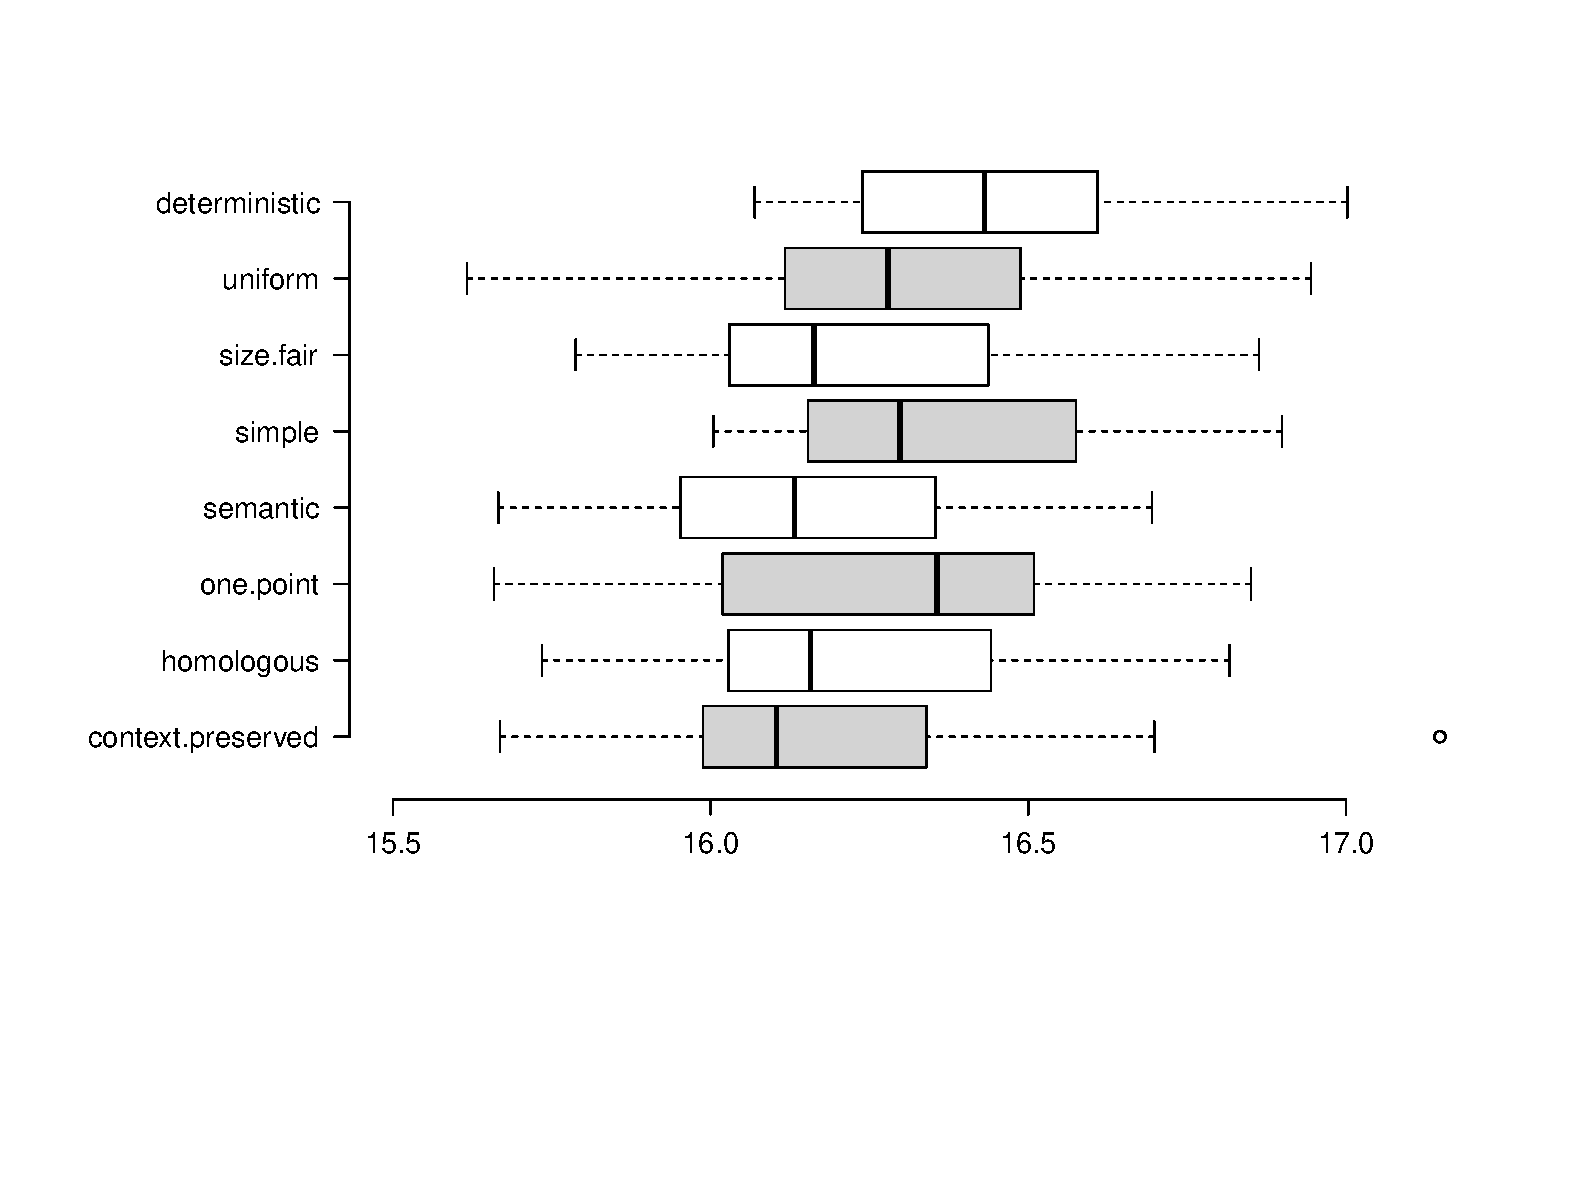
\includegraphics[trim=0cm 4cm 0cm 1cm, scale=0.6]{./slike/boxPlots/iprojekt.eps}
	\caption{Usporedba učinkovitosti pojedinačnih operatora križanja nad problemom pronalaska funkcije prioriteta za uporabu unutar pravila raspoređivanja}
	\label{iprojektBox}
\end{figure}

Iz rezultata je vidljivo kako se kao najbolji operator pokazalo križanje s očuvanje konteksta. Isto kao i za prethodne slučajeve, probabilističko križanje postiglo je znatno lošije rezultate od ostalih operatora. Zanimljivo je primijetiti značajno lošiji rang jednostavnog križanja u odnosu na prethodne rezultate.

\subsubsection{Programi}

Za programe, provedeni su eksperimenti koji su međusobno usporedili jednostavno križanje, križanje s jednom točkom prekida, križanje s očuvanjem konteksta, križanje pravedno s obzirom na veličinu, uniformno, homologno i semantičko križanje.

\textbf{Problem umjetnog mrava}

Na slici \ref{antbox} i u tablici \ref{anttable} prikazana je usporedba učinkovitosti operatora križanja na rješavanje problema umjetnoga mrava. Prikazane vrijednosti su vrijednosti na skupu za učenje, a konstantni parametri korišteni za ovaj eksperiment su:
\begin{itemize}
\item{veličina populacije = 400}
\item{broj generacija = 100}
\item{faktor mutacije = 0.4}
\item{nezavršni znakovi: \textit{Prog2, Prog3, IfFoodAhead}}
\item{završni znakovi: \textit{left, right, move}}
\end{itemize} 

Budući da je cilj algoritma maksimizirati funkciju dobrote (koja se računa kao količina pojedene hrane unutar okoline za učenje), na grafu \ref{antbox} vidljivo je kako je najučinkovitiji operator za tu zadaću jednostavno križanje. Odmah nakon njega dolazi kombinacija semantičkog i jednostavnog križanja u omjeru 1:9 te križanje pravedno s obzirom na veličinu. Križanje s jednom točkom prekida pokazalo se kao najgore u ovom slučaju.

\begin{table}[H]
 	\centering
    \caption{Medijani količine pojedene hrane za problem umjetnog mrava}
    \begin{tabular}{| l | l | l |}
    \hline
    \textbf{operator} & \textbf{medijan količine pojedene hrane} & \textbf{rang}\\ \hline
    simple & 68.5 & 1\\ \hline
    one point & 55 & 7\\ \hline
    context preserved & 56.5 & 6\\ \hline
    size fair & 62.5 & 3\\ \hline
    uniform & 60 & 5\\ \hline
    homologous & 60.5 & 4\\ \hline
    semantic & 65 & 2\\ \hline
    \end{tabular}
    

    \label{anttable}
\end{table}

\begin{figure}[H]
	\centering
	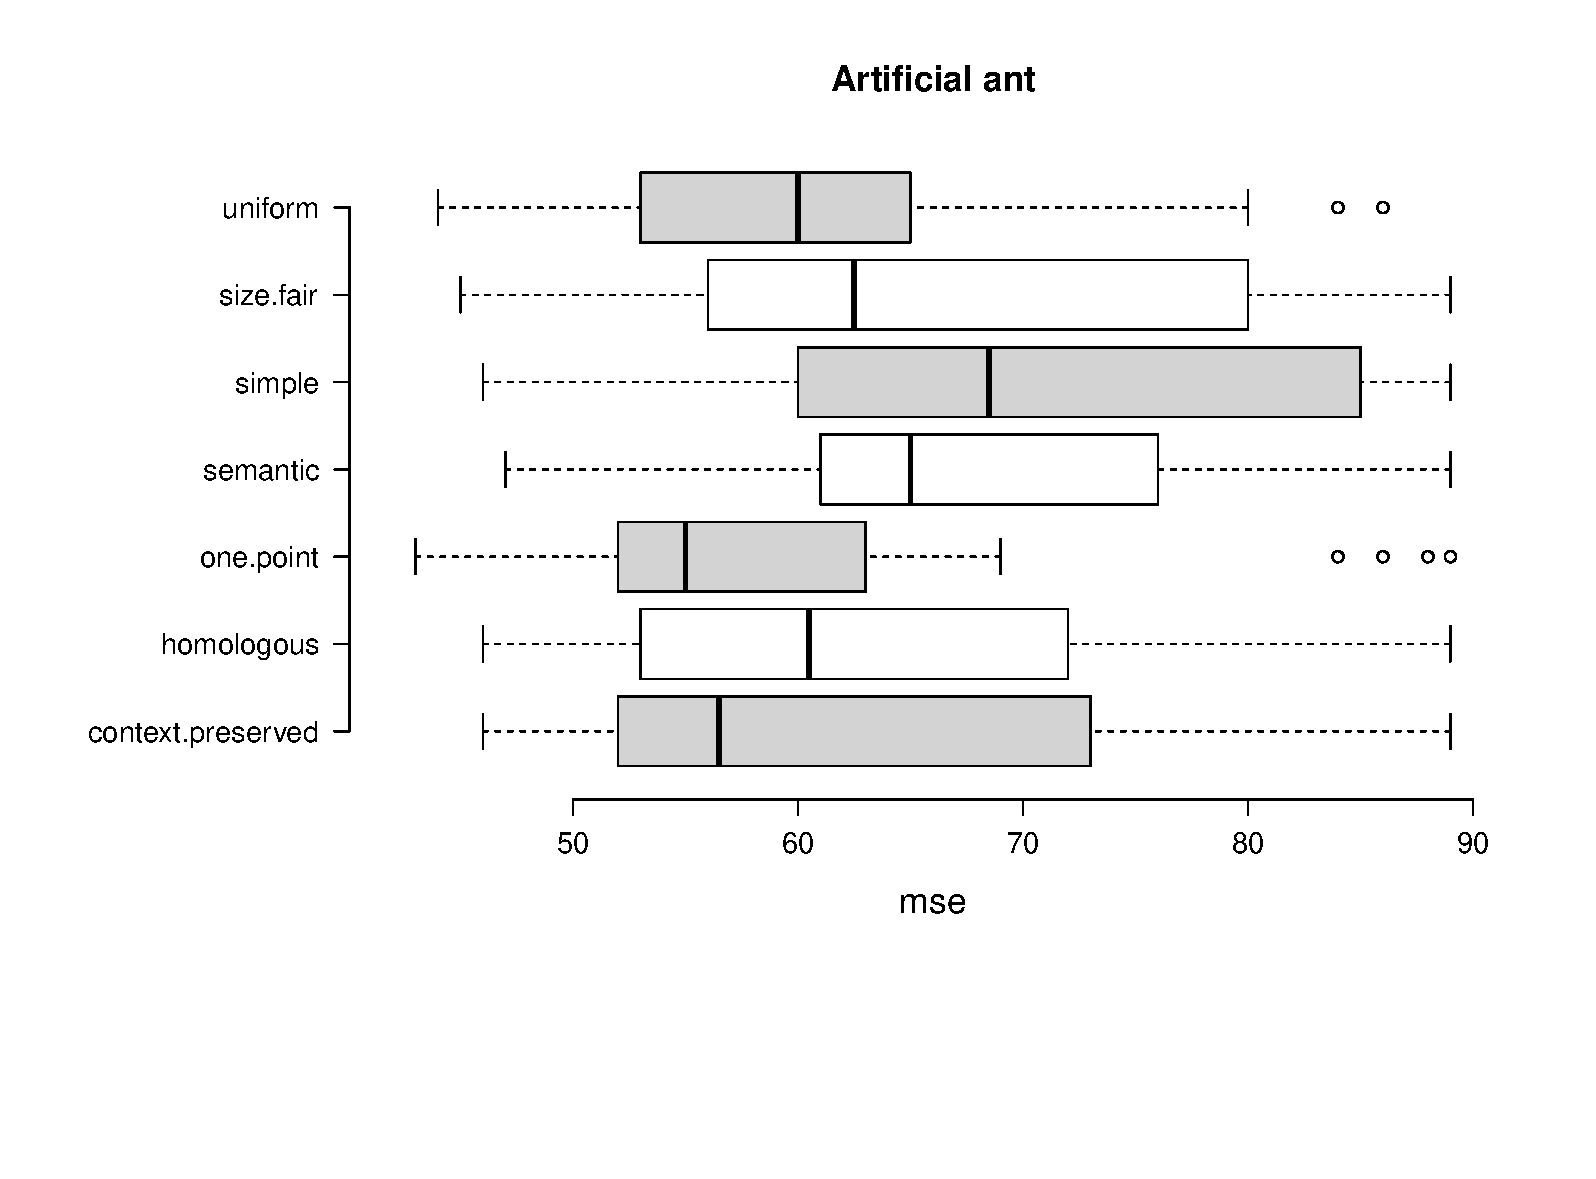
\includegraphics[trim=0cm 4cm 0cm 0cm, scale=0.6]{./slike/boxPlots/ant.eps}
	\caption{Usporedba učinkovitosti pojedinačnih operatora križanja na problem umjetnog mrava}
	\label{antbox}
\end{figure}

Osim ovog eksperimenta, proveden je eksperiment za usporedbu učinkovitosti trenutno najbolje evoluirane jedinke na okolini za učenje, te na dvije, još neviđene okoline za testiranje kroz 100 generacija za svaki operator križanja. Konstanti parametri za ovaj eksperiment jednaki su kao i u prethodnom slučaju. Na slici \ref{trails} prikazana je okolina za učenje i dvije testne okoline.

\begin{figure}[H]
	\centering
	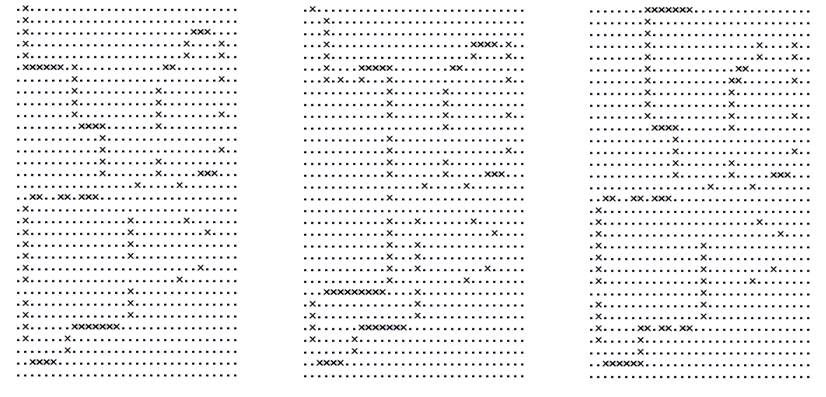
\includegraphics[scale=0.5]{./slike/cross-validation/trails.png}
	\caption{Lijevo: okolina za učenje, sredina: prva testna okolina, desno: druga testna okolina}
	\label{trails}
\end{figure}

Na sljedećim slikama prikazani su rezultati ovih eksperimenata. Na svakoj slici, plavom bojom prikazan je broj pojedene hrane na okolini za učenje, crvenom bojom broj hrane pojedene na prvoj testnoj okolini i zelenom bojom na drugoj testnoj okolini. Ovaj eksperiment proveden je iz razloga što evolucijom jedinke unutar okoline za učenje može doći do njenog prenaučavanja na tu okolinu. Iz tog razloga, kako bi se dobila realnija slika o učinkovitosti operatora, potrebno je usporediti učinkovitost evoluirane jedinke i na nekoj drugoj, jedinci još neviđenoj okolini.

Prikazani rezultati pokazuju kako nijedan operator nije značajno prenaučio najbolju evoluiranu jedinku. Kao što je i očekivano, u okolini za učenje učinkovitost najbolje jedinke u svakom je slučaju nešto veća nego ona u testnim okolinama. To upućuje na laganu prilagodbu jedinke na danu učeču okolinu.
\begin{figure}[H]
	\centering
	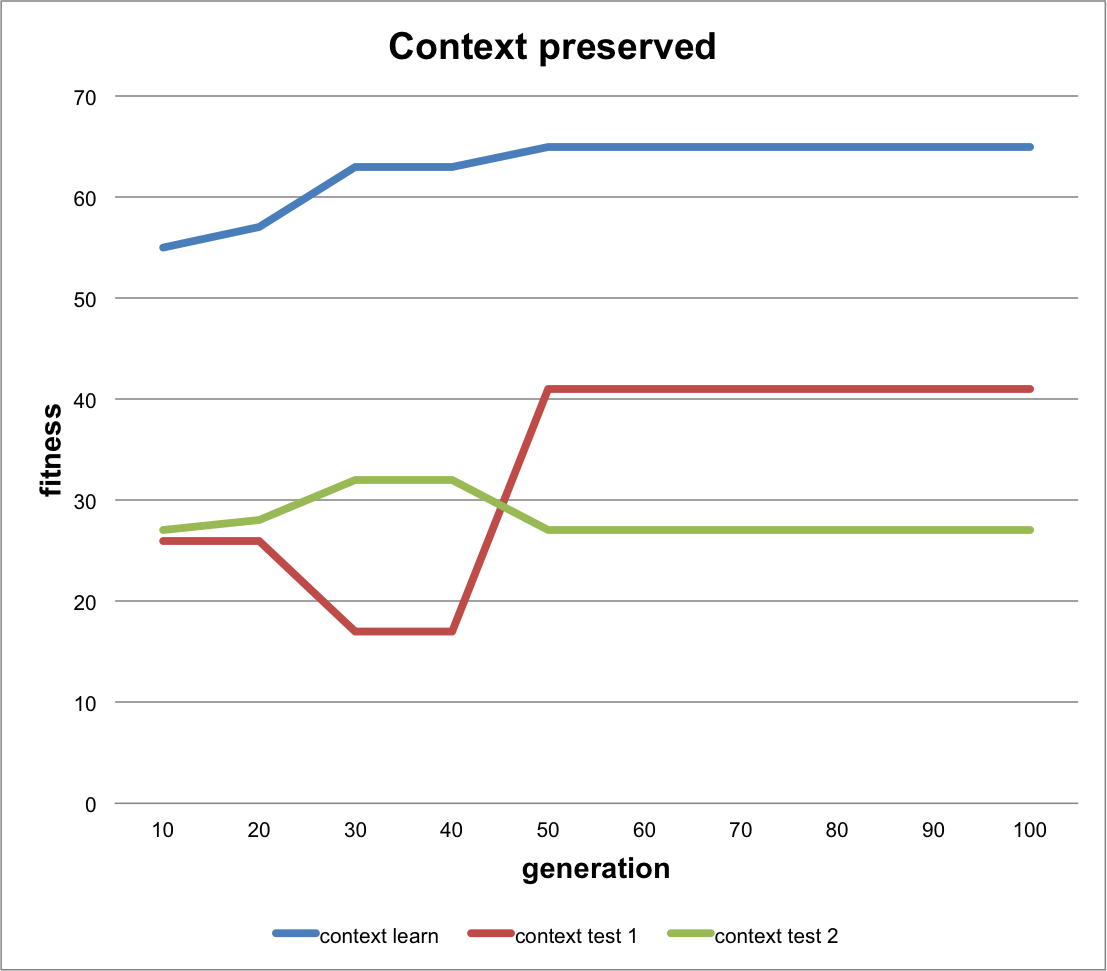
\includegraphics[scale=0.8]{./slike/cross-validation/context.png}
	\caption{Usporedba kvalitete evoluirane jedinke na okolini za učenje i dvije testne okoline za operator križanja s očuvanjem konteksta}
	\label{context}
\end{figure}

\begin{figure}[H]
	\centering
	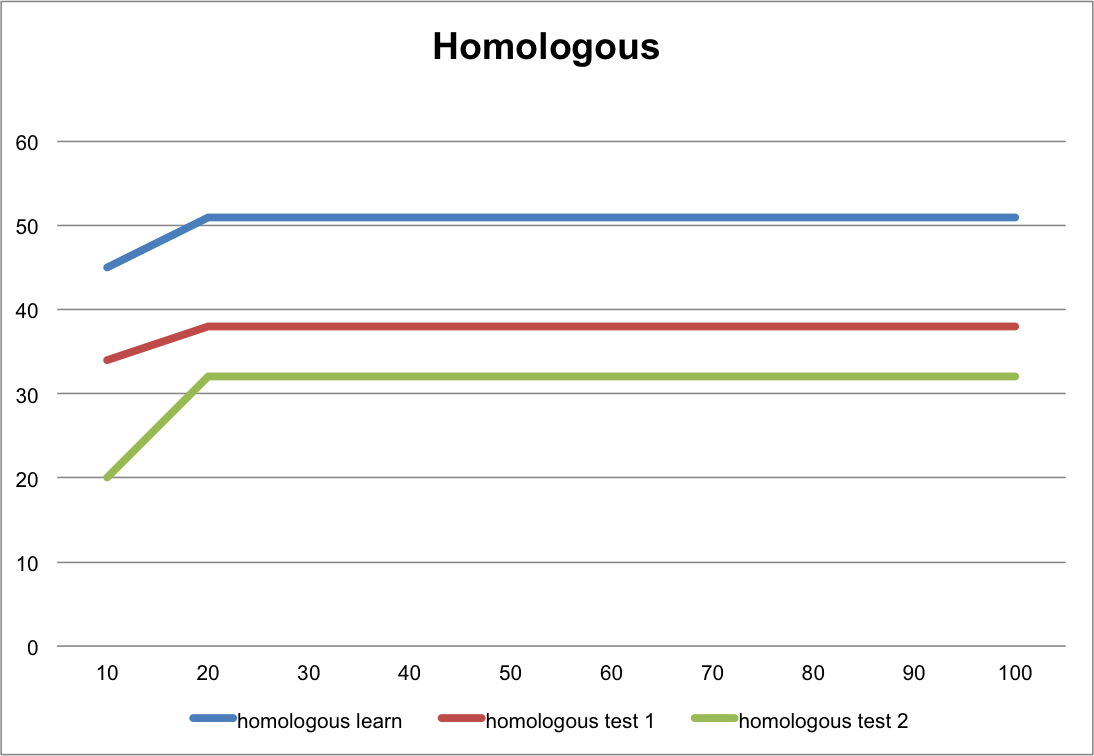
\includegraphics[scale=0.8]{./slike/cross-validation/homo.png}
	\caption{Usporedba kvalitete evoluirane jedinke na okolini za učenje i dvije testne okoline za homologni operator križanja}
	\label{homo}
\end{figure}

\begin{figure}[H]
	\centering
	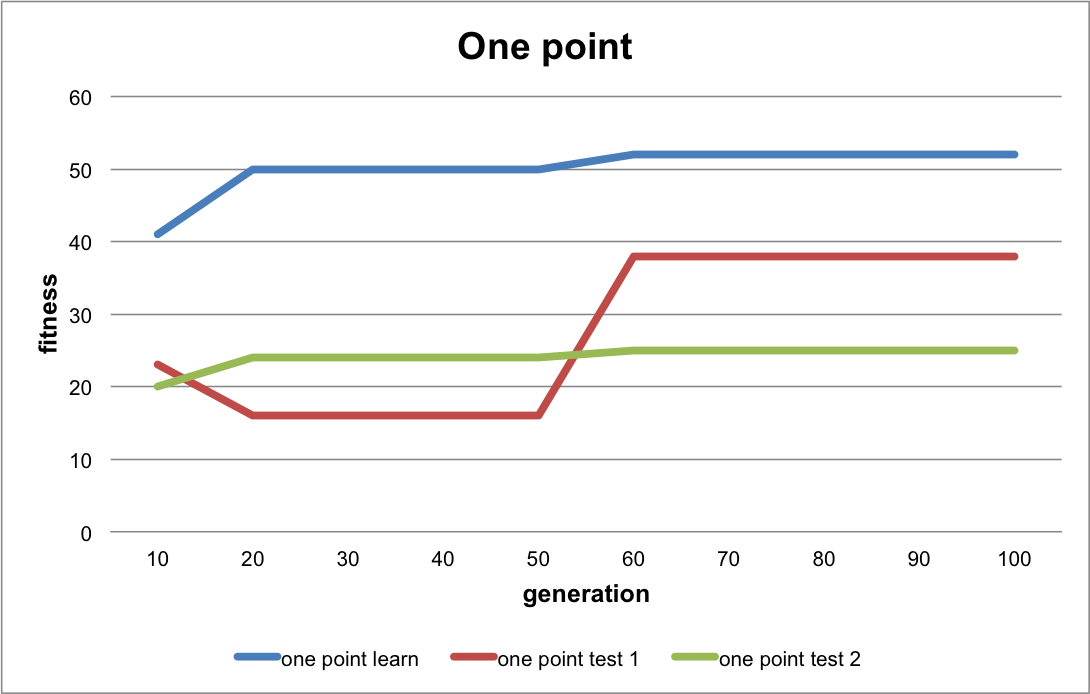
\includegraphics[scale=0.8]{./slike/cross-validation/onepoint.png}
	\caption{Usporedba kvalitete evoluirane jedinke na okolini za učenje i dvije testne okoline za operator križanja s jednom točkom prekida}
	\label{onepoint}
\end{figure}

\begin{figure}[H]
	\centering
	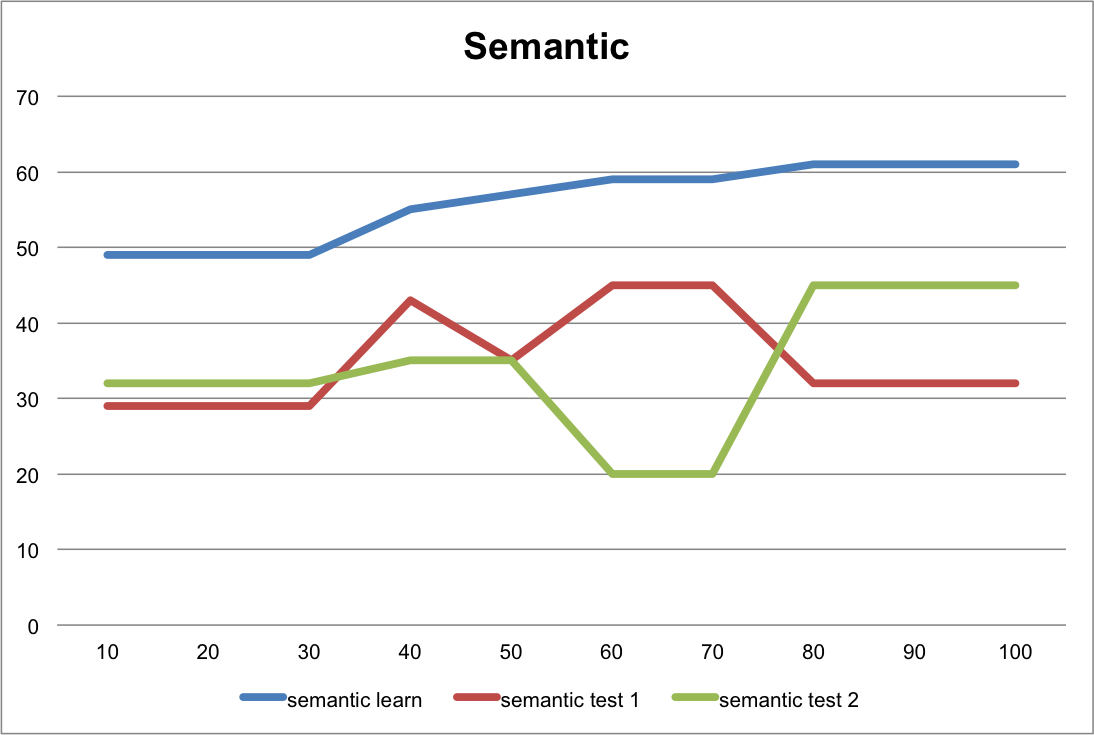
\includegraphics[scale=0.8]{./slike/cross-validation/semantic.png}
	\caption{Usporedba kvalitete evoluirane jedinke na okolini za učenje i dvije testne okoline za kombinaciju semantičkog i jednostavnog križanja u omjeru 1:9}
	\label{semantic}
\end{figure}

\begin{figure}[H]
	\centering
	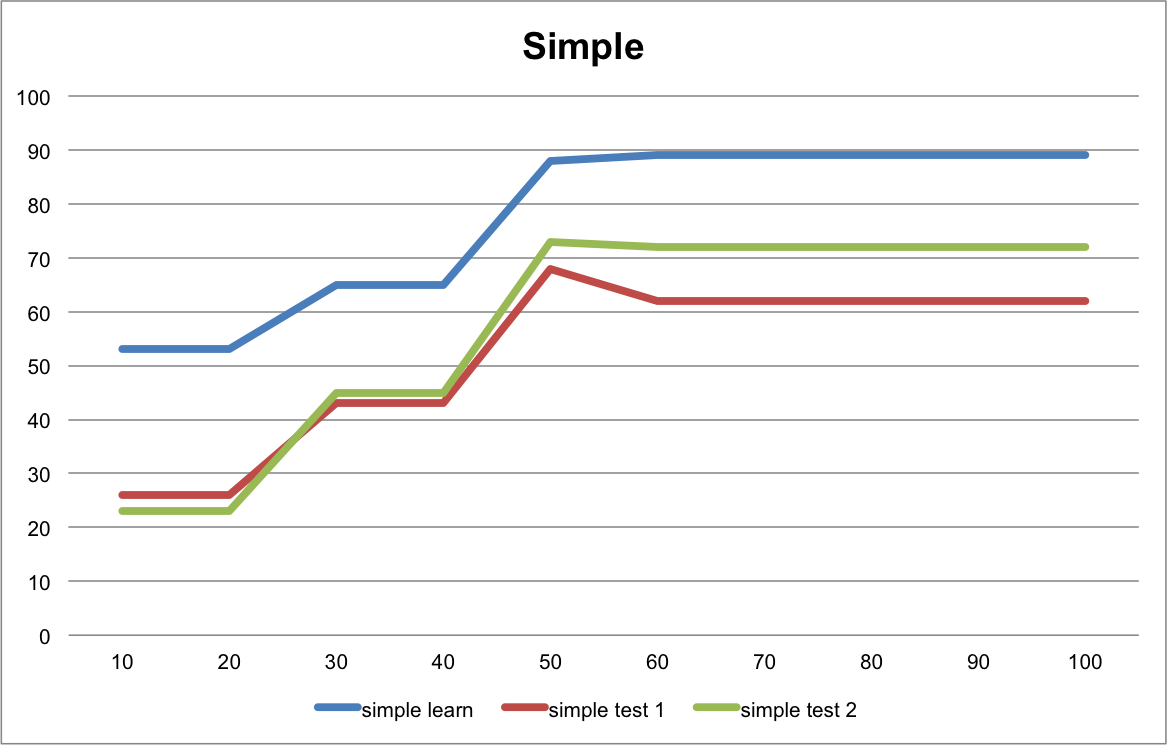
\includegraphics[scale=0.8]{./slike/cross-validation/simple.png}
	\caption{Usporedba kvalitete evoluirane jedinke na okolini za učenje i dvije testne okoline za jednostavni operator križanja}
	\label{simple}
\end{figure}

\begin{figure}[H]
	\centering
	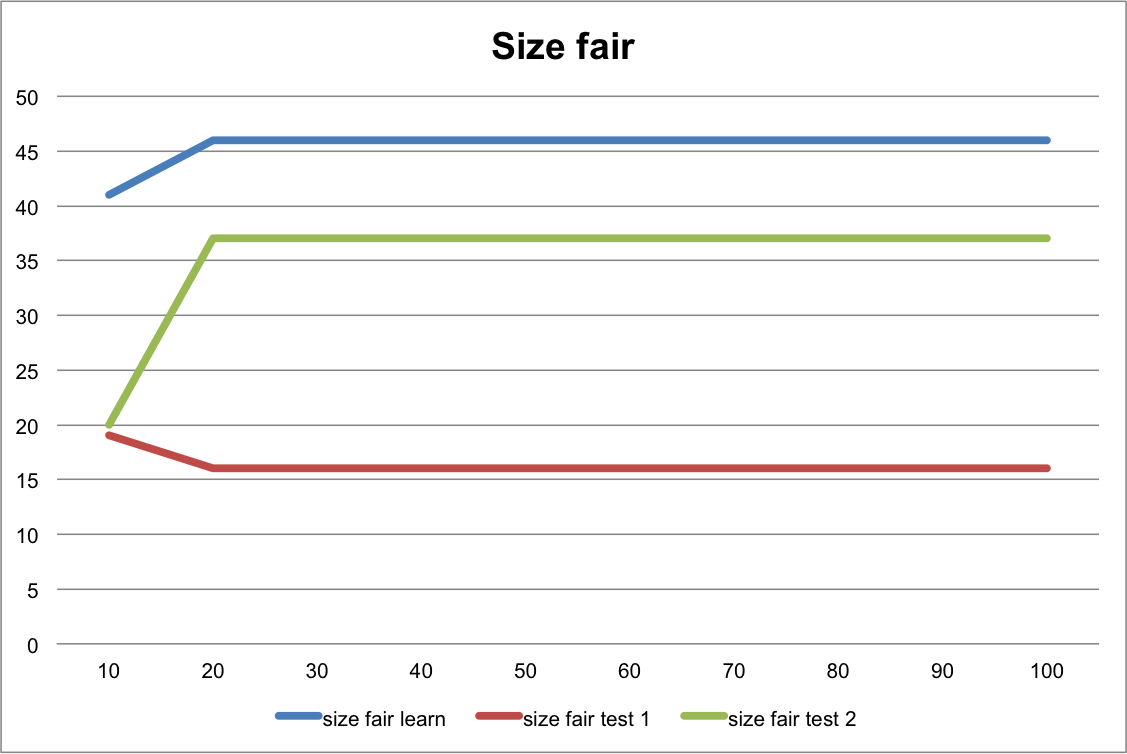
\includegraphics[scale=0.8]{./slike/cross-validation/sizefair.png}
	\caption{Usporedba kvalitete evoluirane jedinke na okolini za učenje i dvije testne okoline za operator križanja koji je pravedan s obzirom na veličinu}
	\label{sizefair}
\end{figure}

\begin{figure}[H]
	\centering
	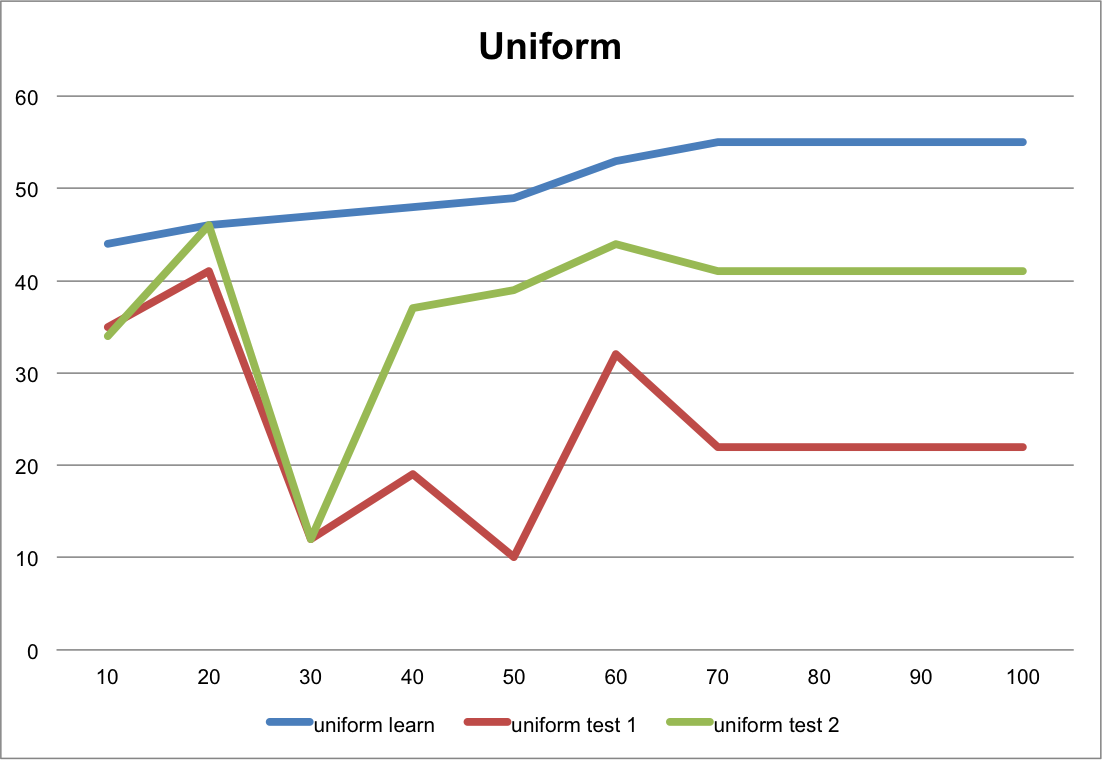
\includegraphics[scale=0.8]{./slike/cross-validation/uniform.png}
	\caption{Usporedba kvalitete evoluirane jedinke na okolini za učenje i dvije testne okoline za uniformni operator križanja}
	\label{uniform}
\end{figure}


\subsubsection{Sveukupni rezultati}
Općenita usporedba svih pojedinačnih operatora križanja prikazana je na tablici \ref{overAllTable}. Tablica za svaki operator prikazuje njegov prosječan rang. Prosječan rang je pritom izračunat kao aritmetička sredina svih rangova koje je taj operator postigao za svaki pojedini problem na kojem je bio testiran.

\begin{table}[H]
 	\centering
 \caption{Prosječan rang učinkovitosti operatora križanja za sve zadane probleme}
 
    \begin{tabular}{| l | l | l |}
    \hline
   \textbf{operator} & \textbf{prosječan rang} & \textbf{ukupan rang} \\ \hline
   simple & 2.0833 & 1\\ \hline
   one point & 5.5 & 8\\ \hline
   context preserved & 4.1667 & 4 \\ \hline
   size fair & 2.25 & 2\\ \hline
   uniform & 4.4167 & 7\\ \hline
   homologous & 4.1667 & 4\\ \hline
   deterministic & 4-2857 & 6\\ \hline
   probabilistic & 7.8571 & 9\\ \hline
   semantic & 2.8333 & 3\\ \hline

 
    \end{tabular}
    
   
    \label{overAllTable}
\end{table}

U većini slučajeva, najučinkovitiji operator ispao je jednostavni operator križanja. Skoro pa jednako učinkovita pokazala se njegova kombinacija sa semantičkim križanjem i križanje pravedno s obzirom na veličinu. Na četvrtom mjestu nalaze se križanje s očuvanjem konteksta i homologno križanje. Zanimljivo je primijetiti kako je križanje s jednom točkom prekida ispalo dosta loše, unatoč njegovoj širokoj upotrebi za rješavanje raznih problema genetskog programiranja. Probabilističko križanje se u gotovo svim eksperimentima pokazalo kao najlošije križanje.

\subsection{Usporedba učinkovitosti kombinacije operatora križanja}

Kako bi se pokazala učinkovitost kombinacija operatora križanja, proveden je eksperiment nad problemom simboličke regresije symb6 (koji se pokazao kao najteži problem koji je rješavan u sklopu ovoga rada). Eksperiment je započeo s uporabom svih operatora križanja od jednom, gdje se svaki pojedini operator koristio s jednakom vjerojatnosti. Nakon toga, oduziman je jedan po jedan operator sve dok se učinkovitost kombinacije mijenjala na bolje. Na grafu \ref{symb6combo} prikazani su rezultati provedenog eksperimenta. Na grafu je izostavljen slučaj u kojem su se upotrijebili svi operatori iz razloga što je prosječna najbolja dobrota u tom slučaju bila znatno veća nego u ostalim slučajevima - kretala se oko broja 250. Prikaz tog rezultata utjecao bi na razlučivost grafa te je iz tog razloga izostavljen. 

\begin{figure}[H]
	\centering
	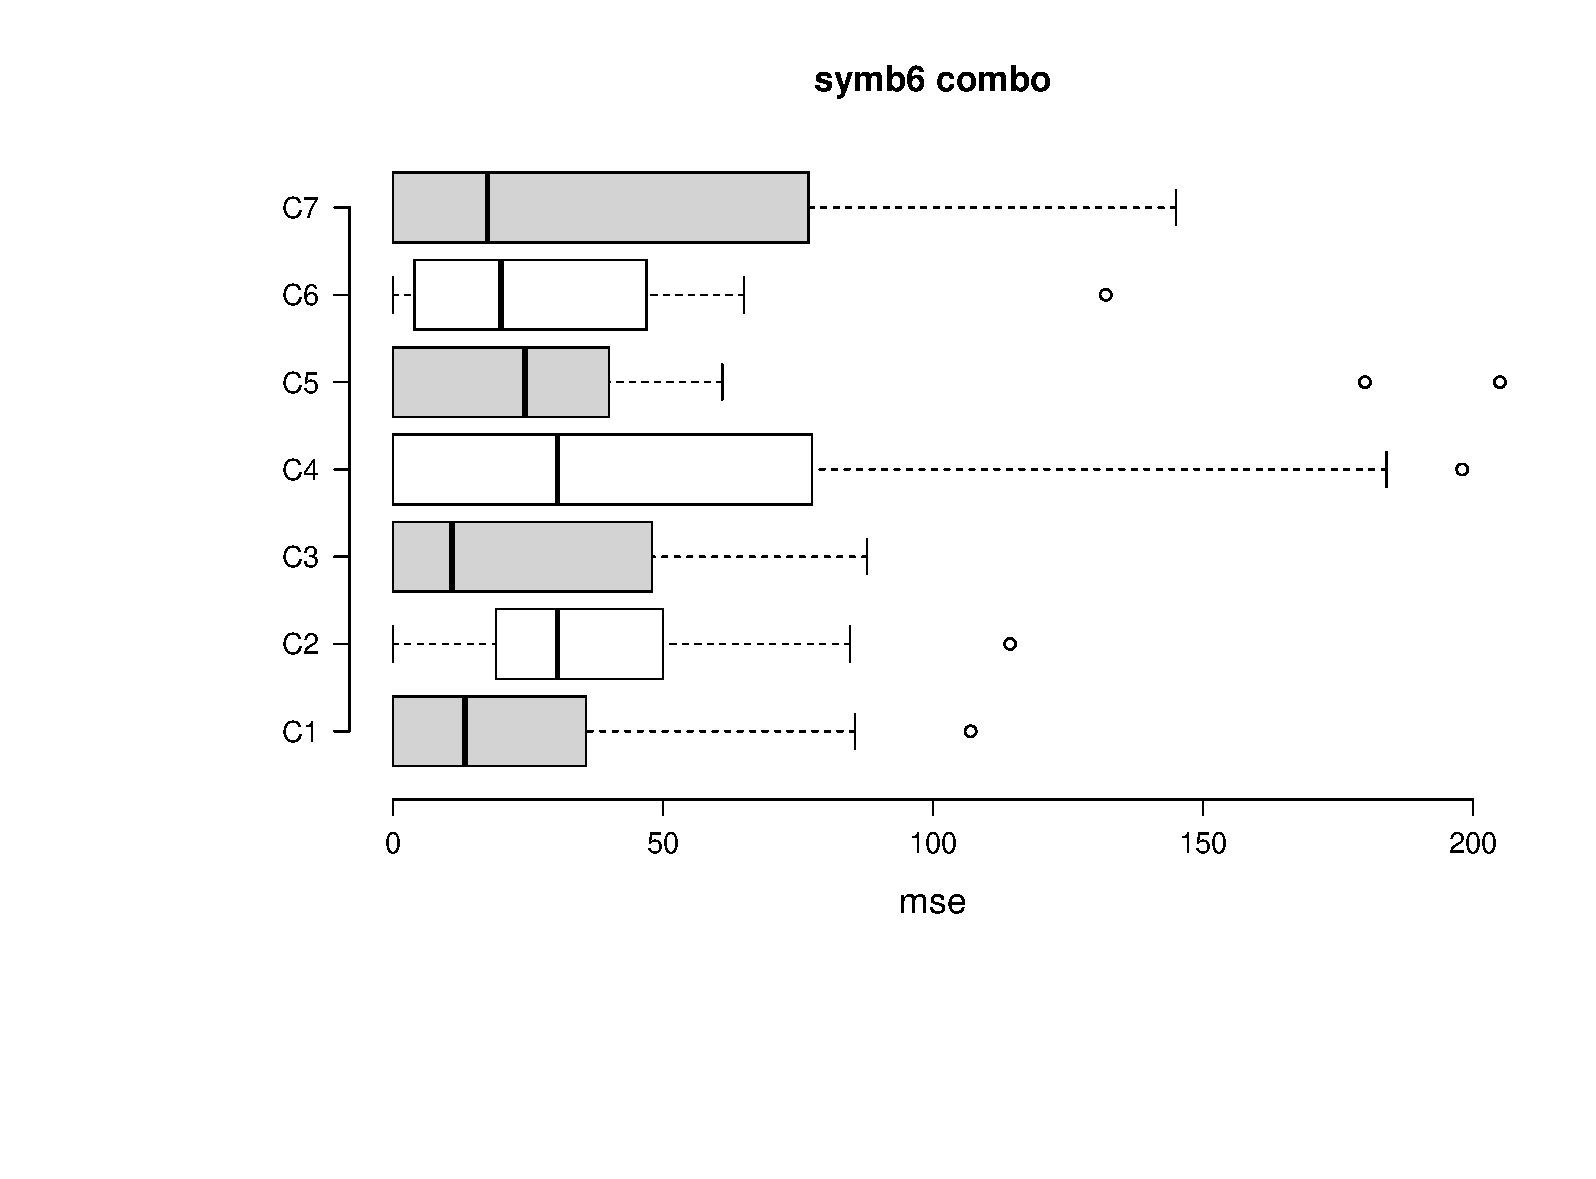
\includegraphics[trim=4cm 4cm 0cm 0cm, scale=0.6]{./slike/boxPlots/symb6-combo.eps}
	\caption{Usporedba učinkovitosti kombinacije operatora križanja na problem simboličke regresije symb6}
	\label{symb6combo}
\end{figure}

Oznake na grafu imaju sljedeća značenja:

\begin{itemize}
\item{C1 - kombinacija svih operatora izuzev probabilističkog}
\item{C2 - kombinacija svih operatora izuzev probabilističkog i križanja s jednom točkom prekida}
\item{C3 - kombinacija svih operatora izuzev probabilističkog i križanja s očuvanjem konteksta}
\item{C4 - kombinacija svih operatora izuzev probabilističkog, križanja s očuvanjem konteksta i homolognog križanja}
\item{C5 - kombinacija svih operatora izuzev probabilističkog, križanja s očuvanjem konteksta i uniformnog križanja}
\item{C6 - kombinacija svih operatora izuzev probabilističkog, križanja s očuvanjem konteksta i determinističkog križanja}
\item{C7 - kombinacija svih operatora izuzev probabilističkog, križanja s očuvanjem konteksta i križanja pravednog s obzirom na veličinu}

\end{itemize}


Iz dobivenih rezultata vidljivo je, kako je najbolja od svih kombinacija ona koja obuhvaća sve operatore osim probabilističkog i križanja s očuvanjem konteksta. Medijan najbolje dobrote ovog operatora iznosi 23.9. Ova vrijednost i dalje je dosta lošija od najbolje dobivene prosječne dobrote s isključivim korištenjem semantičkog i jednostavnog križanja u omjeru 1:9.
\\
\\
Osim ovog, proveden je njemu obrnut eksperiment - krenuvši od jednog, najboljeg operatora, nadodavali su se jedan po jedan od ostalih operatora. No, nakon što je dodan bilo koji operator križanja na početni najbolji (semantički operator), rezultati nisu ispadali bolji od početne vrijednosti. Eksperimentom se nije postiglo ništa relevantno, te iz tog razloga njegovi rezultati nisu prikazani u ovom radu.



\chapter{Zaključak}
Križanje je daleko najvažniji operator evolucijskih algoritama. Bez njega, ne bi bila moguća rekombinacija korisnog genetskog materijala u neki novi, bolji materijal sljedeće generacije. Budući da je danas razvijen poveći broj operatora križanja, pitanje koje se postavlja priikom formulacije problema kojega je potrebno rješiti genetskim programiranjem je sam odabir operatora križanja. 

Ovaj rad pozabavio se upravo tim pitanjem. Usporedivši međusobno operatore križanja za tri najčešće rješavana problema genetskim prigramiranjem - pronalaska logičkih funkcija, simboličke regresije i strojnog učenja, dan je širok pregled učinkovitosti svakog od operatora, kako na pojedini problem, tako i na skup svih problema ispitanih u sklopu ovog rada. 

Zanimljiv zaključak provedenog istraživanja je činjenica da se u većini slučajeva naj-učinkovitijim operatorom pokazao jednostavni operator križanja. Ovaj operator je prvi operator u genetskom programiranju, te je cilj mnogih bio pronaći njegovo poboljšanje. Tako su nastali ostali operatori koji su, kada su predstavljeni, specifičan problem rješavali bolje nego jednostavni operator križanja. Iako su u tim, specifičnim slučajevima donosili određena poboljšanja, ovaj rad pokazao je kako je sigurno dobra polazišna točka u rješavanju nekog problema genetskim programiranjem korištenje jednostavnog križanja.

\chapter{Literatura}
\bibliography{literatura}
\bibliographystyle{unsrt}

\chapter{Sažetak}
\textbf{ \large Ocjena učinkovitosti operatora križanja u genetskom programiranju} \\

U ovom radu dan je pregled i opis postojećih genetskih operatora s naglaskom na operatore križanja. Uz opis svakog pojedinog operatora križanja, prikazani su rezultati do sada izvršenih istraživanja na temu njihove učinkovitosti. Ispitana je učinkovitost algoritma genetskog programiranja s obzirom na odabir operatora križanja za tri najčešće vrste problema koji se rješavaju genetskim programiranjem - simboličku regresiju, pronalazak logičkih funkcija i programe.

\textbf{Ključne riječi}: genetsko programiranje, operatori križanja, evolucija logičkih funkcija, simbolička regresija, evolucija programa, strojno učenje

\chapter{Abstract}
\textbf{ \large Efficiency evaluation of crossover operators in genetic programming } \\

This thesis represents an overview of genetic operators, focusing specifically on the crossover operators. Along with description of every crossover operator, it summarizes results of so far conducted efficiency evaluation experiments. In scope of this thesis, genetic programming effieciency is examined considering the choices of specific crossover operators, solving the three most common problems in genetic programming: symbolic regression, search of logical functions and evolution of programs.

\textbf{Keywords}: genetic programming, crossover operators, evolution of logical functions, symbolic regression, program evolution, machine learning

\end{spacing} 
\end{document}